% Класс документа пока не окончательный, сильно сомневаюсь, что article лучший
\documentclass[a4paper,12pt]{extarticle} 
% Подключаем шрифты,кодировки,русские переносы
\usepackage{cmap}
% подключается пакет, позволяющий улучшить вид пдф документа(как я понял)
\usepackage[utf8x]{inputenc}
% подключаем кодировку шрифтов для вносимых файлов
\usepackage[T2A]{fontenc}
% подключаем кодировку внутреннних шрифтов
\usepackage[russian,english]{babel}
% подключаем перенос и распознование слов, русский в приоритете
\usepackage{indentfirst}
% Отступ в начале абзаца
\usepackage{
	amssymb,
	amsfonts,
	amsmath,
}
% Пакеты американского математ. сообщества, красивый вид формул и текста внутри
\usepackage{
	wrapfig,
	graphicx,
	caption,
	subcaption,
	tikz,
}
% Обтекаемые объекты, рисунки, подписи и прочее
\usepackage{
	pgfplotstable,
	pgfplots,
	booktabs,
	colortbl,
	array
}
\pgfplotsset{compat=newest}
% таблицы, графики
\usepackage{geometry}
\usepackage{fancyhdr}
% границы, контитулы, и прочее


\geometry
	{
	left=2.2cm,
	right=2.2cm,
	bottom=2cm,
	top=2cm,
	}
% границы документа

\usepackage{setspace}
% убирает гигантские размеры оглавления
\linespread{1.3}
% междустрочный интервал

\pagestyle{fancy}
\fancyhead{}
% пустая шапка контитула
\fancyhead[R]{\authors}
% На правой стороне страницы авторы и науч.рук.
\fancyhead[L]{\shortlabname}
 % Слева название лабы
\fancyfoot{}
\fancyfoot[C]{\thepage}
% номер страницы снизу по середине
\renewcommand{\contentsname}{Оглавление}
% переводим на русский язык оглавление
\usepackage{secdot}
\sectiondot{subsection}
% Ставит злосчастные точки в главах, ибо не по госту
% Преамбула почти слизана у Федора Сарафанова https://github.com/FedorSarafanov/RLC/blob/master/text/diss.tex

\usepackage{xcolor}
\usepackage{float}
\usepackage{hyperref}
\hypersetup{unicode=true}
\definecolor{linkcolor}{HTML}{FF7800} % цвет ссылок
\definecolor{urlcolor}{HTML}{133CAC} % цвет гиперссылок
\hypersetup{pdfstartview=FitH,  linkcolor=linkcolor,urlcolor=urlcolor, colorlinks=true}
\begin{document}
	\sloppy
	\def\authors{Есюнин М.В., Есюнин Д.В.}
	% \def\labnum{have no idea}
	\def\labname{Фазовая плоскость лампового генератора}
	\def\shortlabname{Ламповый генератор}
	\def\sciadviser{Половинкин А.В.}
	\renewcommand{\contentsname}{Оглавление}
	\renewcommand{\figurename}{Рис.}
	\renewcommand{\tablename}{Табл.}
	\renewcommand{\vec}{\mathbf}
	\renewcommand{\phi}{\varphi}
	\renewcommand{\kappa}{\varkappa}
	% нормальный вид вектора, фи и каппа
	\renewcommand{\Re}{\operatorname{Re}}
	\renewcommand{\Im}{\operatorname{Im}}
	% меняем номрмальное начертание Re and Im
	\begin{titlepage}

\begin{center}

	\textsc{Нижегородский государственный университет имени Н.\,И. Лобачевского}
	\vskip 4pt \hrule \vskip 8pt
	\textsc{Радиофизический факультет}

	\vfill

	{\Large\labname}

\end{center}

\vfill

\begin{flushright}
	{Работу выполнили студенты\\ \authors\\ 430 группы\\ \vskip 14pt научный руководитель:\\ \sciadviser}
\end{flushright}

\vfill

\begin{center}
	Нижний Новгород, \the\year
\end{center}

\end{titlepage}
	\begin{spacing}{1.2}
		\tableofcontents
	\end{spacing}
\subsubsection*{Цель работы} Изучение различных режимов возбуждения лампового генератора и установление зависимости амплитуды и частоты автоколебаний от параметров системы.

Аппаратом теоретического рассмотрения является метод Ван-дер-Поля. Полученные с его помощью результаты сравниваются с результатами экспериментального исследования фазовой плоскости изучаемой системы. 

\section{Теоретическая часть}
 
\subsection{ Метод Ван-дер-Поля}
Слабонелинейные квазиконсервативные системы могут совершать периодические движения с постоянной амплитудой, определяемой свойствами системы. Таким периодическим движениям на фазовой плоскости соответствуют изолированные замкнутые фазовые траектории, называемые {\itshapeпредельными циклами}.

Предельный цикл будет устойчивым, если все фазовые траектории, начинающиеся в малой окрестности предельного цикла, будут асимптотически приближаться при $t\to\infty$.

Динамические системы, а фазовом портрете которых имеется, по крайней мере, один устойчивый предельный цикл, называются автоколебательными. 

Будем считать, что система описывается уравнением вида 
\begin{equation}
\label{eq:1}
\ddot{x}+x=\mu f(x,\dot{x}),
\end{equation}
где  $f(x,\dot{x})$ - нелинейная ограниченная функция 

~$\mu$ - малый безразмерный параметр.

Нас интересуют периодические решения. Метод Ван-дер-Поля позволяет задачу отыскания периодических решений уравнения \eqref{eq:1} свести к несравненно более простой - задаче нахождения состояний равновесия так называемых укороченных уравнений. Перейдем к их составлению.

При $\mu=0$ уравнение \eqref{eq:1} описывает обычный гармонический осциллятор, и его решение можно записать в виде:

$$x=A\cos(t+\varphi)=A\cos\theta,$$
\begin{equation}
\label{eq:2}
\dot{x}=y=-A\sin(t+\varphi)=-A\sin\theta,
\end{equation}
где А и $\varphi$ - произвольные постоянные, имеющие физический смысл амплитуды и фазы колебаний. 

Решение можно представить и в комплексной форме в виде: 
\begin{gather}
\label{eq:3}
x=ze^{jt}+z^*e^{-jt},\\\notag
\dot{x}=y=j(ze^{jt}-z^*e^{-jt}),
\end{gather}
где z и $z^*$ - произвольные постоянные, являющиеся комплексной и комплексно сопряженной амплитудами.  

Решение вида  \eqref{eq:3} легко сводится к виду \eqref{eq:2}, если положить $$z=\rho e^{j\varphi}, z^*=\rho e^{-j\varphi}$$

В результате получим:

\begin{center}
$x=\rho(e^{j(t+\varphi)}+e^{-j(t+\varphi)})=2\rho \cos(t+\varphi)$,

$\dot{x}=y=j\rho(e^{j(t+\varphi)}-e^{-j(t+\varphi)})=2\rho \sin(t+\varphi)$.
\end{center}
Следовательно, 
\begin{gather}
\label{eq:4}
|z|=|z^*|=\rho=\frac{A}{2},\\\notag
argz=-argz^*=\varphi.
\end{gather}

При $\mu \ne 0$, но сколь угодно малом, решение уравнения \eqref{eq:1}  не должно существенно отличаться от решения для линейного осциллятора, поэтому будем его искать в виде \eqref{eq:2} , считая теперь А и $\varphi$ не постоянными величинами, а некоторыми неизвестными функциями времени:

\begin{center}
$\dot{x}=\dot{A} \cos\theta-A(1+\dot \varphi)\sin\theta=-A\sin\theta$, $\theta=t+\varphi$
\end{center}

Откуда следует $$\dot{A}\cos\theta-A\dot \varphi \sin\theta=0.$$

Подставляя решение  \eqref{eq:2} в уравнение  \eqref{eq:1}, будем иметь $$\dot{A}\sin\theta+a\dot \varphi \cos\theta=-\mu f(A\cos\theta;-A\sin\theta).$$
Разрешая два последних уравнения относительно $\dot{A}$ и $\dot{\varphi}$, получаем систему
\begin{gather}
\label{eq:5}
\dot{A}=-\mu f(A\cos\theta;-A\sin\theta)\sin\theta,\\\notag
A\dot{\varphi}=-\mu f(A\cos\theta;-A\sin\theta) \cos\theta.
\end{gather}
адекватную уравнению \eqref{eq:1}, но записанную в других переменных, называемых переменными Ван-дер-Поля. Полученная система не является более простой по сравнению с уравнением \eqref{eq:1}. Однако, если учесть, что $\mu \ll 1$, то из нее можно получить приближенную, значительно более простую систему.

Правая часть системы  \eqref{eq:5} является периодической функцией явно входящего времени $\theta=t+\varphi$ и зависит от А и $\varphi$. Поскольку  А и $\varphi$ являются медленно меняющимися функциями времени, то можно их считать постоянными на периоде быстрых осцилляций. Воспользуемся этим и, проинтегрировав уравнения, определим средние значения за период $T=2\pi$. Заметим, что интегрирование можно проводить не по времени, а по $\theta=t+\varphi$. В результате получим систему
\begin{gather}
\label{eq:6}
\frac{dA}{dt}=-\frac{\mu}{2\pi}\int\limits_\theta^{\theta+2\pi} f(A\cos\theta;-A\sin\theta)\sin\theta d\theta,\\\notag
\frac{d\varphi}{dt}=-\frac{\mu}{2\pi A}\int\limits_\theta^{\theta+2\pi} f(A\cos\theta;-A\sin\theta)\cos\theta d\theta.
\end{gather}

Запишем ее в виде
   
\begin{equation}
\label{eq:7}
\frac{dA}{dt}=\mu \Phi(A),~\frac{d\varphi}{dt}=\mu \phi(A),
\end{equation}
где $\Phi(A)$ и $\phi(A)$ - средние за период значения периодических функций, зависящие только от А: $$-f(A\cos\theta;-A\sin\theta)\sin\theta,~~f(-\frac{1}{A} \cos\theta;-A\sin\theta)\cos\theta.$$

Полученные уравнения  \eqref{eq:7} и называются системой укороченных или усредненных уравнений. Эта система определяет амплитуду и фазу квазигармонических колебаний исходной системы, описываемой уравнением  \eqref{eq:1}. Если мы найдем решения укороченных уравнений, то с помощью соотношений  \eqref{eq:2} получим приближенные решения исходной системы.

Нас интересует частный пример, когда $\phi(A)=0$

Этот случай довольно часто встречается на практике, например, при рассмотрении режимов работы ламповых генераторов без учета сеточных токов. Тогда система укороченных уравнений  \eqref{eq:7} принимает вид:
\begin{equation}
\label{eq:8}
\frac{dA}{dt}=\mu \Phi(A),~ \varphi=\varphi_0 = Const
\end{equation}

Первое уравнение может исследоваться независимо от второго, т.к. оно зависит только от А. Координаты состояния равновесия $A_{0}$ на фазовой прямой А есть корни уравнения $\Phi(A_{0})=0$

При этом характеристическое уравнение имеет вид $p-\mu \Phi^{'}_{A}(A_{0}) = 0$ и состояние равновесия будет устойчивым, если $$\frac{d\Phi}{dA}= \Phi^{'}_{A}(A_{0}) <0$$
и неустойчивым при выполнении обратного неравенства.


\begin{figure}[h!]
	\centering
    \begin{minipage}{0.49\linewidth}
        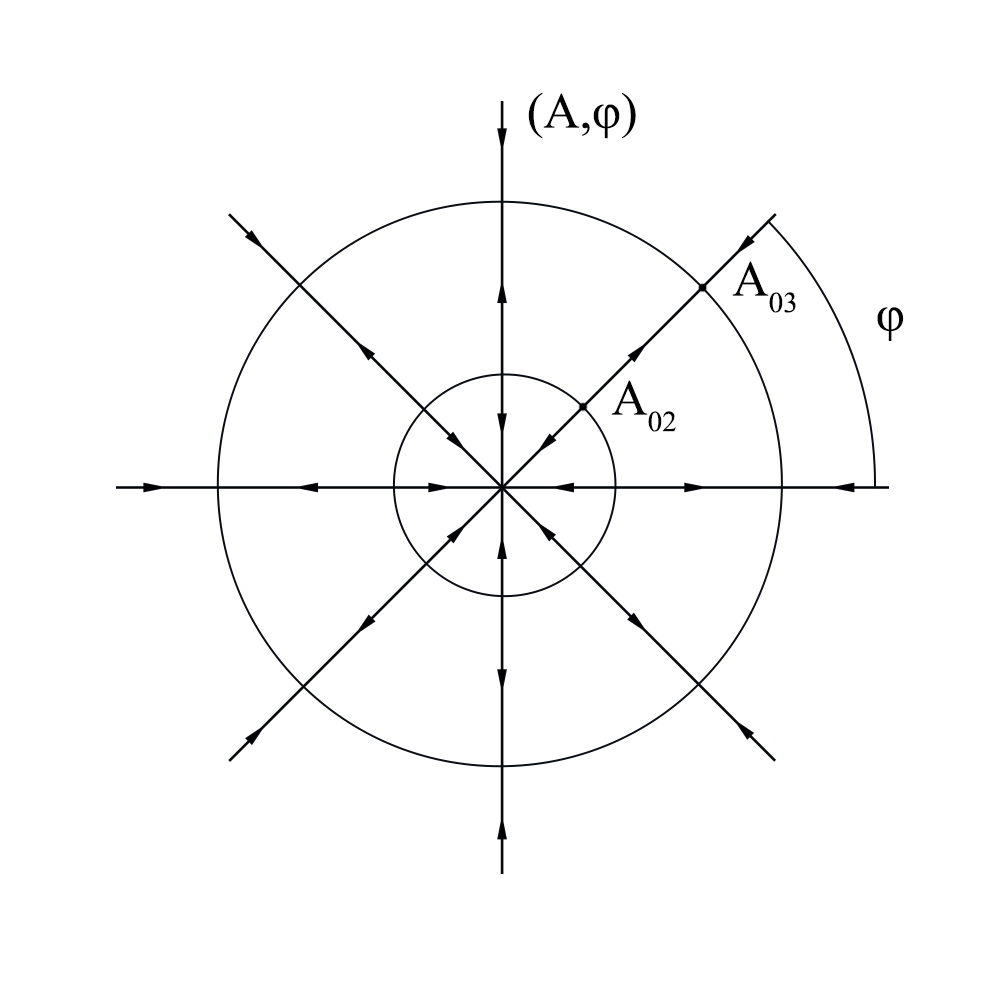
\includegraphics[width=\linewidth]{photo/pics/Ris1.png} 
        \caption{} 
        \label{fig:1}
    \end{minipage}
\hfill     
    \begin{minipage}{0.49\linewidth}
        \centering
        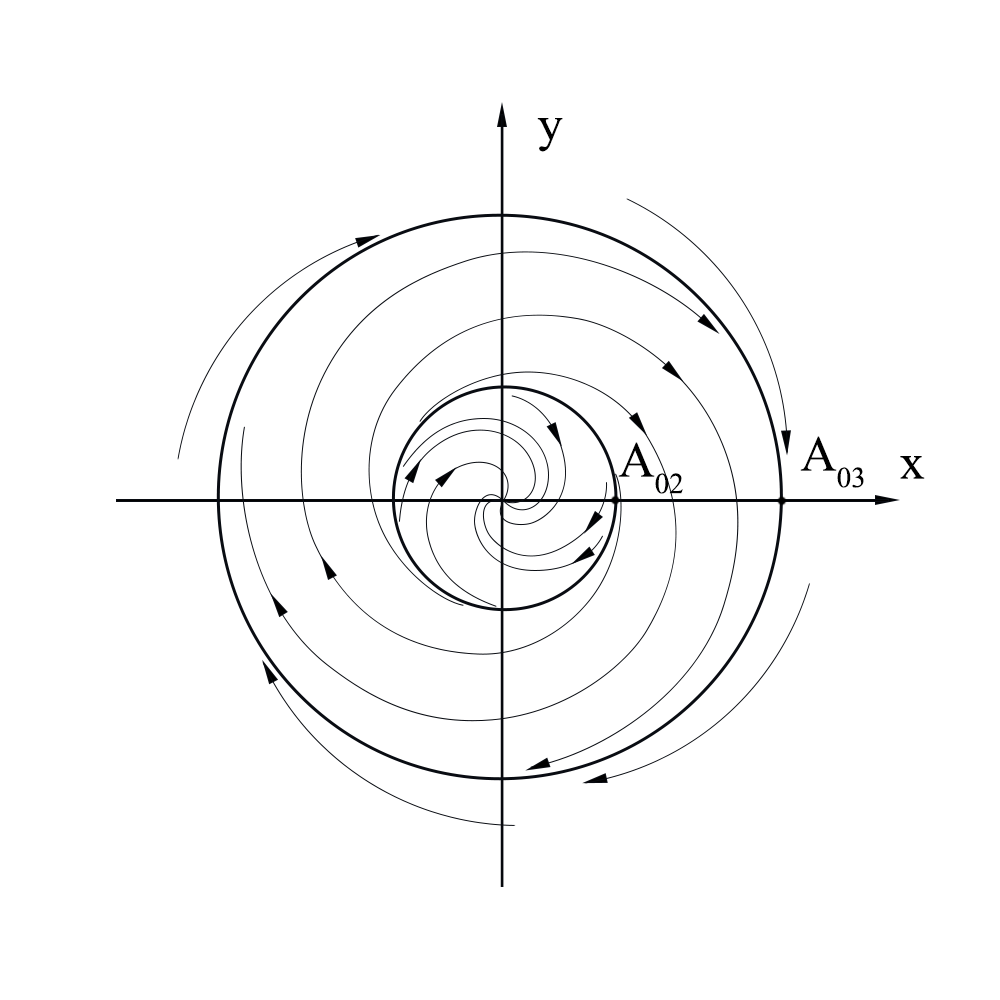
\includegraphics[width=\linewidth]{photo/pics/Ris2.png}
        \caption{} 
        \label{fig:2}
    \end{minipage}
\end{figure} 

Картина фазовых траекторий на плоскости переменных Ван-дер-Поля для системы с тремя состояниями равновесия \eqref{eq:8} (где A и $\phi$ полярные координаты), выглядит следующим образом (рис.\ref{fig:1}): 

Переход к переменным xy осуществляется с помощью формул преобразования  \eqref{eq:2}. Фазовый портрет на плоскости ху может быть получен, если вращать плоскость Ван-дер-Поля по часовой стрелке с круговой частотой $\omega=1$ вокруг начала координат. Тогда окружности, состоящие из состояний равновесия, перейдут в круговой предельные циклы, имеющие те же радиусы $A_{0i}$. Предельные циклы будут устойчивы, если устойчивы состояния равновесия укороченных уравнений, и наоборот. Остальные траектории, представляющие собой отрезки прямых на плоскости переменных Ван-дер-Поля, преобразуются на плоскости ху в спирали (рис.2).

\subsection{Исходные и укороченные уравнения}

В работе исследуется LC-генератор с контуром в цепи сетки рис.\ref{fig:3}, относящийся к разряду квазисинусоидальных автоколебательных систем.

\begin{figure}[h!]
	\centering
    \begin{minipage}{0.49\linewidth}
        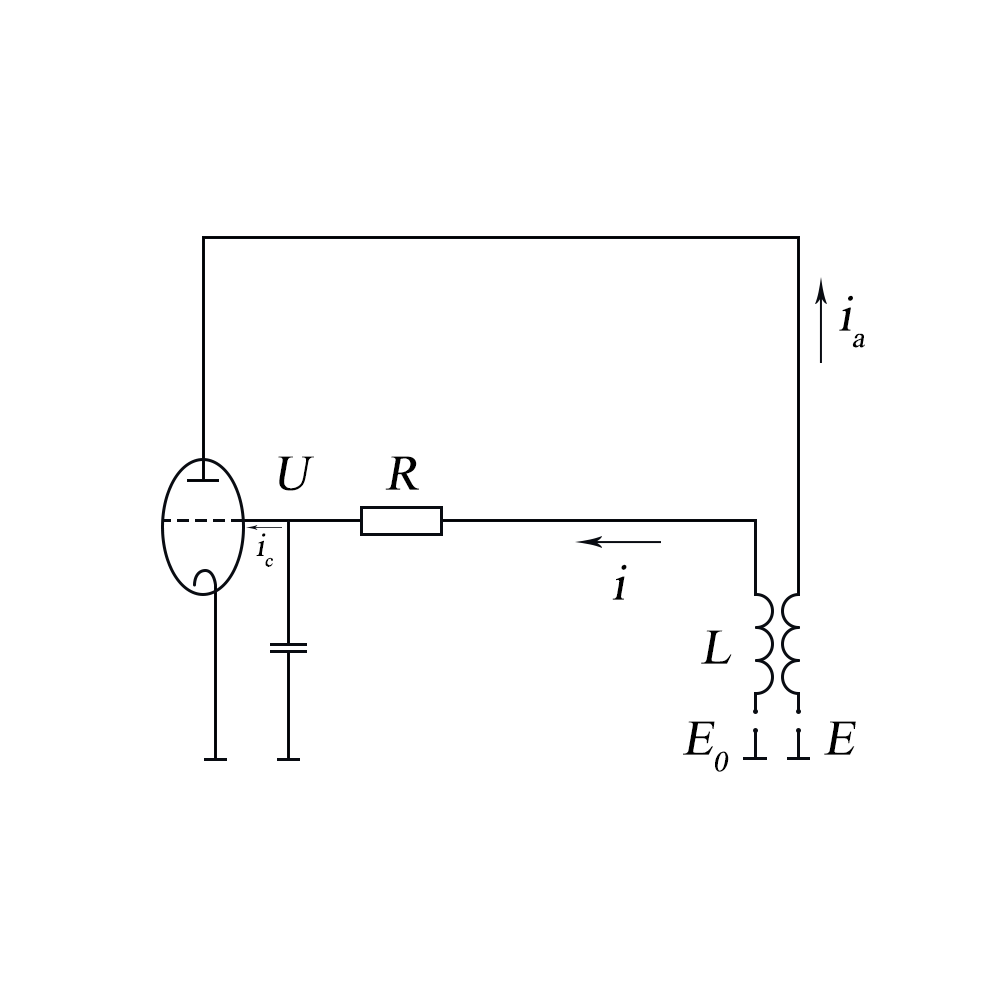
\includegraphics[width=\linewidth]{photo/pics/Ris3.png}
        \vspace{-60pt}
        \caption{}
        \label{fig:3}
    \end{minipage}
\hfill     
    \begin{minipage}{0.49\linewidth}
        \centering
        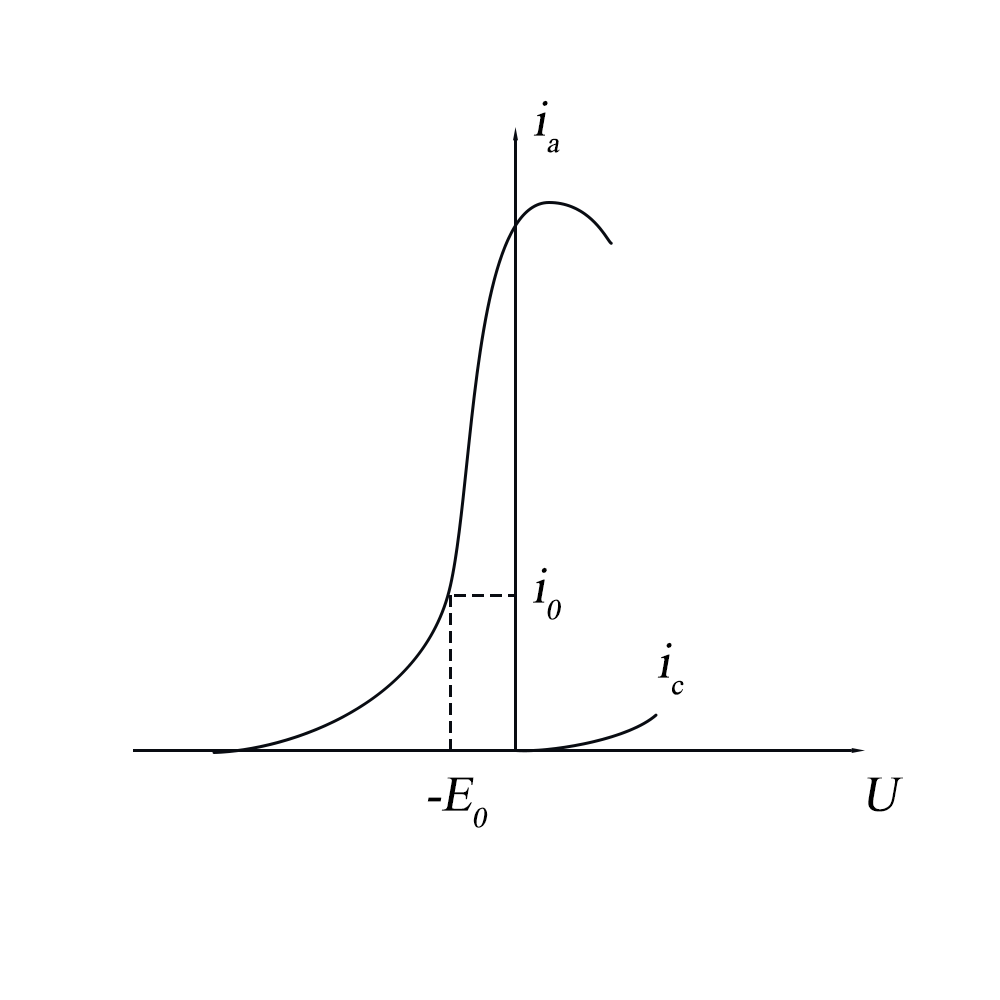
\includegraphics[width=\linewidth]{photo/pics/Ris4.png}
        \vspace{-60pt}
        \caption{} 
        \label{fig:4}
    \end{minipage} 
\end{figure}   

Отправной точкой теоретического исследования этой системы являются уравнения Кирхгофа, которые, с учетом обозначений, принятых на рис.\ref{fig:3}, запишутся в виде:
\begin{gather}
\label{eq:9}
L\frac{di}{dt}+Ri+U=M\frac{di_a}{dt}-E_0,\\\notag
i=C\frac{dU}{dt}+i_c,
\end{gather}
где $i_a$ и $i_c$ - анодные и сеточные токи лампы, зависящие в общем случае от анодного и сеточного напряжений. В дальнейшем будем учитывать их зависимость только от сеточных напряжений, то есть пренебрежем реакцией анода. Качественный вид анодно-сеточной и сеточной характеристик приведен на рис.\ref{fig:4}. В проводимом рассмотрении эти нелинейные функции будут аппроксимированы полиномами. 

Исключив из системы \eqref{eq:9} ток и введя новые переменные
\begin{equation}
\label{eq:10}
x=U+E_0, ~ \tau=\frac{t}{\sqrt{LC}},
\end{equation}
запишем исходную систему  \eqref{eq:9} в виде одного уравнения второго порядка
\begin{equation}
\label{eq:11}
\ddot{x}+x=\frac{d}{d\tau}[-\delta x+\sigma f_1(x)]-f_2(x)
\end{equation}

Здесь $\sigma=\frac{M}{\sqrt{LC}}>0$, $\alpha=\frac{L}{M}$, $\delta=R\sqrt{\frac{C}{L}}$, $f_1=(i_a-\alpha i_c)$, $f_2=Ri_c$. Заметим, что функция $f_1(x)$ включает в себя разность анодного и сеточного токов, но т.к. сеточный ток меньше анодного, то не будет большой ошибкой считать $f_1=i_a$.

Укороченные уравнения для данной системы будут иметь вид:
\begin{gather}
\label{eq:12}
\dot\rho=-\frac{1}{2} (\delta-\sigma \bar{f_1}(\rho^2))\rho,\\\notag
\dot\varphi=\frac{1}{2}\bar{f_2}(\rho^2).
\end{gather}

Здесь $\bar{f_1}(\rho^2)$  определяется анодно-сеточной характеристикой лампы и влияет на условия возбуждения генератора и амплитуду установившихся колебаний;  $\bar{f_2}(\rho^2)$ определяется сеточной характеристикой и влияет на поправку к частоте. Для отыскания установившихся (стационарных) значений амплитуды автоколебаний достаточно найти устойчивые состояния равновесия  $\bar{\rho}$  первого из уравнений системы \eqref{eq:12}. При этом из второго уравнения системы найдем поправку к частоте автоколебаний:
\begin{equation}
\label{eq:13}
\Delta \omega=\frac{\bar{f_2}(\bar{\rho}^2)}{2}
\end{equation}

задающую величину, на которую частота колебаний генератора будет отличатся от частоты колебаний контура. Тем самым, в режиме установившихся автоколебаний будем иметь:

\begin{equation}
\label{eq:14}
\varphi=\frac{\bar{f_2}(\bar{\rho}^2)}{2}\tau+\varphi_0
\end{equation}

\begin{equation}
\label{eq:15}
x=2\bar{\rho}\cos(\tau+\varphi)=2\bar{\rho}\cos[(1+\frac{\bar{f_2}(\bar{\rho})}{2})\tau+\varphi_0].
\end{equation}

\subsection{Стационарные режимы работы генератора}

Прежде чем переходить к изучению различных режимов работы лампового генератора, выясним, при каких условиях справедлива та или иная аппроксимация нелинейной характеристики лампы. На динамику генератора и стационарные режимы его работы влияют только нечетные члены степенного ряда нелинейной характеристики $f_{1}(x)$. Выделим из нелинейной функции нечетную ее часть с помощью соотношения
\begin{equation}
\label{eq:16}
f_H(x)=\frac{f(x)-f(-x)}{2}
\end{equation}

Вид нечетной части характеристики, а, следовательно, и возможная её аппроксимация зависят от выбора рабочей точки, положение которой определяется постоянным смещением $E_{0}$ на сетке лампы. Рассмотрим возможные аппроксимации нелинейной функции $f_{1}$ и, как следствие, различные режимы работы генератора.

{\bfseries 1.} Напряжение смещения $E_{0}$ на управляющей сетке лампы (рабочая точка) выбрано так, что нечетная часть анодно-сеточной характеристики имеет вид,  приведенный на рис.5. Это возможно в том случае, когда напряжение смещения задано в точке максимальной крутизны характеристики. При этом функцию $f_{1}$ достаточно точно можно представить в виде полинома третьей степени, причем аппроксимация будет справедлива для части кривой, обозначенной сплошной линией на рис.\ref{fig:5}:
\begin{wrapfigure}{r}{.4\textwidth}
    \begin{center}
        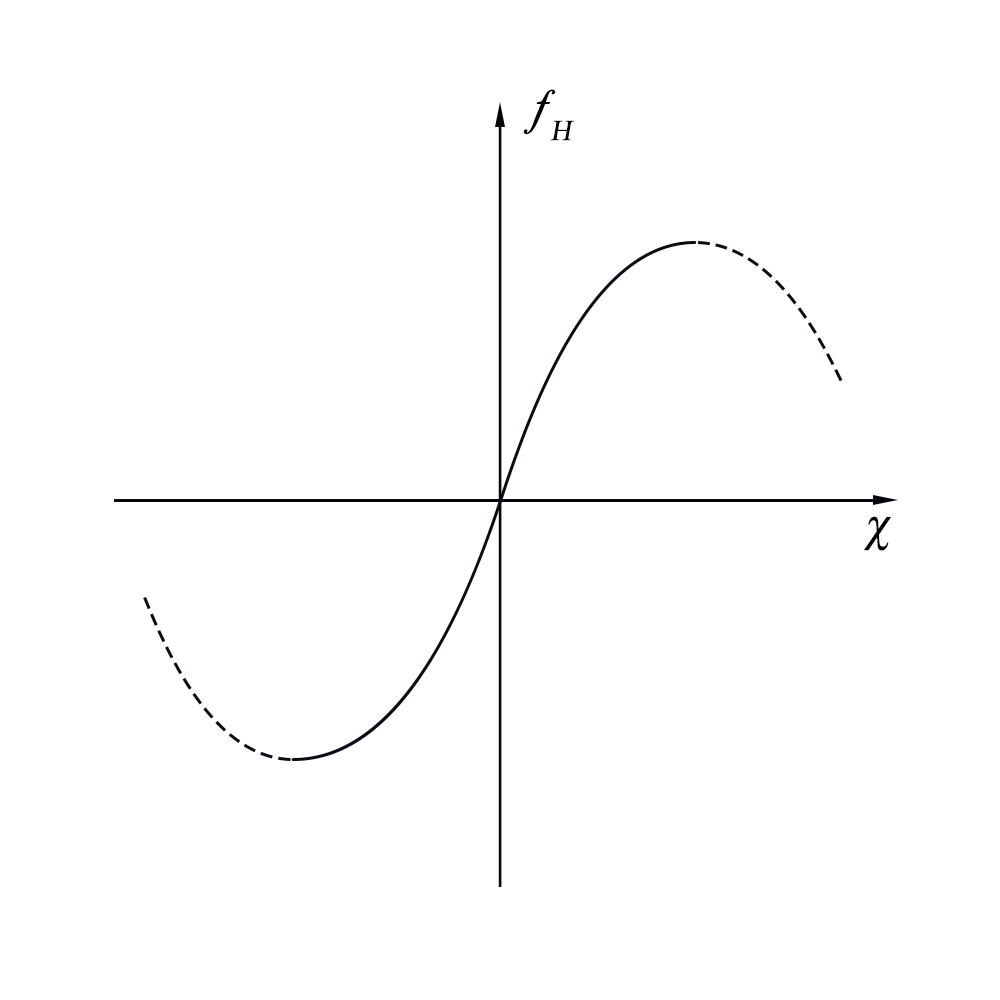
\includegraphics[width=\linewidth]{photo/pics/Ris5.png}
        \vspace{-40pt}
        \caption{}
        \label{fig:5}
    \end{center}
\end{wrapfigure}   
\begin{equation}
\label{eq:17}
f_1(x)=a_1+\frac{a_2}{2}x^2-\frac{a_3}{6}x^3
\end{equation}

Здесь и в дальнейшем все коэффициенты аппроксимирующего полинома будем считать положительным. Для аппроксимации \eqref{eq:17} средняя крутизна анодно-сеточной характеристики, т.е. функция $\bar{f}_1$ примет вид:
\begin{equation}
\label{eq:18}
\bar{f}_1(\rho^2)=a_1-\frac{a_3}{2}\rho^2.
\end{equation}

В этом случае закон изменения амплитуды колебаний, согласно системе \eqref{eq:12}  будет определяться следующим уравнением: 

\begin{equation}
\label{eq:19}
\dot\rho=-\rho \bar{F}(\rho),
\end{equation}

\noindent где $\bar{F}(\rho)=\frac{[\delta-\sigma(a_1-\frac{a_3}{2}\rho^2)]}{2}$. Приравнивая правую часть этого уравнения нулю, получим стационарные значения амплитуд колебаний:
\begin{equation}
\label{eq:20}
\bar{\rho}_1=0,~ \bar{\rho}_2=\sqrt\frac{2(-\delta+\sigma a_1)}{\sigma a_3}.
\end{equation}

Их устойчивость определяется корнями следующего характеристического уравнения:

\begin{equation}
\label{eq:21}
\rho=\frac{d}{d\rho}[-\rho\bar{F}(\rho)]\bigg|_{\rho=\bar{\rho}}=-\bar{F}(\bar{\rho})-\bar{\rho}\bar{F}^{'}(\bar{\rho})
\end{equation}

Состояние системы с нулевым значением $\bar{\rho}$ (невозбужденный генератор) будет устойчивым при $\bar{F}(0)>0$, т.е. при $\sigma=\frac{\delta}{a_1}$ и неустойчивым в противном случае. Второе стационарное состояние устойчиво, если $\bar{F}^{'}(\bar{\rho})=\sigma a_3 \bar{\rho_2}>0$, что выполняется при выбранных знаках коэффициентов. Выражение \eqref{eq:21} определяет зависимость амплитуды колебаний от линейного декремента $\delta=\frac{R\sqrt{C}}{\sqrt{L}}$, коэффициента связи $\sigma=\frac{M}{\sqrt{LC}}>0$, и коэффициентов аппроксимации анодно-сеточной характеристики $a_1$ и $a_3$. Можно построить бифуркационные диаграммы, выражающие зависимость $\bar{\rho}_2$ от любого из перечисленных параметров. Зависимость $\bar{\rho}_2$ от параметра $\sigma$ (величина обратной связи) приведена на рис.6, где точками обозначены устойчивые состояния, а крестиками - неустойчивые. из приведенной диаграммы видно, что схема возбуждается при условии $\sigma>\frac{\delta}{a_1}$, или, если перейти к параметрам схемы, при $M>\frac{RC}{a_1}$. В этом неравенстве величина $a_1$ - крутизна анодно-сеточной характеристики в рабочей точке. Точка $\sigma=\frac{\delta}{a_1}$ на бифуркационной диаграмме называется {\itshapeточкой бифуркации} - здесь качественно меняется поведение системы.
\begin{center}
    \begin{minipage}{0.3\linewidth}
            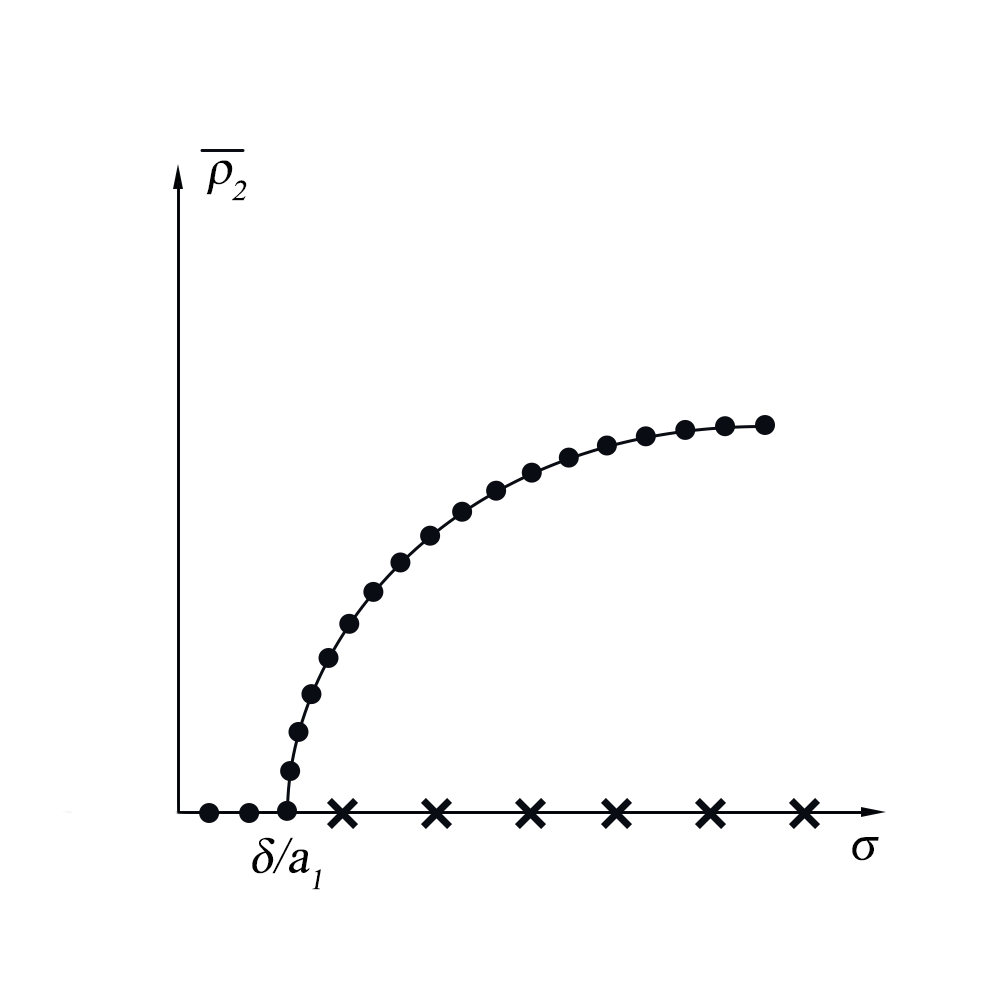
\includegraphics[width=\linewidth]{photo/pics/Ris6.png}
            \captionof{figure}{}
            \label{fig:6}
    \end{minipage}
    \begin{minipage}[t]{0.6\linewidth}
            \begin{minipage}{0.45\linewidth}
                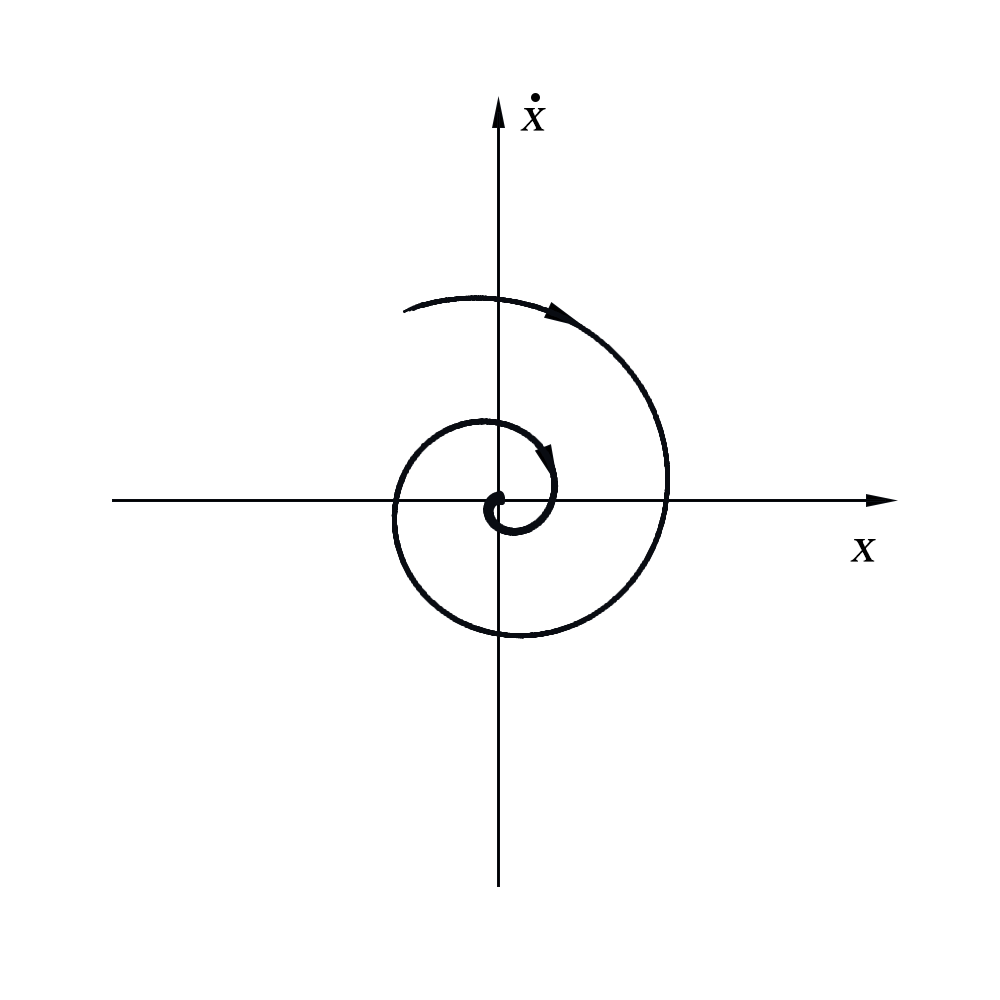
\includegraphics[width=\linewidth]{photo/pics/Ris7a.png}
                \captionof{subfigure}{}
                \label{fig:7}
            \end{minipage}
            \begin{minipage}{0.45\linewidth}
                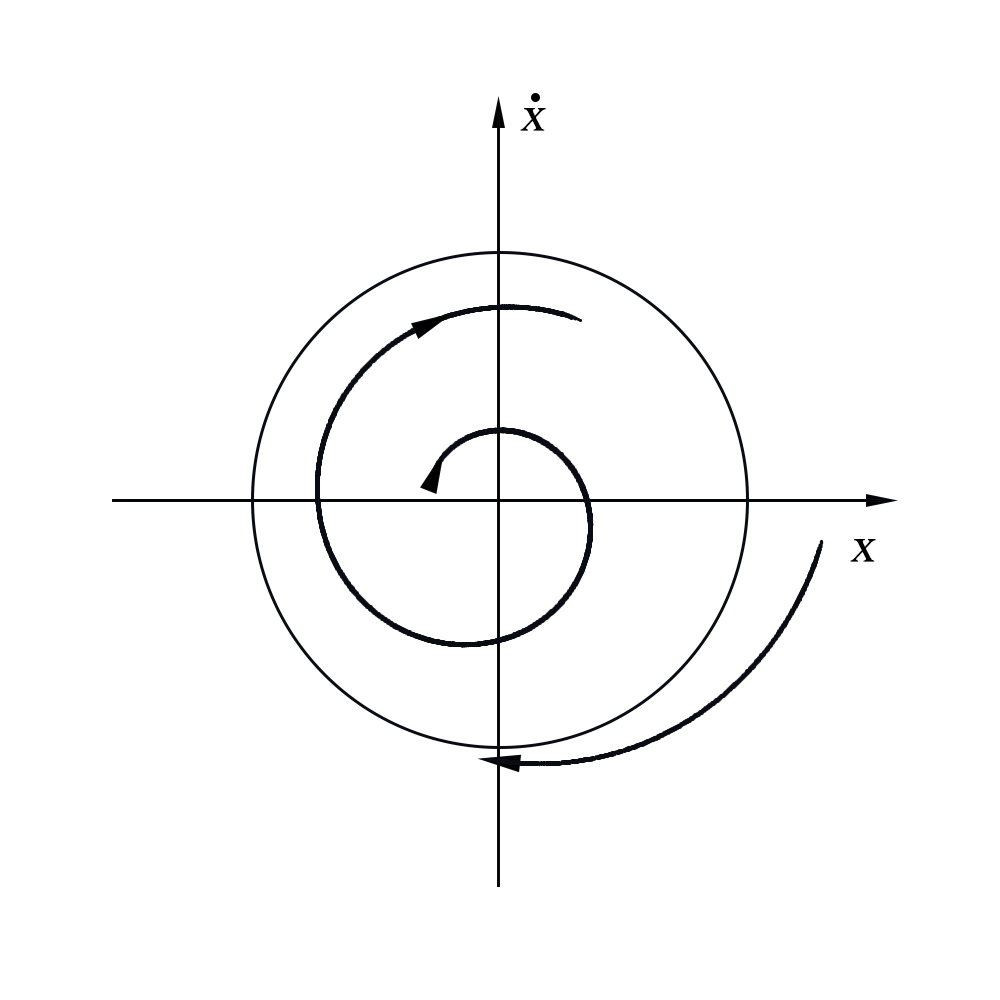
\includegraphics[width=\linewidth]{photo/pics/Ris7b.png} 
                \captionof{subfigure}{} 
                \label{fig:8}
            \end{minipage}
    \end{minipage}
\end{center}
  
Фазовые портреты системы при $\sigma<\frac{\delta}{a_1}$ и $\sigma>\frac{\delta}{a_1}$ приведены на рис.\ref{fig:7} и рис.\ref{fig:8}. Как видно из рис.\ref{fig:6} и рис.\ref{fig:8}, предельный цикл устанавливается при сколь угодно малых начальных условиях, то есть генератор обладает {\itshapeмягким режимом} возбуждения по 
отношению к начальным условиям. Термин "мягкий" может употребляться в другом смысле - в качестве характеристики типа генератора, отличающегося плавным нарастанием установившегося значения амплитуды колебаний при медленном и непрерывном изменении параметра обратной связи. Приведенная на рис.\ref{fig:6} 
бифуркационная диаграмма соответствует именно такому типу генератора.  

{\bfseries 2.}Рабочая точка выбрана так, что нечетная часть характеристики имеет вид, приведенный на рис.\ref{fig:8a}. Этому случаю чаще всего отвечают напряжения смещения, близкие к напряжению осечки лампы. При этом характеристику лампы необходимо аппроксимировать полиномом не ниже пятой степени. Такой аппроксимации соответствует средняя крутизна
% \afterpage{\clearpage} 
\begin{equation}
\label{eq:22}
\bar{f}_1(\rho^2)=a_1+\frac{a_3}{2}\rho^2-\frac{a_5}{12}\rho^4.
\end{equation}
и, следовательно, уравнение, определяющее стационарные значения амплитуды автоколебаний принимает вид
\begin{equation}
\label{eq:23}
\rho[\delta-\sigma(a_1+\frac{a_3}{2}\rho^2-\frac{a_5}{12}\rho^4)]=0.
\end{equation}

\begin{figure}[h!]
    \vspace{-20pt}
    \centering
    \begin{minipage}{0.49\linewidth}
    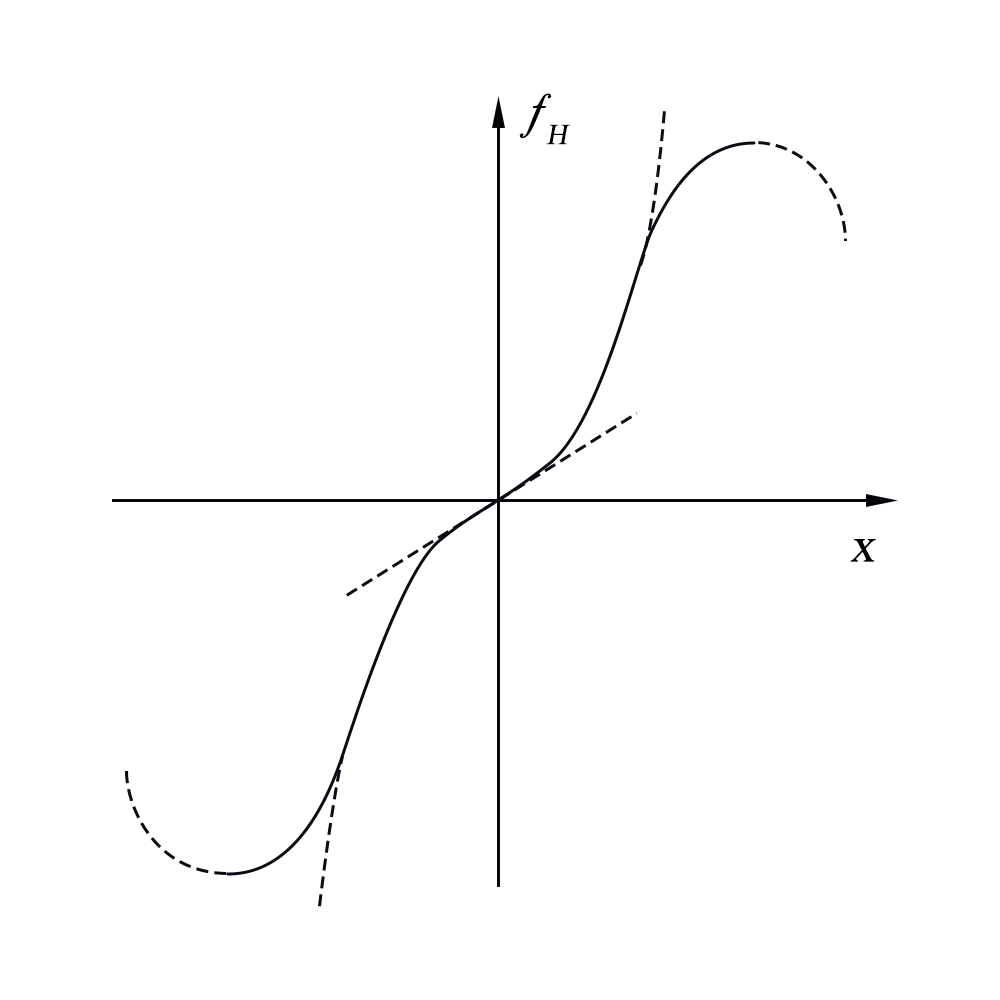
\includegraphics[width=\linewidth]{photo/pics/Ris8.png}
    \caption{}
    \label{fig:8a}
    \end{minipage}
    \begin{minipage}{0.49\linewidth}
    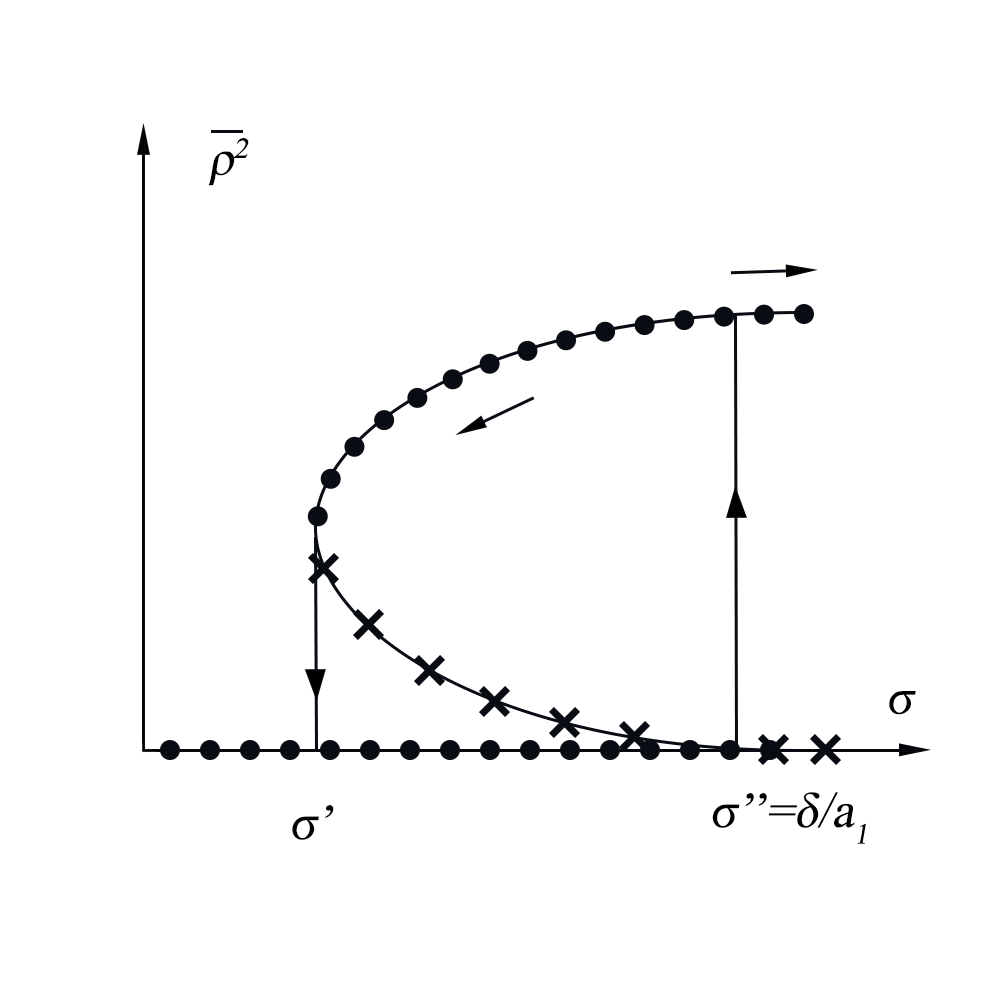
\includegraphics[width=\linewidth]{photo/pics/Ris9.png}
    \caption{}
    \label{fig:9}
    \end{minipage}
\end{figure}
% \begin{wrapfigure}{l}[0.4\linewidth]
% 	\centering
%     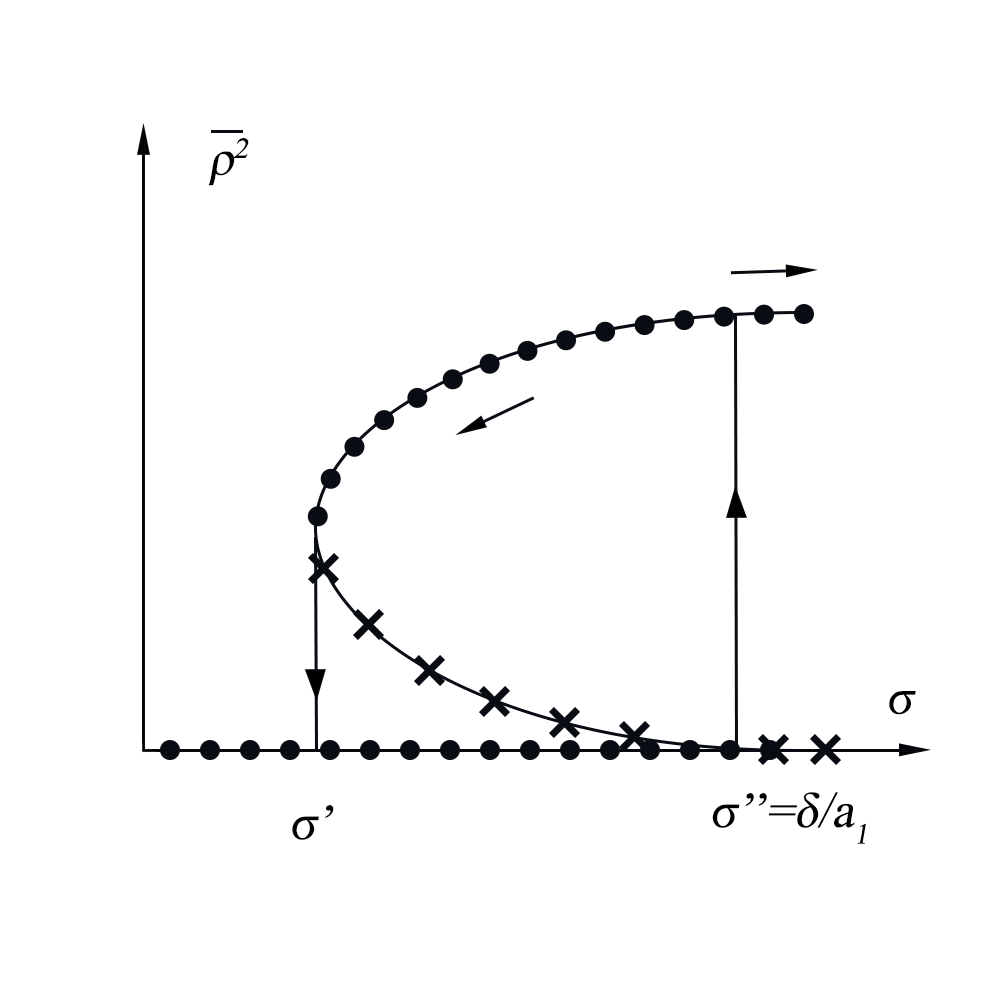
\includegraphics[width=0.4\linewidth]{photo/pics/Ris9.png}
%     \vspace{-30pt}
%     \caption{}
%     \label{fig:9}
% \end{wrapfigure} 
Бифуркационная диаграмма для этого случая приведена на рис.\ref{fig:9}. Из него следует, что при значениях параметра $\sigma$, лежащих в интервале ${\sigma}'\textless \sigma \textless {\sigma}"$, возникновение автоколебаний возможно лишь, если начальное значение $\rho$ превышает соответствующее пороговое значение. В этом случае говорят о {\itshapeжестком режиме} возбуждения генератора. Бифуркационная диаграмма, изображенная на рис.9 характеризуется гистерезисным эффектом установления срыва автоколебаний при непрерывном изменении параметра $\sigma$. Системы с таким видом бифуркационной диаграммы относят к жёсткому типу генераторов. 
Для них, согласно рис.9, мягкое возбуждение возможно лишь при $\sigma>\sigma^"$, т.е. за пределами области гистерезиса. На рис.10 a,b и c приведены фазовые портреты такого генератора для различных значений параметра $\sigma$.

\begin{center}
\vspace{-20pt}
    \begin{figure}[h!]
        \begin{minipage}{0.32\linewidth}
            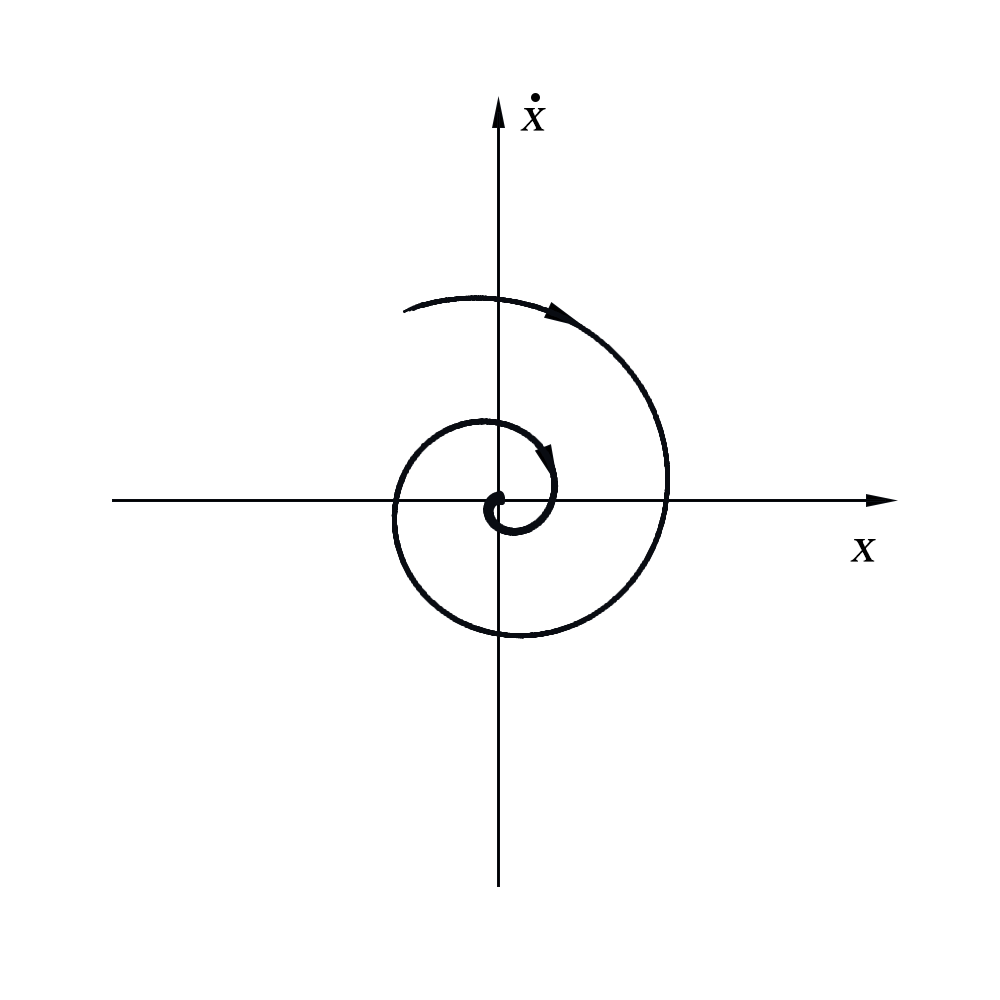
\includegraphics[width=\linewidth]{photo/pics/Ris10a.png}
            \vspace{-30pt}
            \captionof{subfigure}{} 
            \label{fig:10}
        \end{minipage}
    \begin{minipage}{0.32\linewidth}
        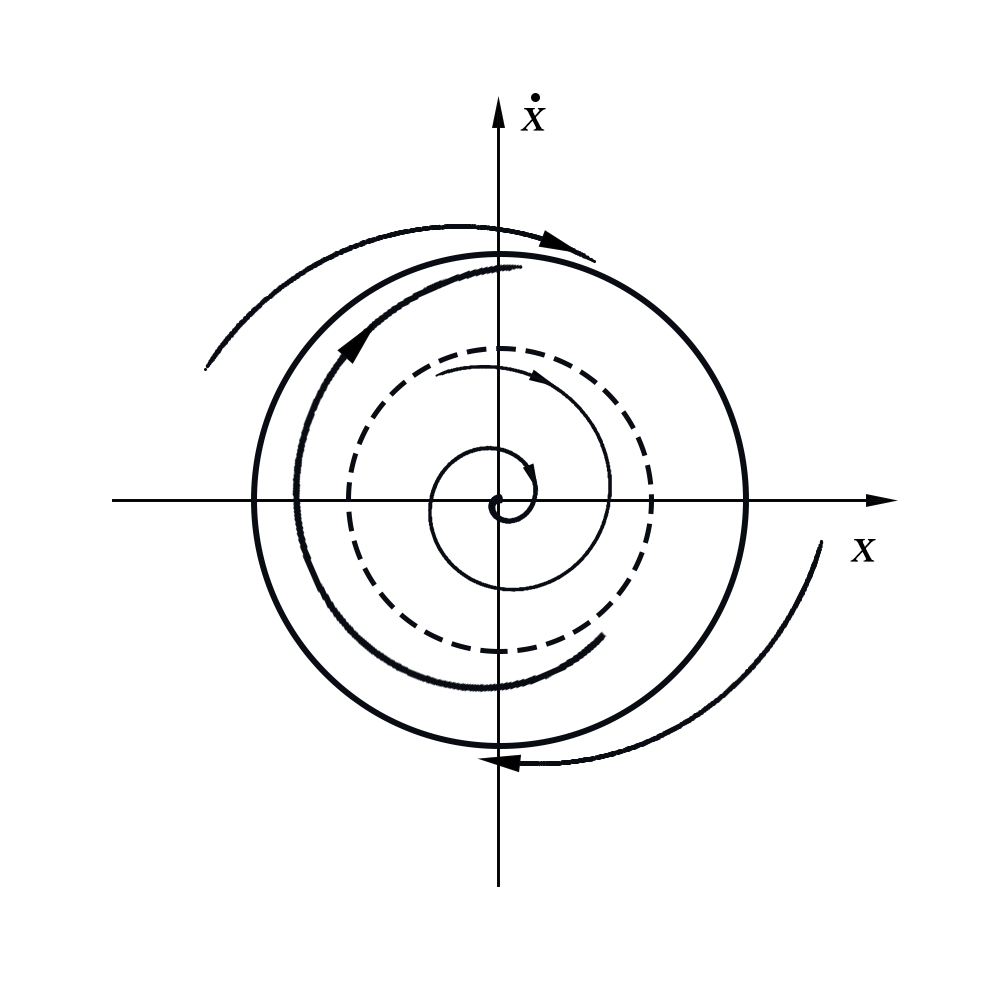
\includegraphics[width=\linewidth]{photo/pics/Ris10b.png}
        \vspace{-30pt}
        \captionof{subfigure}{} 
        \label{fig:11}
    \end{minipage}
    \begin{minipage}{0.32\linewidth}
        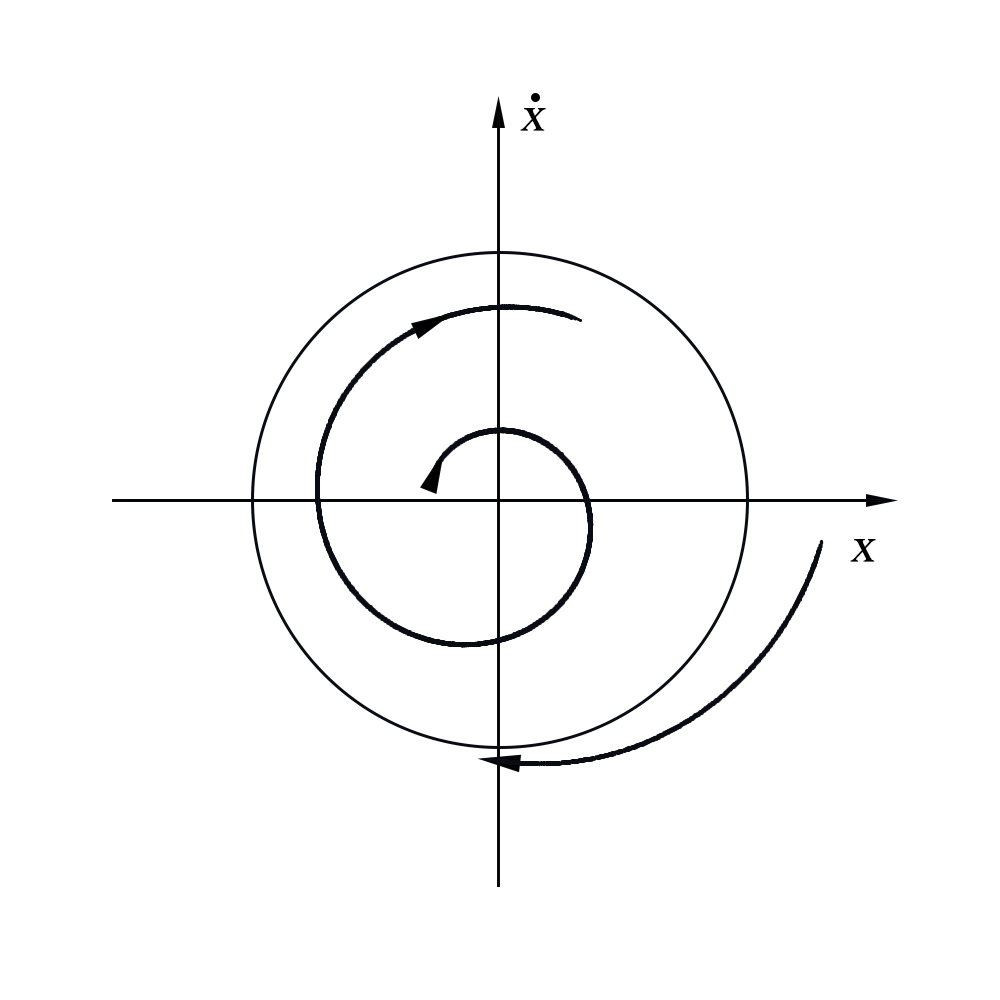
\includegraphics[width=\linewidth]{photo/pics/Ris10c.png}
        \vspace{-30pt}
        \captionof{subfigure}{} 
        \label{fig:12}
    \end{minipage}
    \caption{}
    \vspace{-40pt}
    \end{figure}
\end{center} 
{\bfseries 3.}Если рабочая точка выбрана при положительных напряжениях на сетке лампы, то график нечетной части нелинейной характеристики имеет вид, приведенный на рис.\ref{fig:13}.
\begin{wrapfigure}{r}{.4\linewidth}
    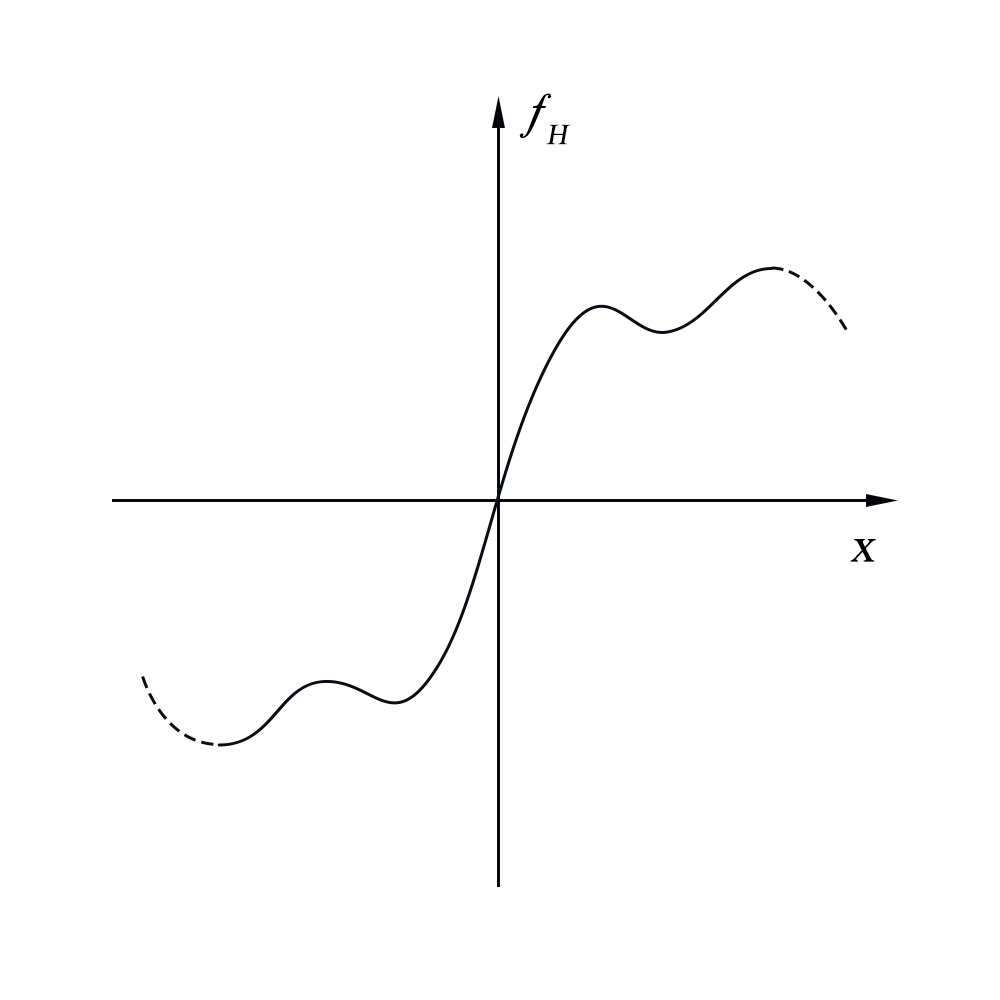
\includegraphics[width=\linewidth]{photo/pics/Ris11.png} 
    \caption{}
    \label{fig:13}
\end{wrapfigure} 

Здесь для аппроксимации анодно-сеточной характеристики лампы необходимо использовать полином седьмой степени. 
В этом случае функция $\bar{f}_1(\rho^2)$ и уравнение для определения ненулевых состояний равновесия запишутся 
в виде $$\bar{f}_1(\rho^2)=a_1+\frac{a_3}{2}\rho^2-\frac{a_5}{12}\rho^4-\frac{a_7}{144}\rho^6,$$ $$\delta-\sigma(a_1+\frac{a_3}{2}\rho^2-\frac{a_5}{12}\rho^4-\frac{a_7}{144}\rho^6)=0.$$
При этом возможны два варианта бифуркационной диаграммы $\bar \rho^2(\sigma)$, изображенные на рис.\ref{fig:16}. 

В варианте a при уменьшении параметра $\sigma$ происходит скачкообразный переход с большего предельного цикла на меньший
 и при дальнейшем уменьшении $\sigma$ предельный цикл плавно исчезает. В варианте b при уменьшении параметра $\sigma$ до $\sigma_0$ колебания срываются до нуля. 

Описанная разновидность автоколебательных систем относится к генераторам {\itshapeсложно-жесткого типа}.
\begin{center}
    \begin{figure}[h!]
        \vspace{-10pt}
        \begin{minipage}{0.49\linewidth}
            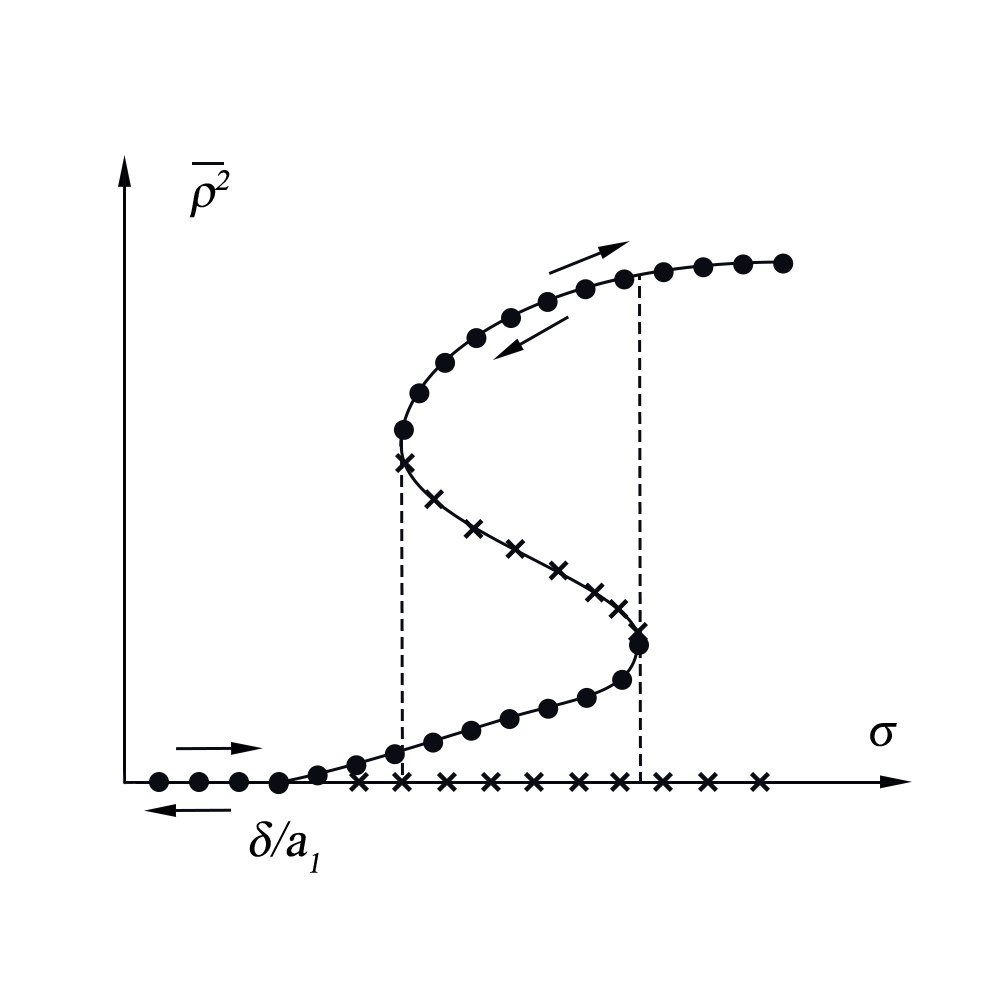
\includegraphics[width=\linewidth]{photo/pics/Ris12a.png} 
            \vspace{-50pt}
            \label{fig:14}
            \captionof{subfigure}{} 
        \end{minipage}
    \begin{minipage}{0.49\linewidth}
        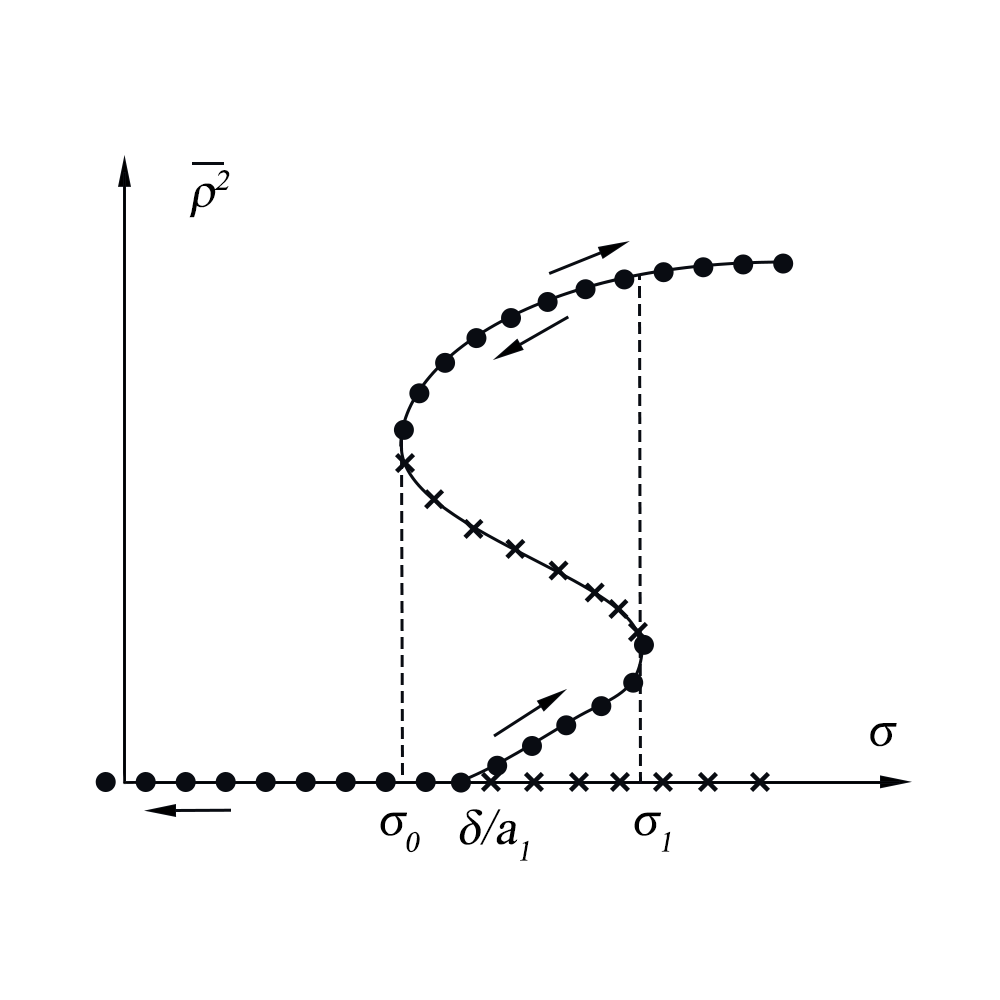
\includegraphics[width=\linewidth]{photo/pics/Ris12b.png} 
        \vspace{-50pt}
        \label{fig:15}
        \captionof{subfigure}{} 
    \end{minipage}
    \caption{}
    \label{fig:16}
    \vspace{-40pt}
    \end{figure}
\end{center} 

\newpage
\section{Эксперимент}
На рис.\ref{fig1} представлена схема установки.
\begin{figure}[h]
	\centering
	\vspace{-10pt}
	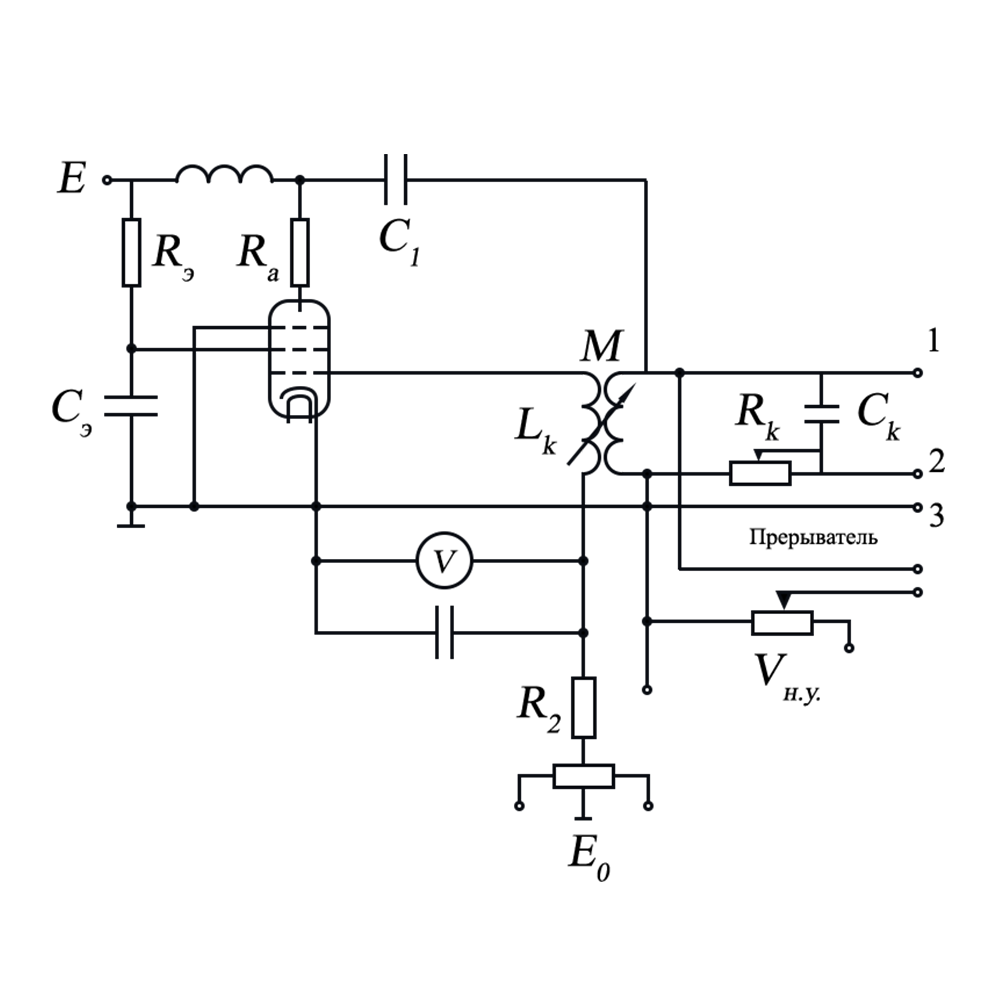
\includegraphics[width=0.35\linewidth]{photo/pics/scheme.png}
	\vspace{-20pt}
	\caption{схема установки}
	\label{fig1}
\end{figure}
\subsection{Мягкий режим генератора}
Подбирая напряжения смещения $E_0$, добились мягкого режима работы генератора.
\subsubsection{Бифрукационная диаграмма}
Сняли бифуркационную диаграмму, выражающую зависимость амплитуды автоколебаний от величины взаимоиндукции $M$.
\begin{figure}[h]
	\centering
	\vspace{-10pt}
	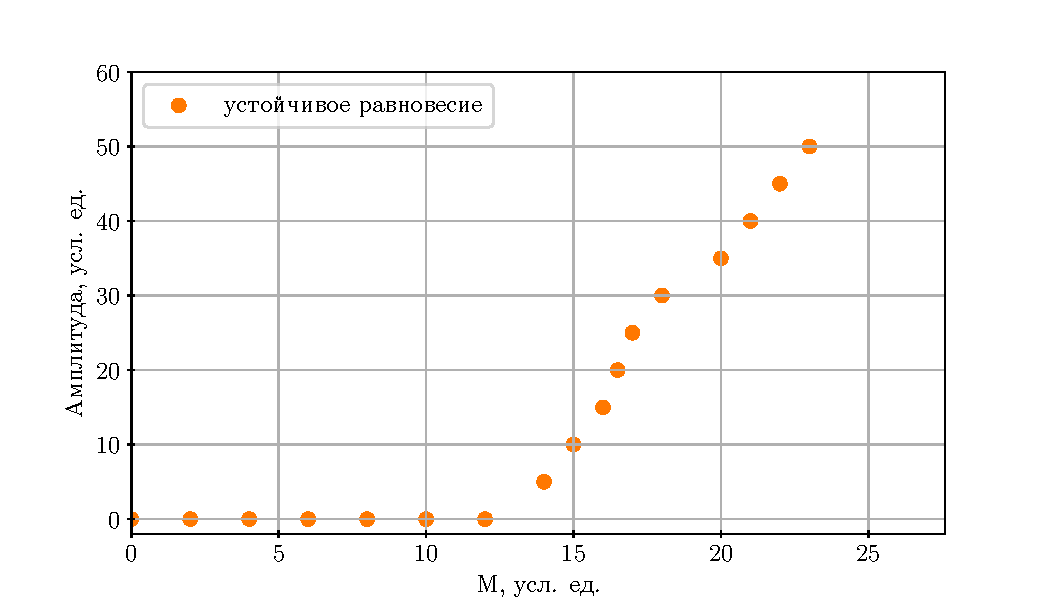
\includegraphics[]{plots/softdiagram.pdf}
	\caption{бифрукационная диаграмма для мягкого режима}
	\label{fig2}
\end{figure}
По графику можно наблюдать характерную кривую бифрукационной диаграммы для мягкого режима генератора.
\subsubsection{Фазовые траектории}
Получили фазовые траектории при различных начальных условиях для качественно различного поведения системы (левее и правее точки бифуркации).
\begin{figure}[h]
	\centering
	\begin{minipage}{0.32\linewidth}
	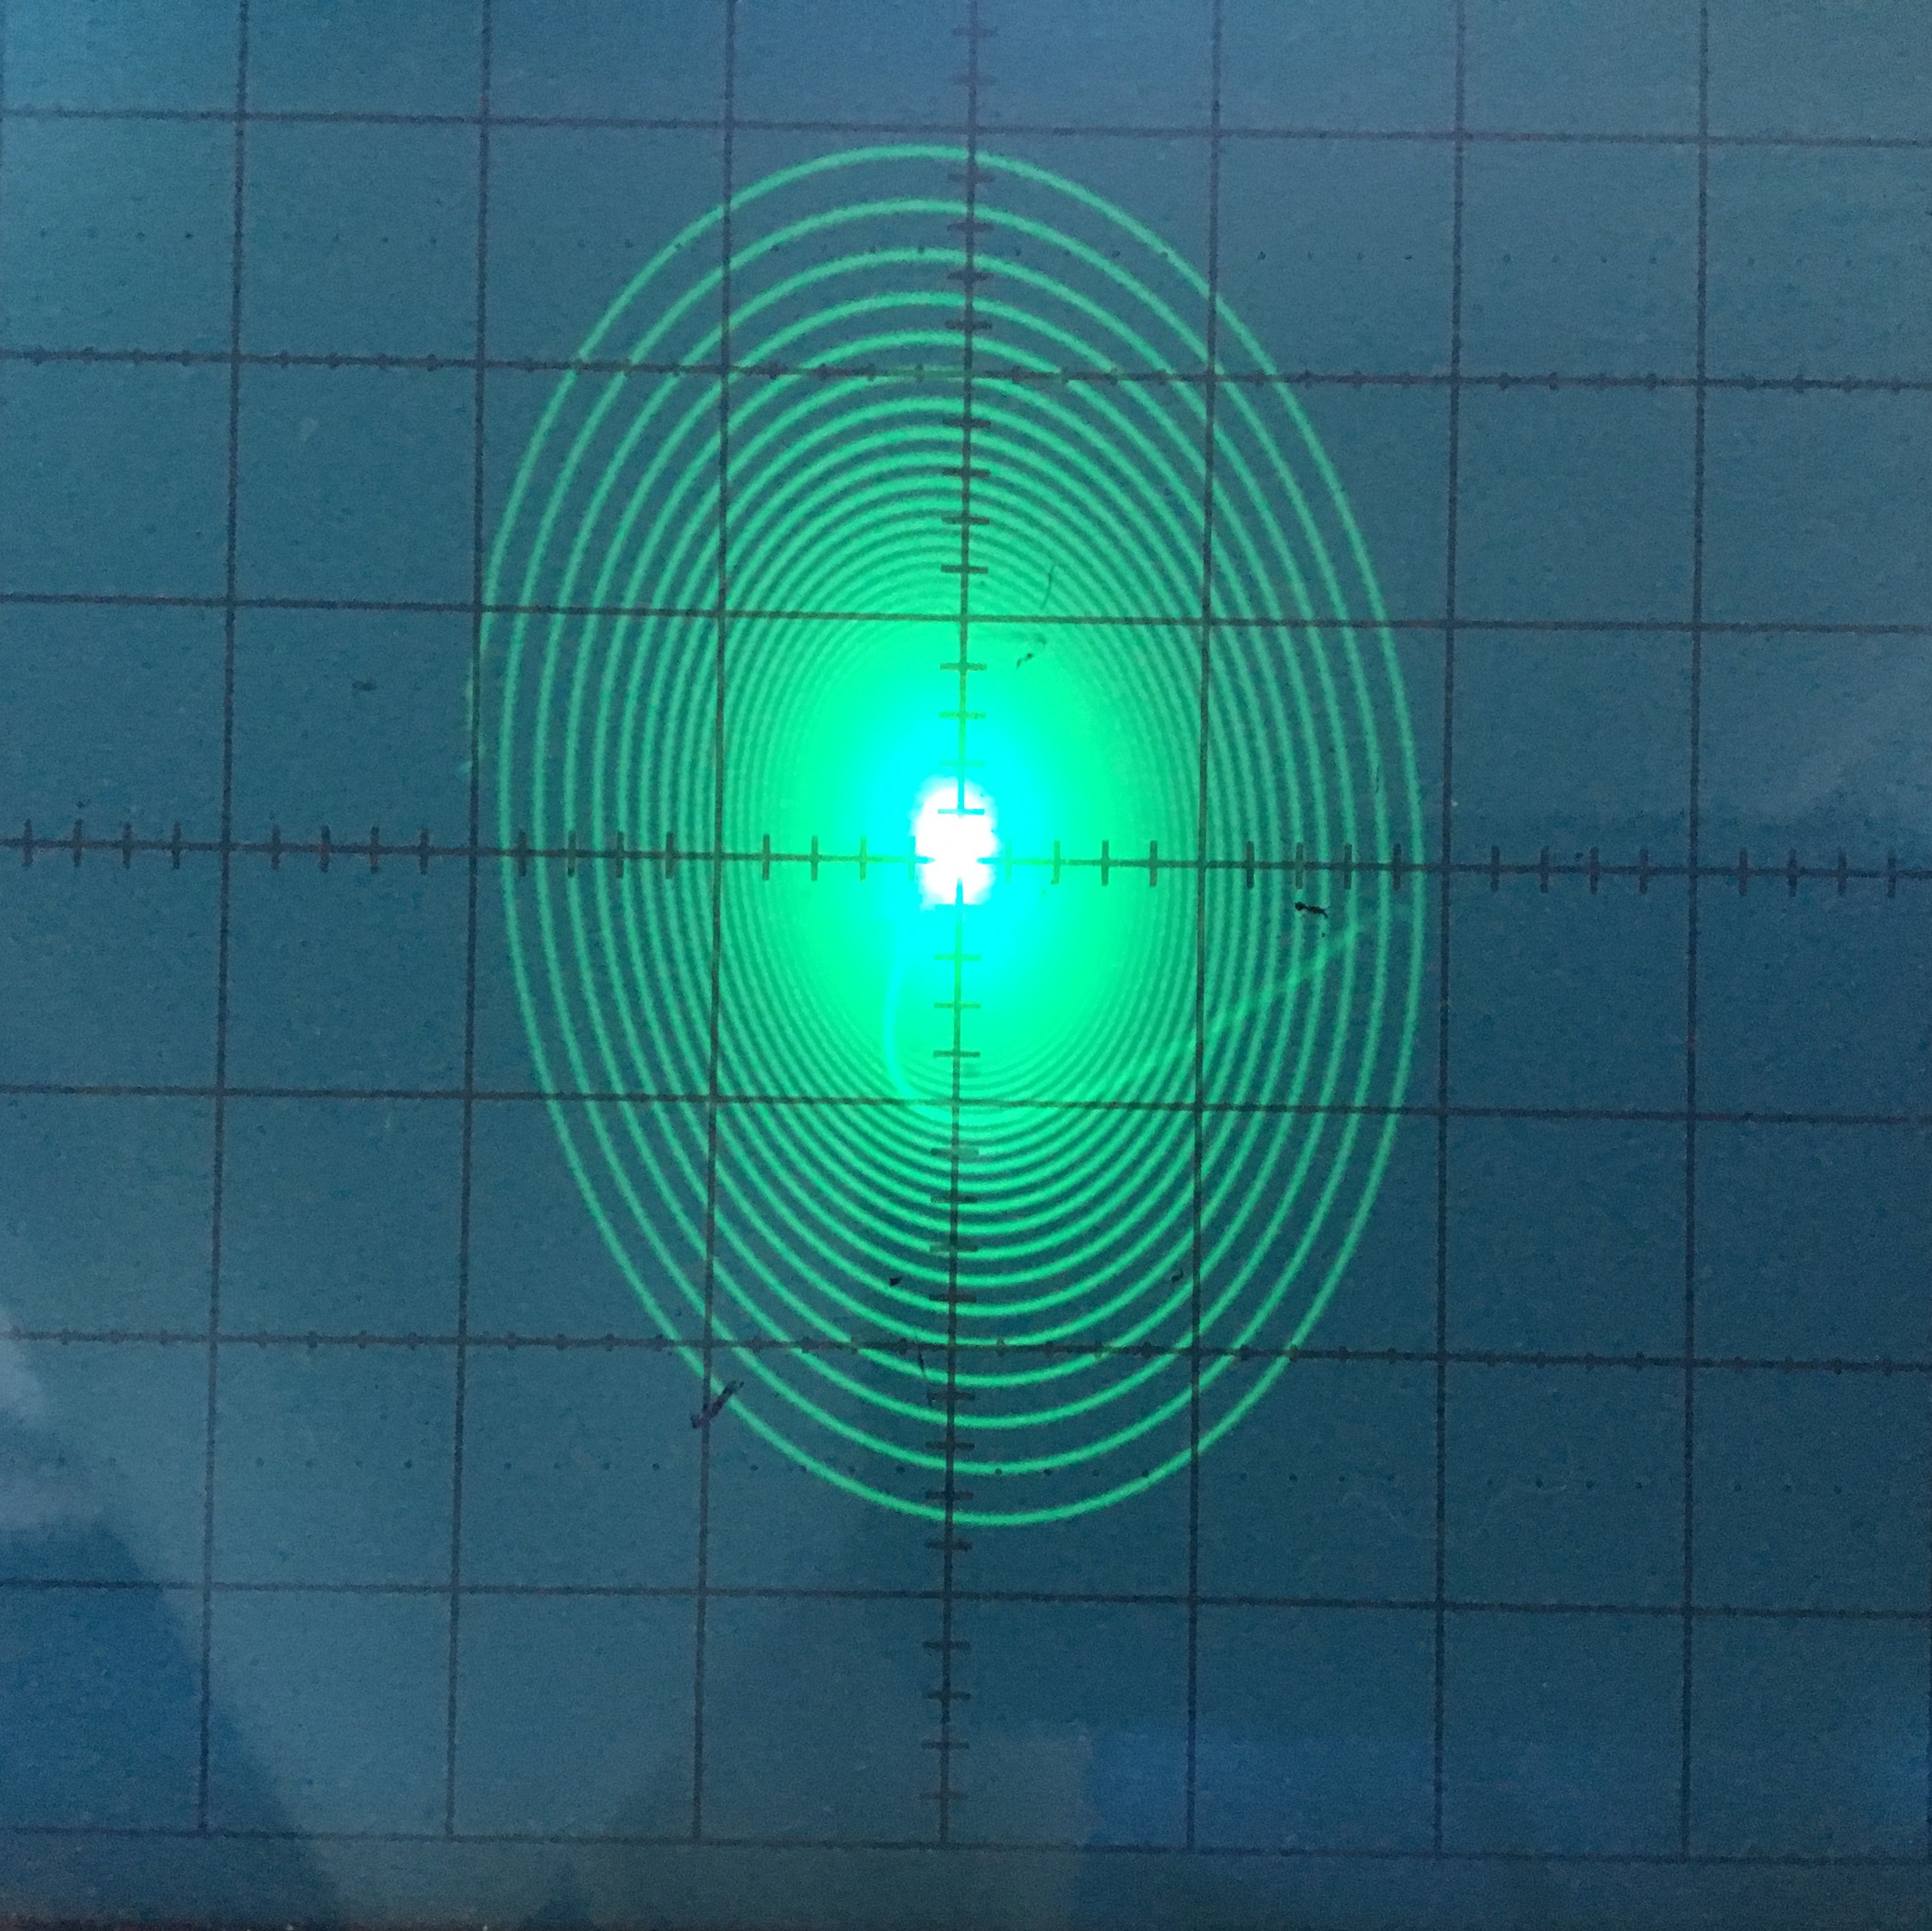
\includegraphics[width=\linewidth]{photo/task1b(lefts).jpg}
	\end{minipage}
	\begin{minipage}{0.32\linewidth}
	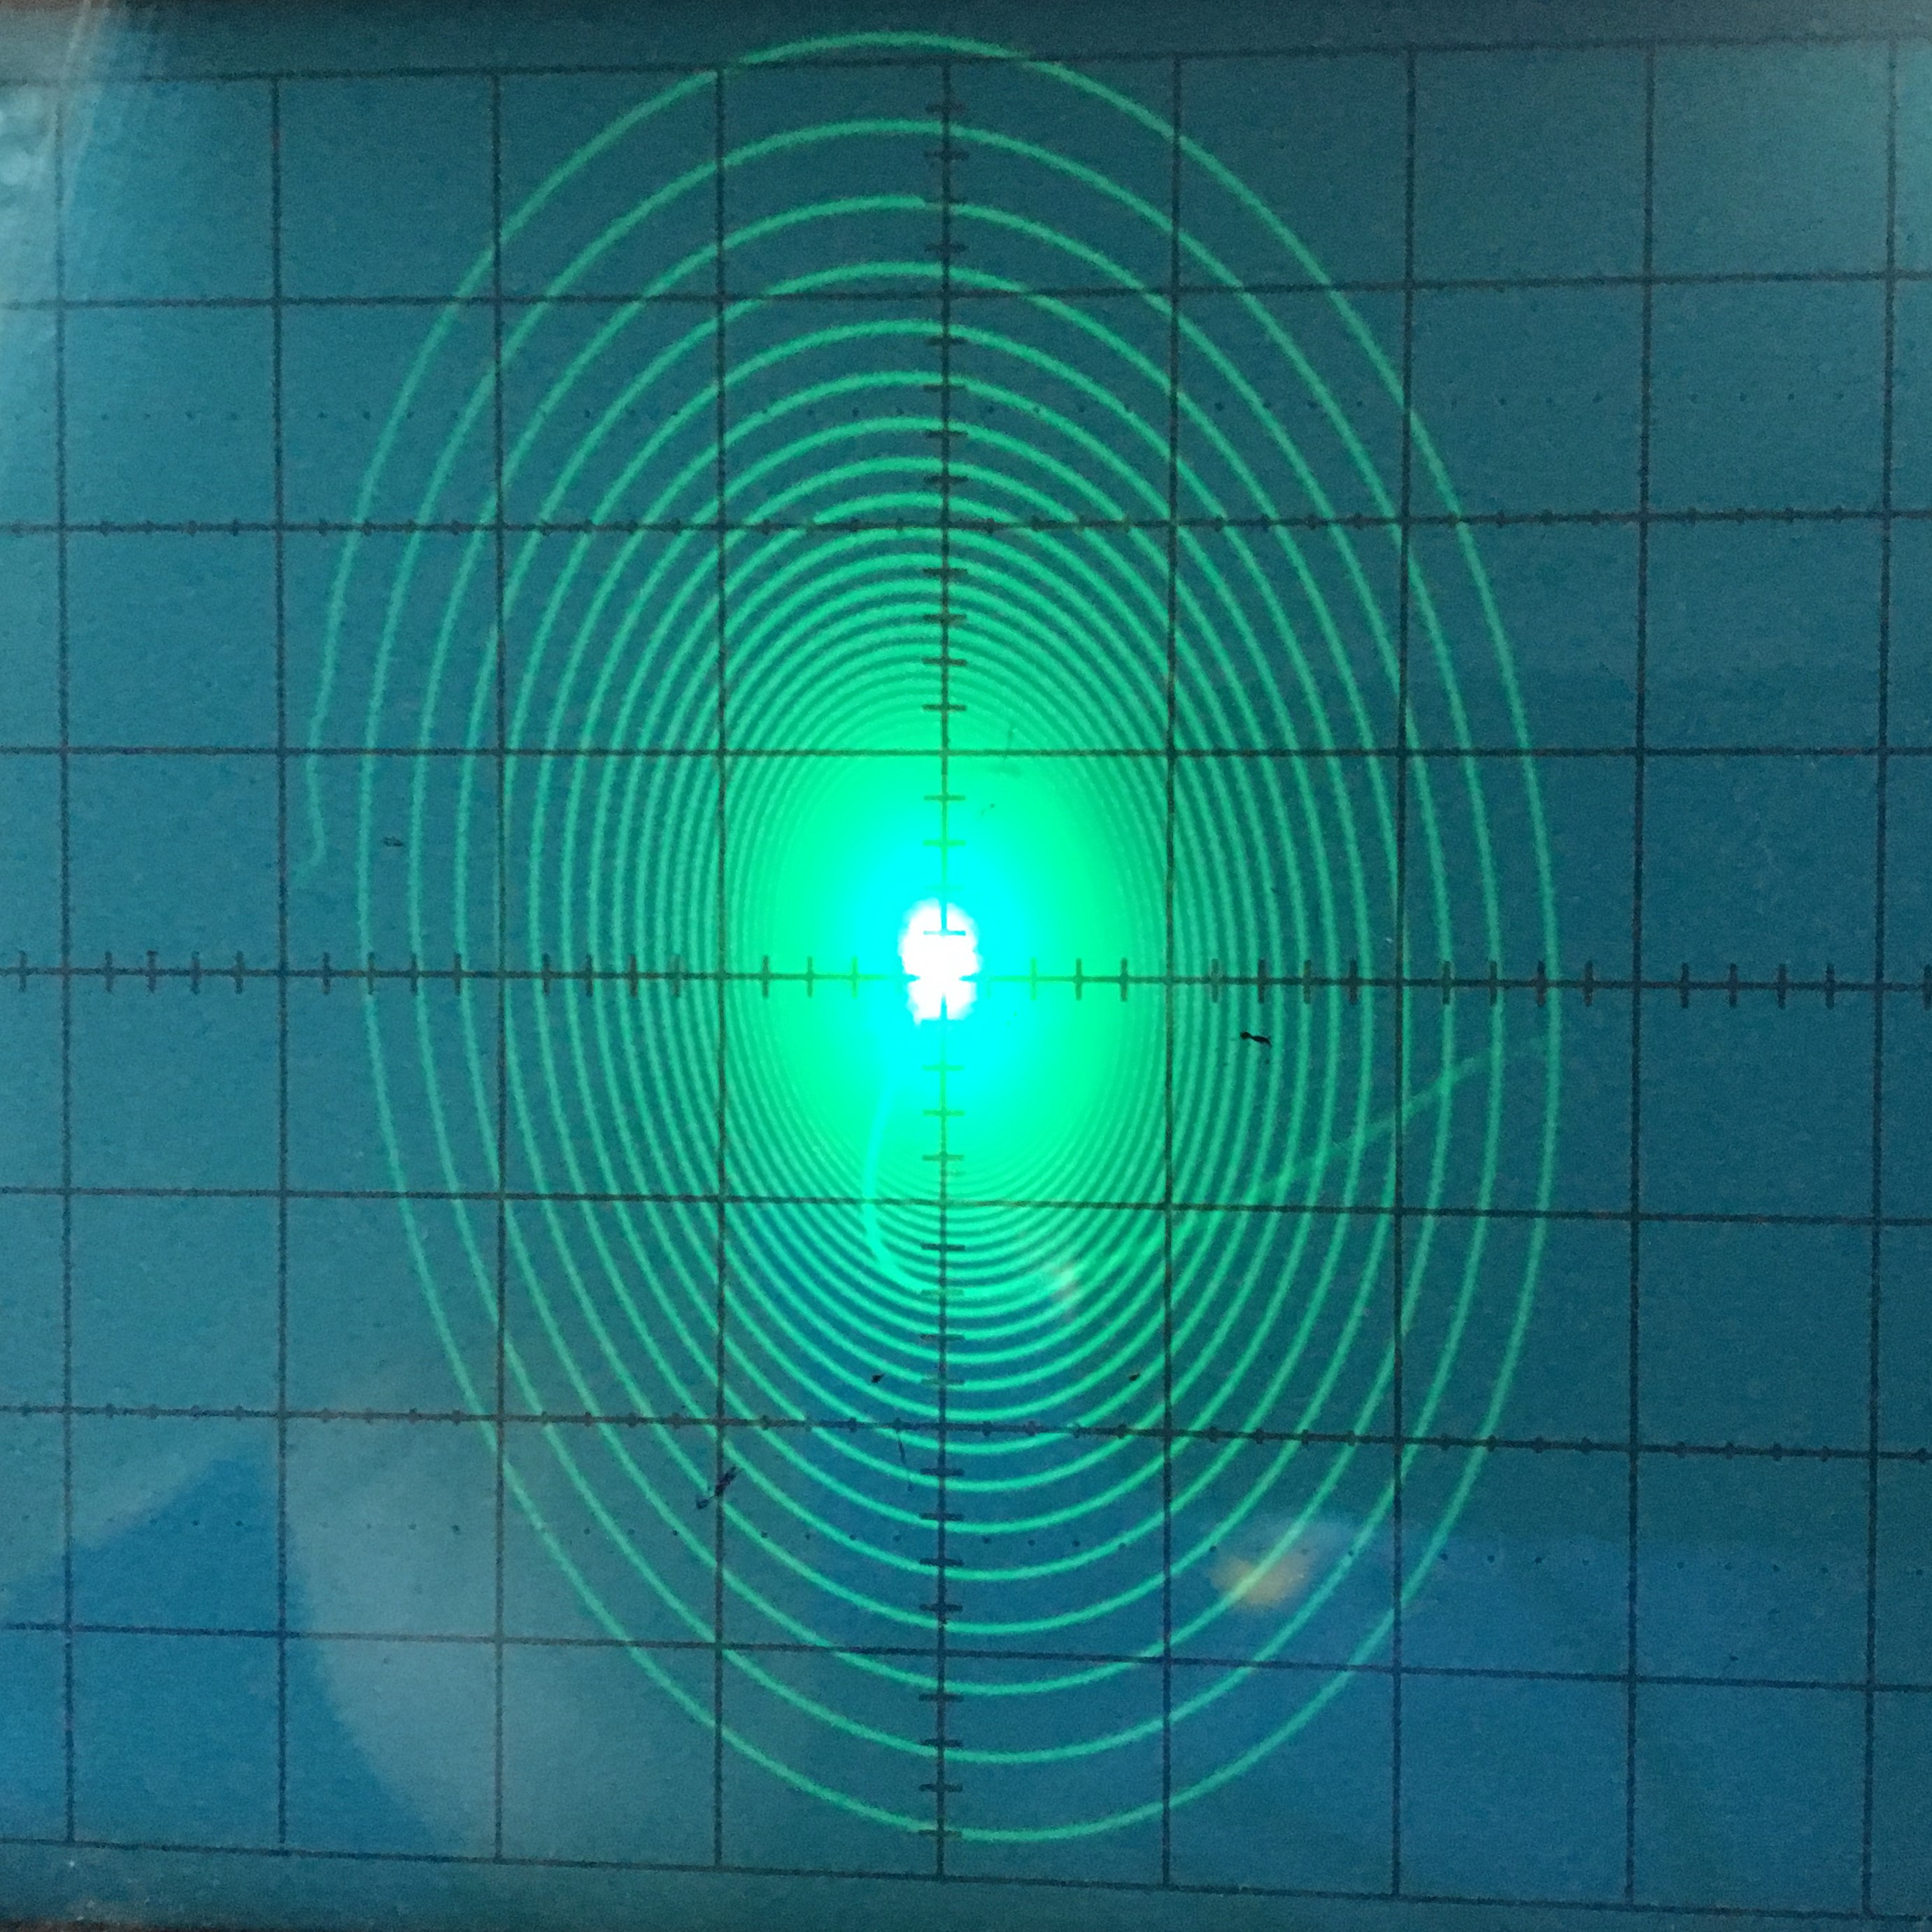
\includegraphics[width=\linewidth]{photo/task1b(leftm).jpg}
	\end{minipage}
	\begin{minipage}{0.32\linewidth}
	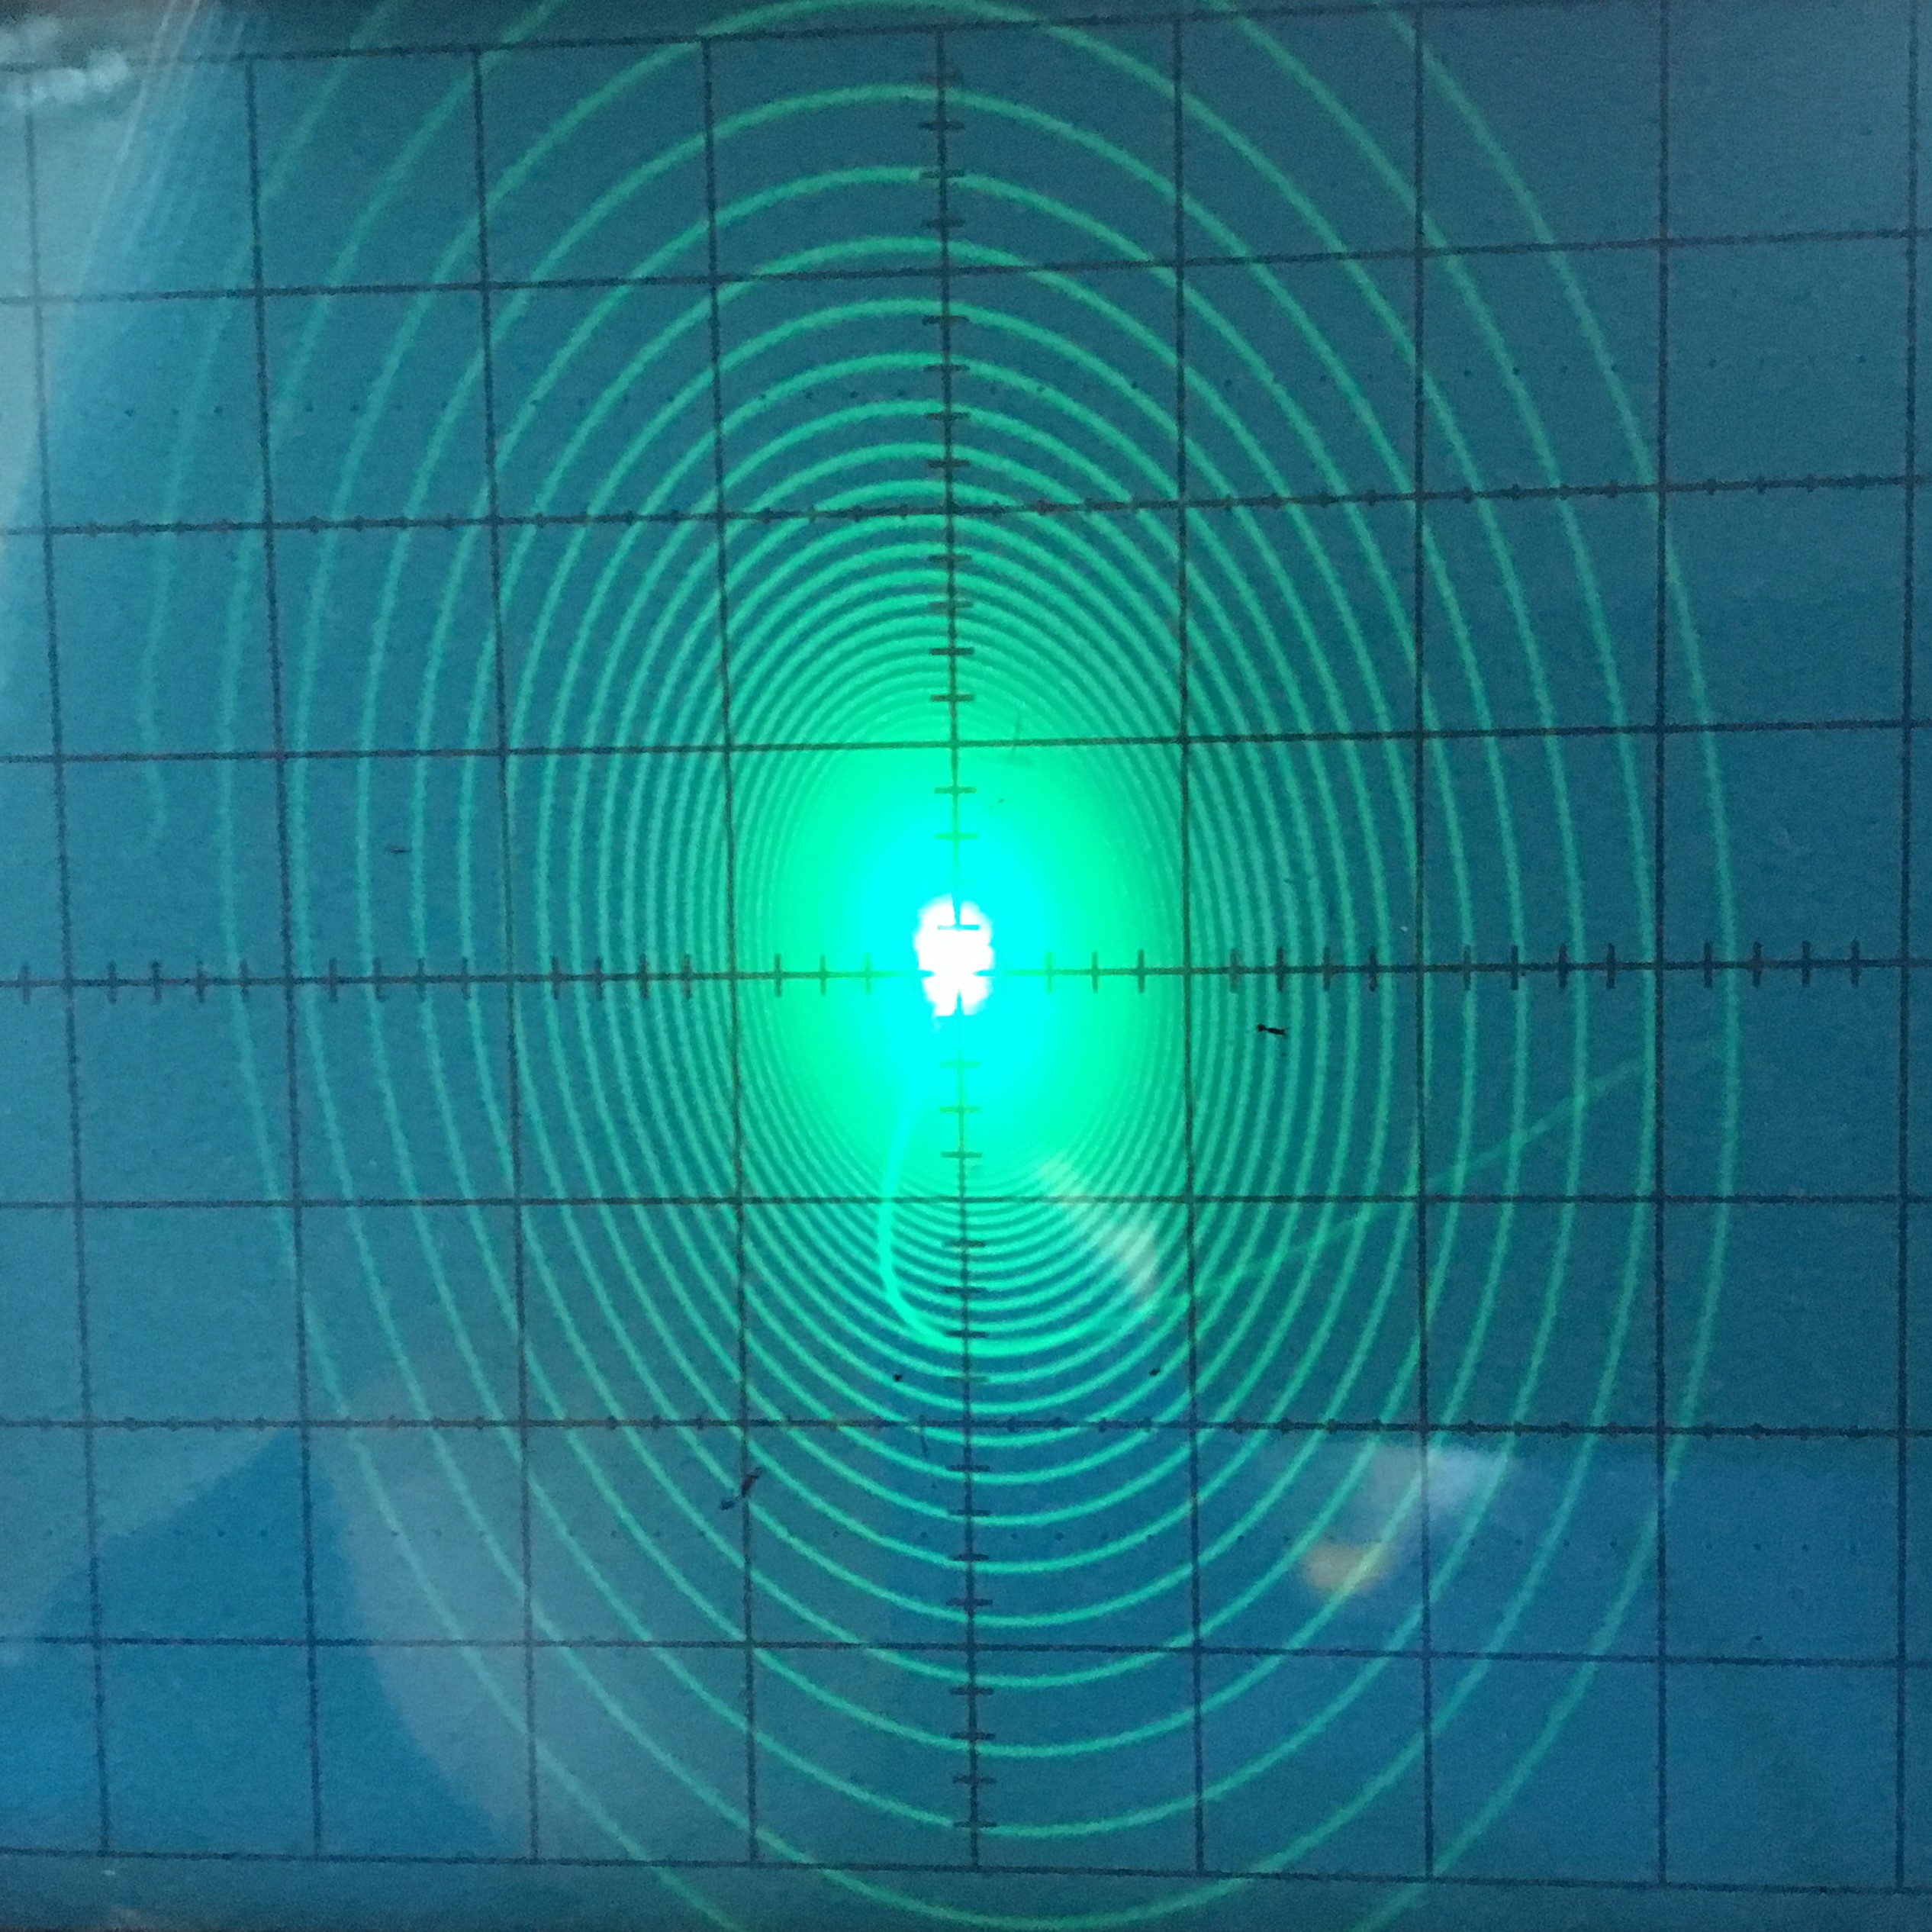
\includegraphics[width=\linewidth]{photo/task1b(leftL).jpg}
	\end{minipage}
	\caption{Левее точки бифрукации}
	\label{fig3}
\end{figure}
По фазовым траекториям видно, что устойчивый режим наблюдается в нуле, так как мы находимся левее точки бифрукации.
\begin{figure}[h]
	\centering
	\begin{minipage}{0.32\linewidth}
	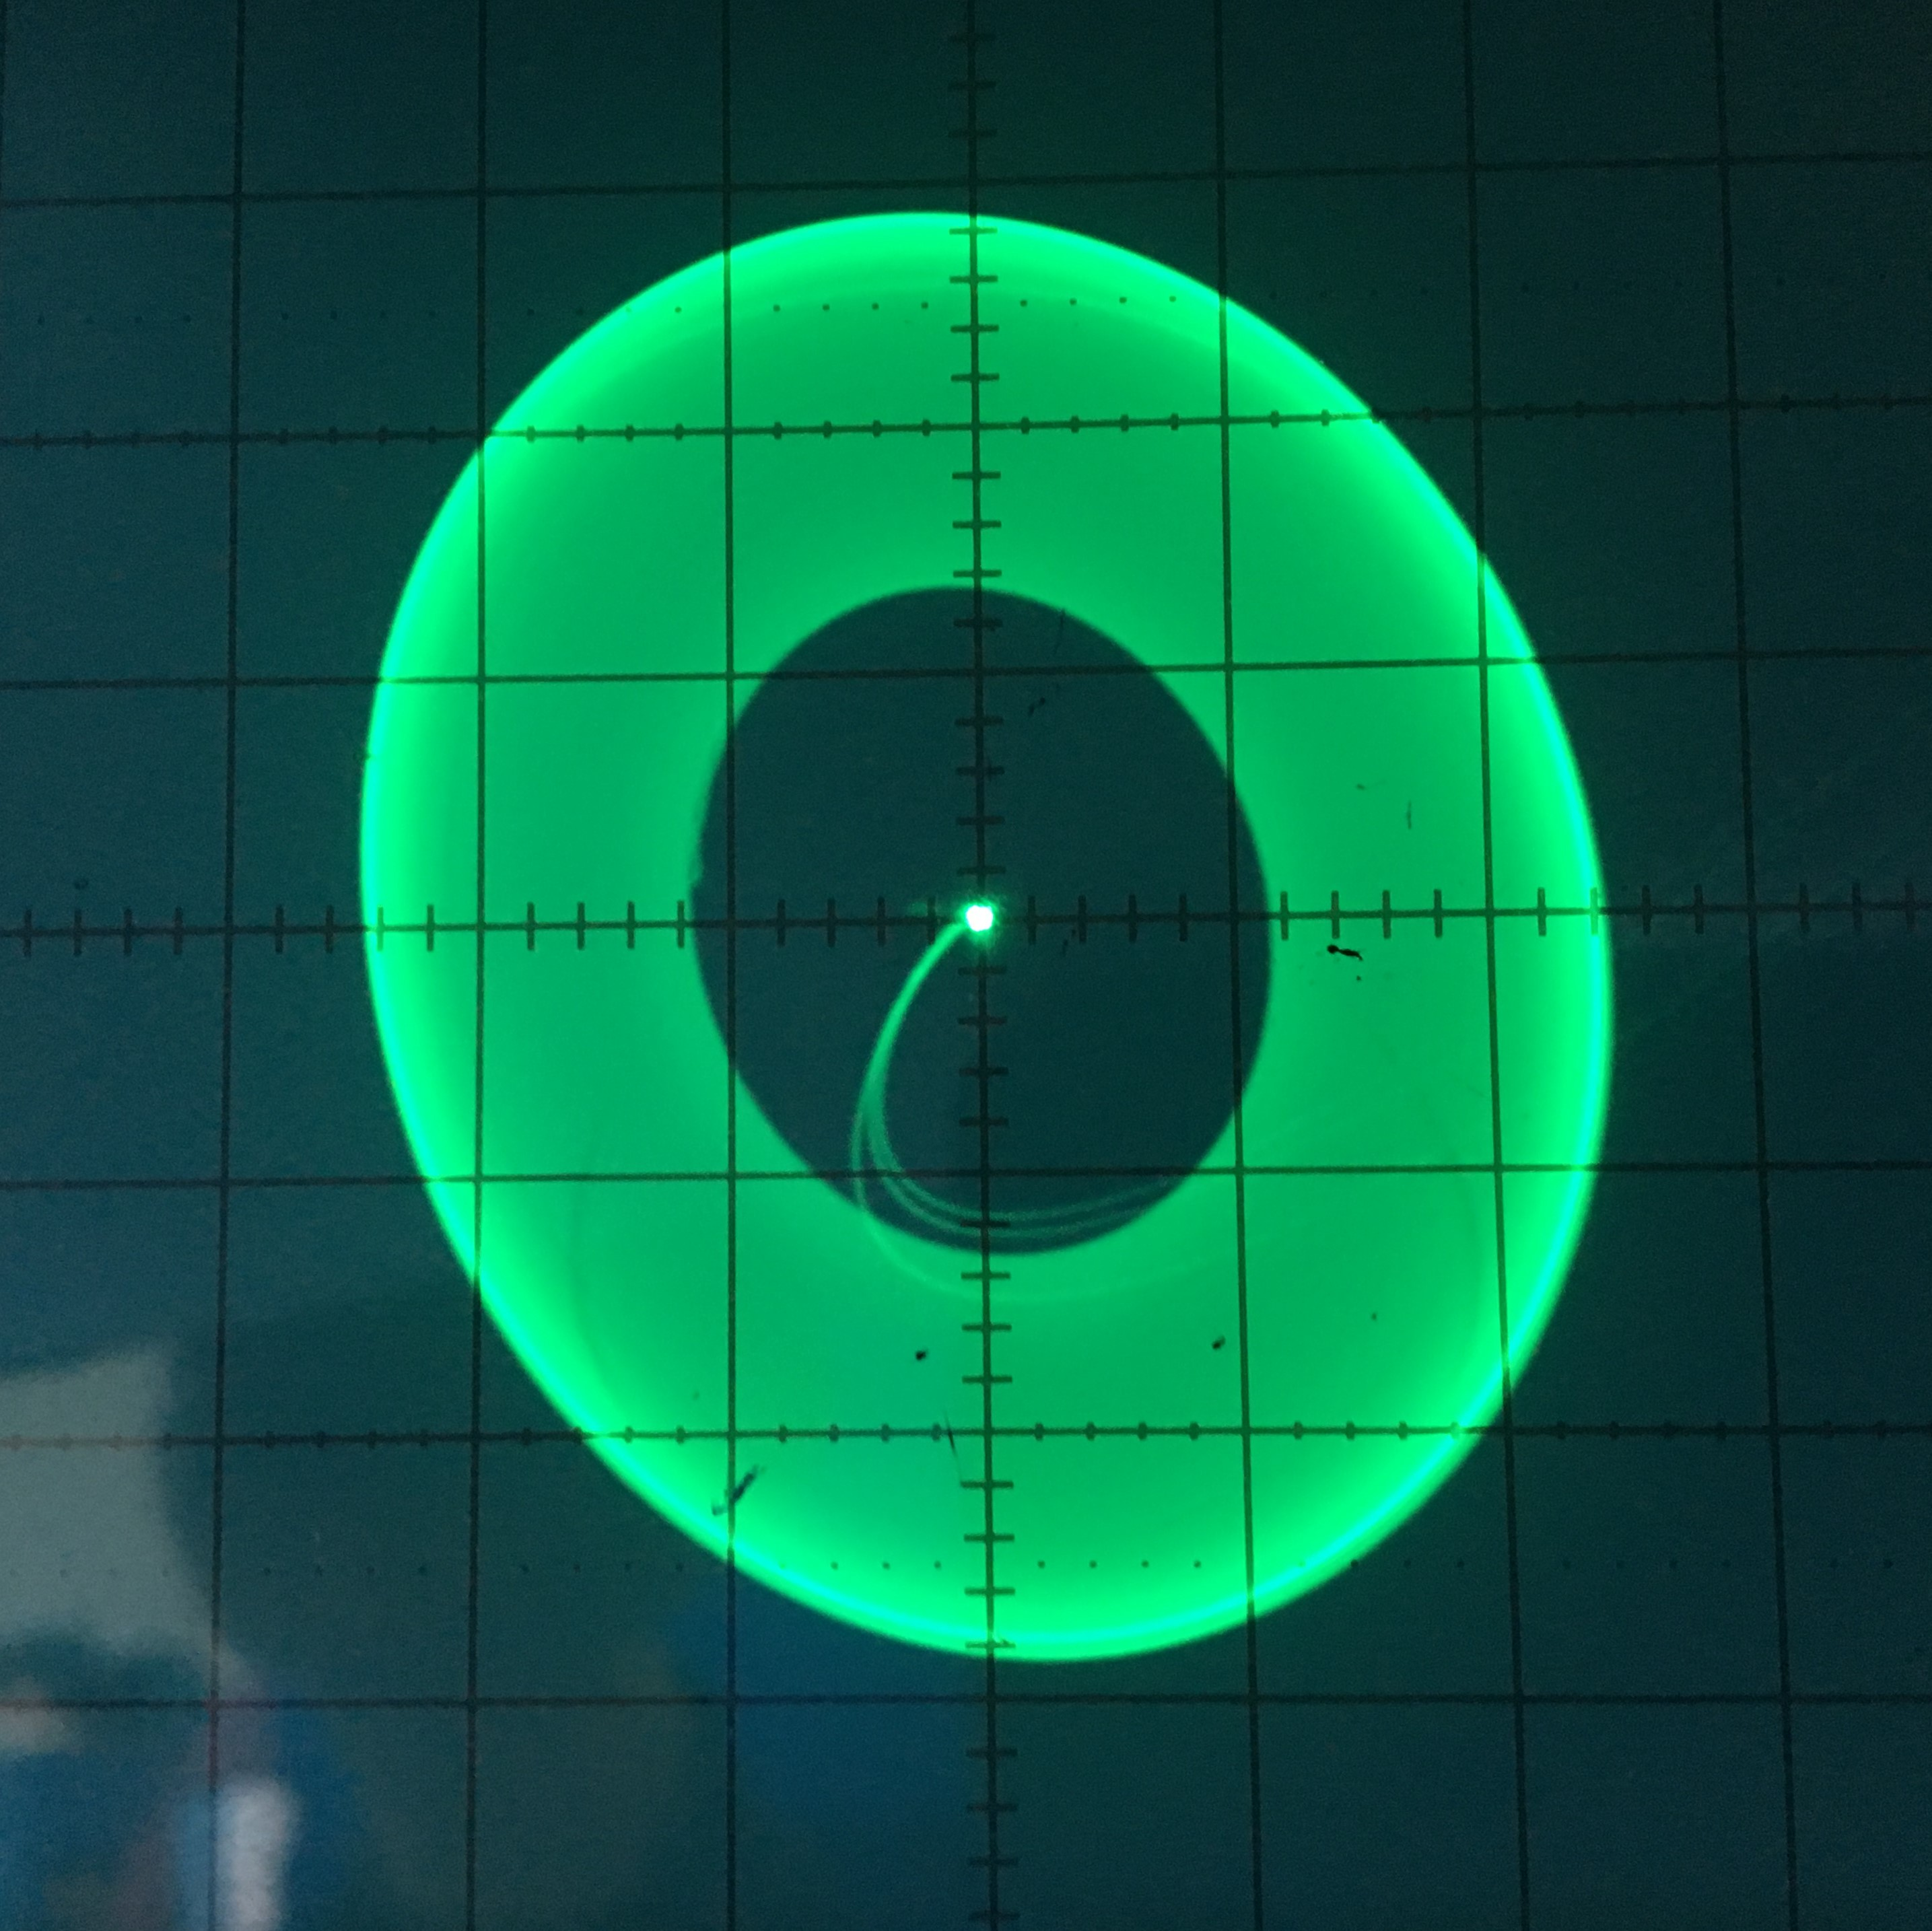
\includegraphics[width=\linewidth]{photo/task1b(rights2).jpg}
	\end{minipage}
	\begin{minipage}{0.32\linewidth}
	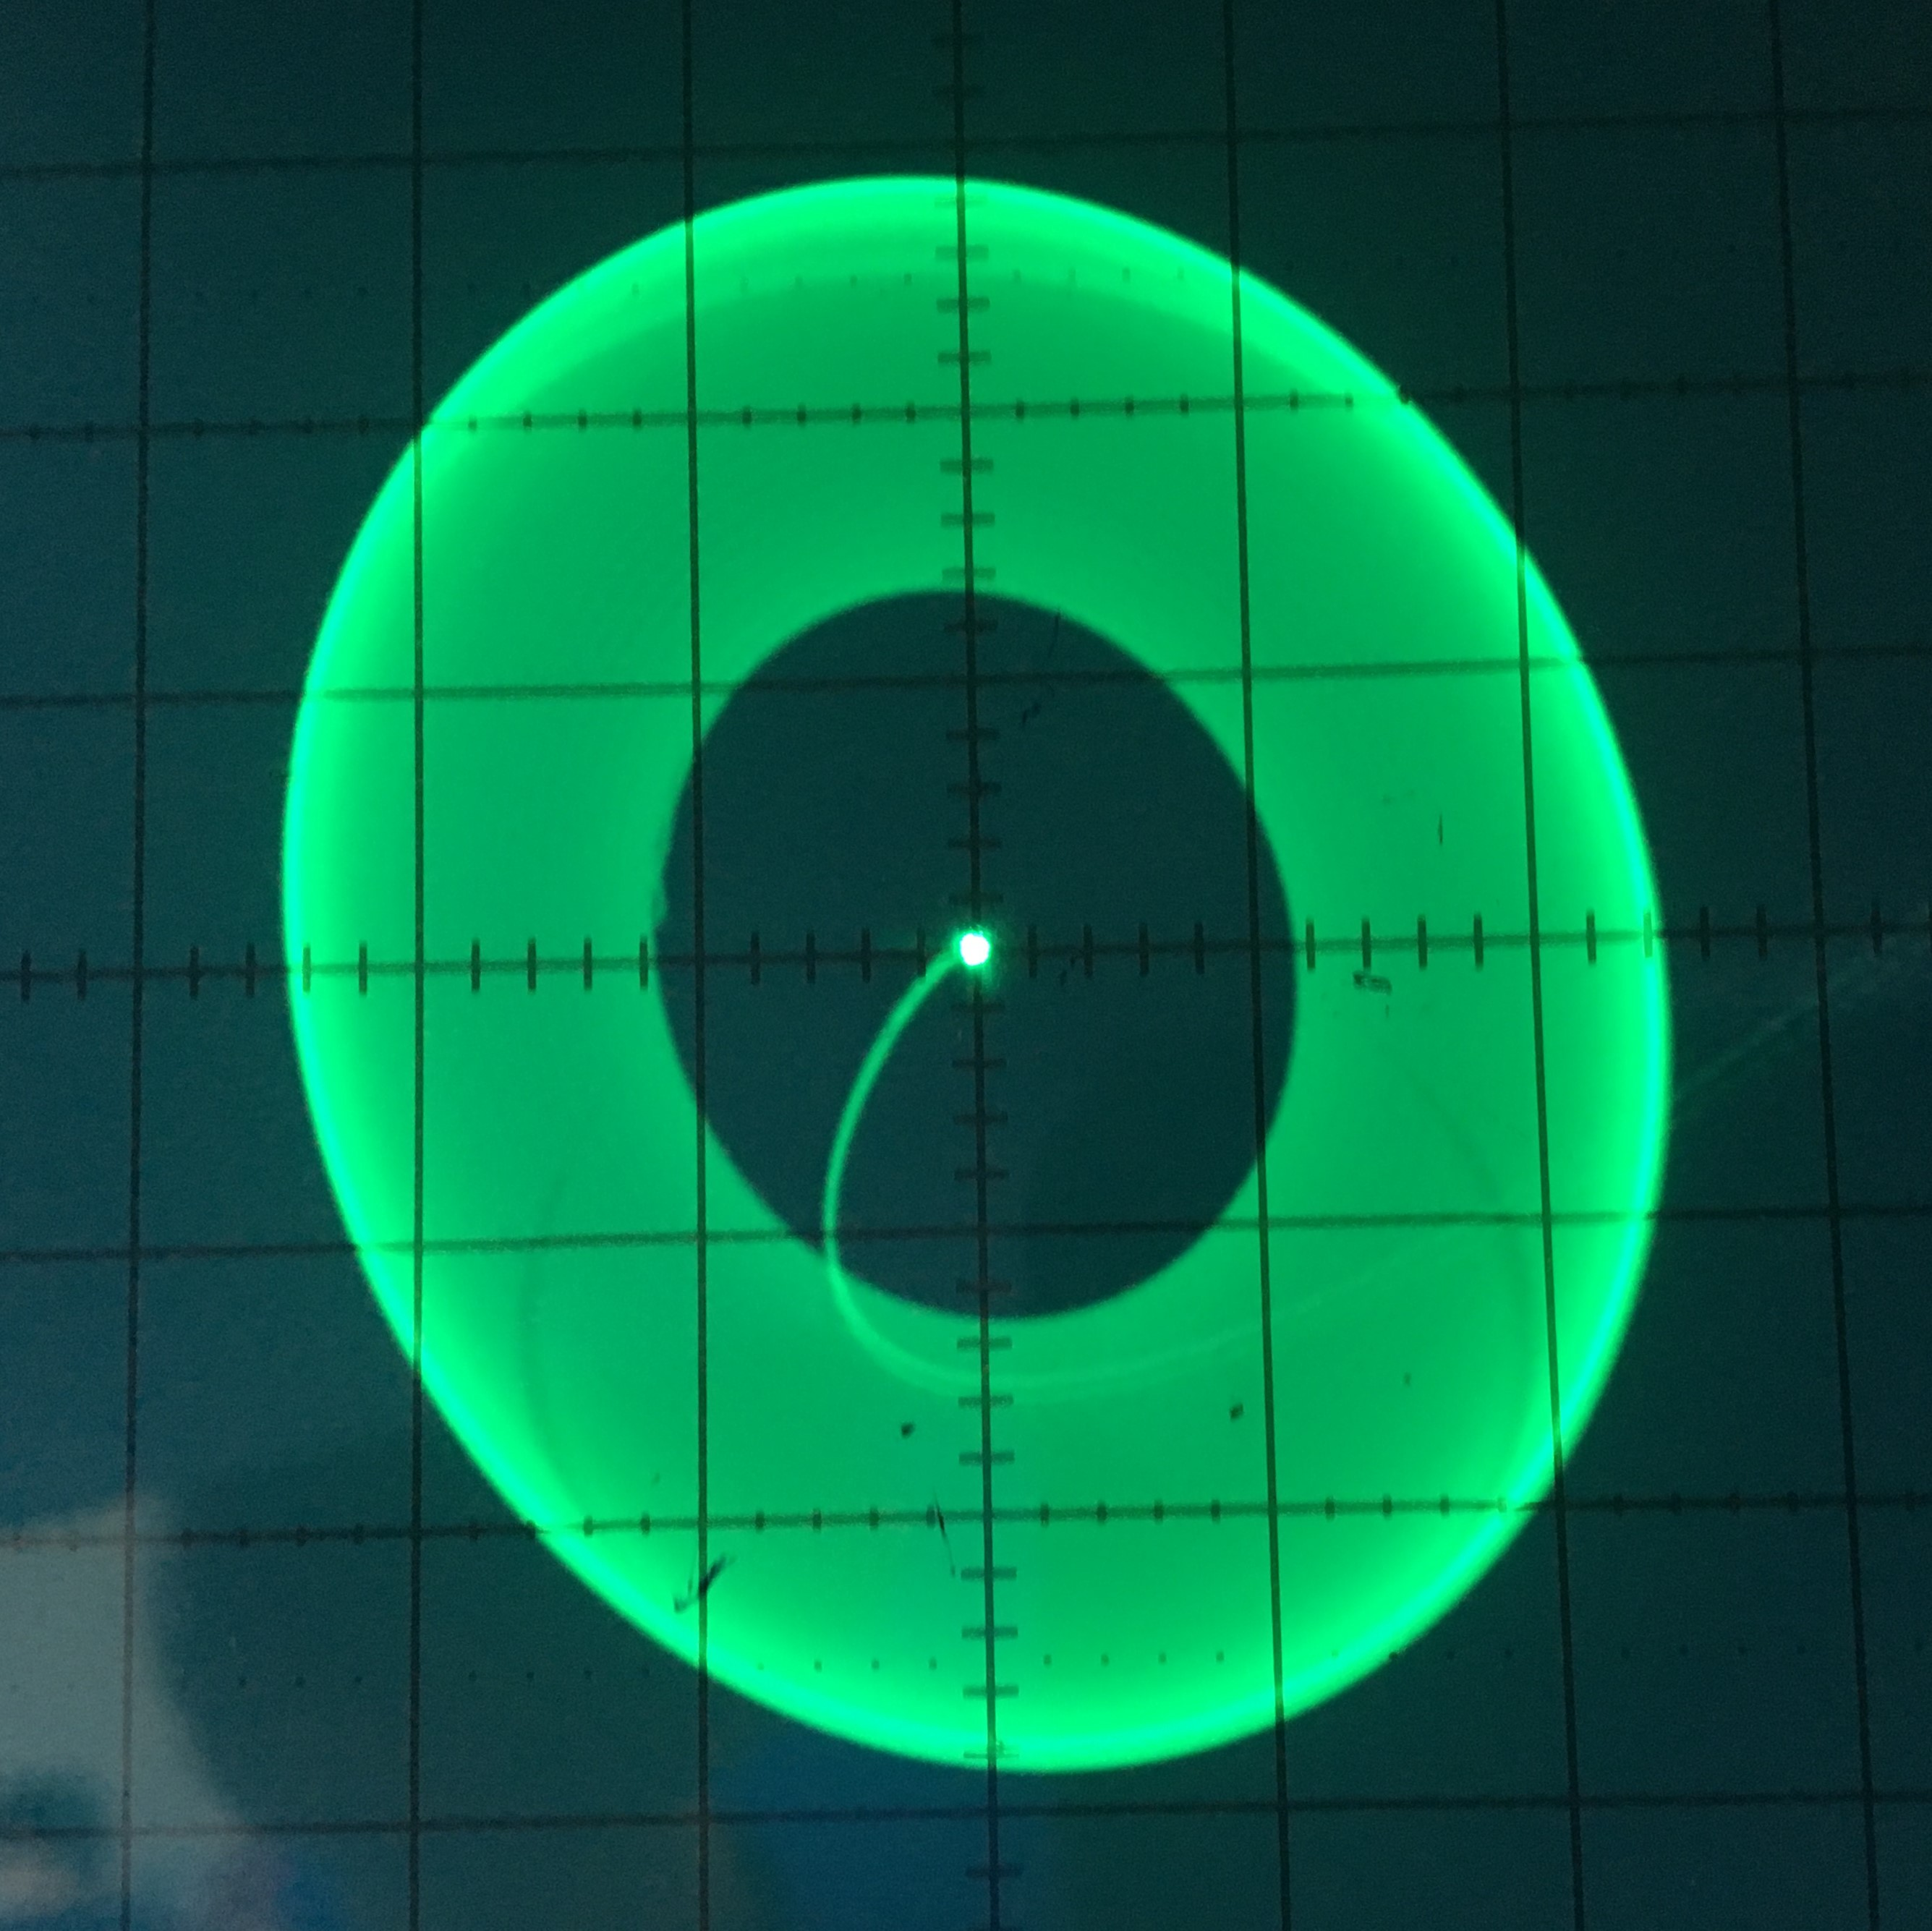
\includegraphics[width=\linewidth]{photo/task1b(rights).jpg}
	\end{minipage}
	\begin{minipage}{0.32\linewidth}
	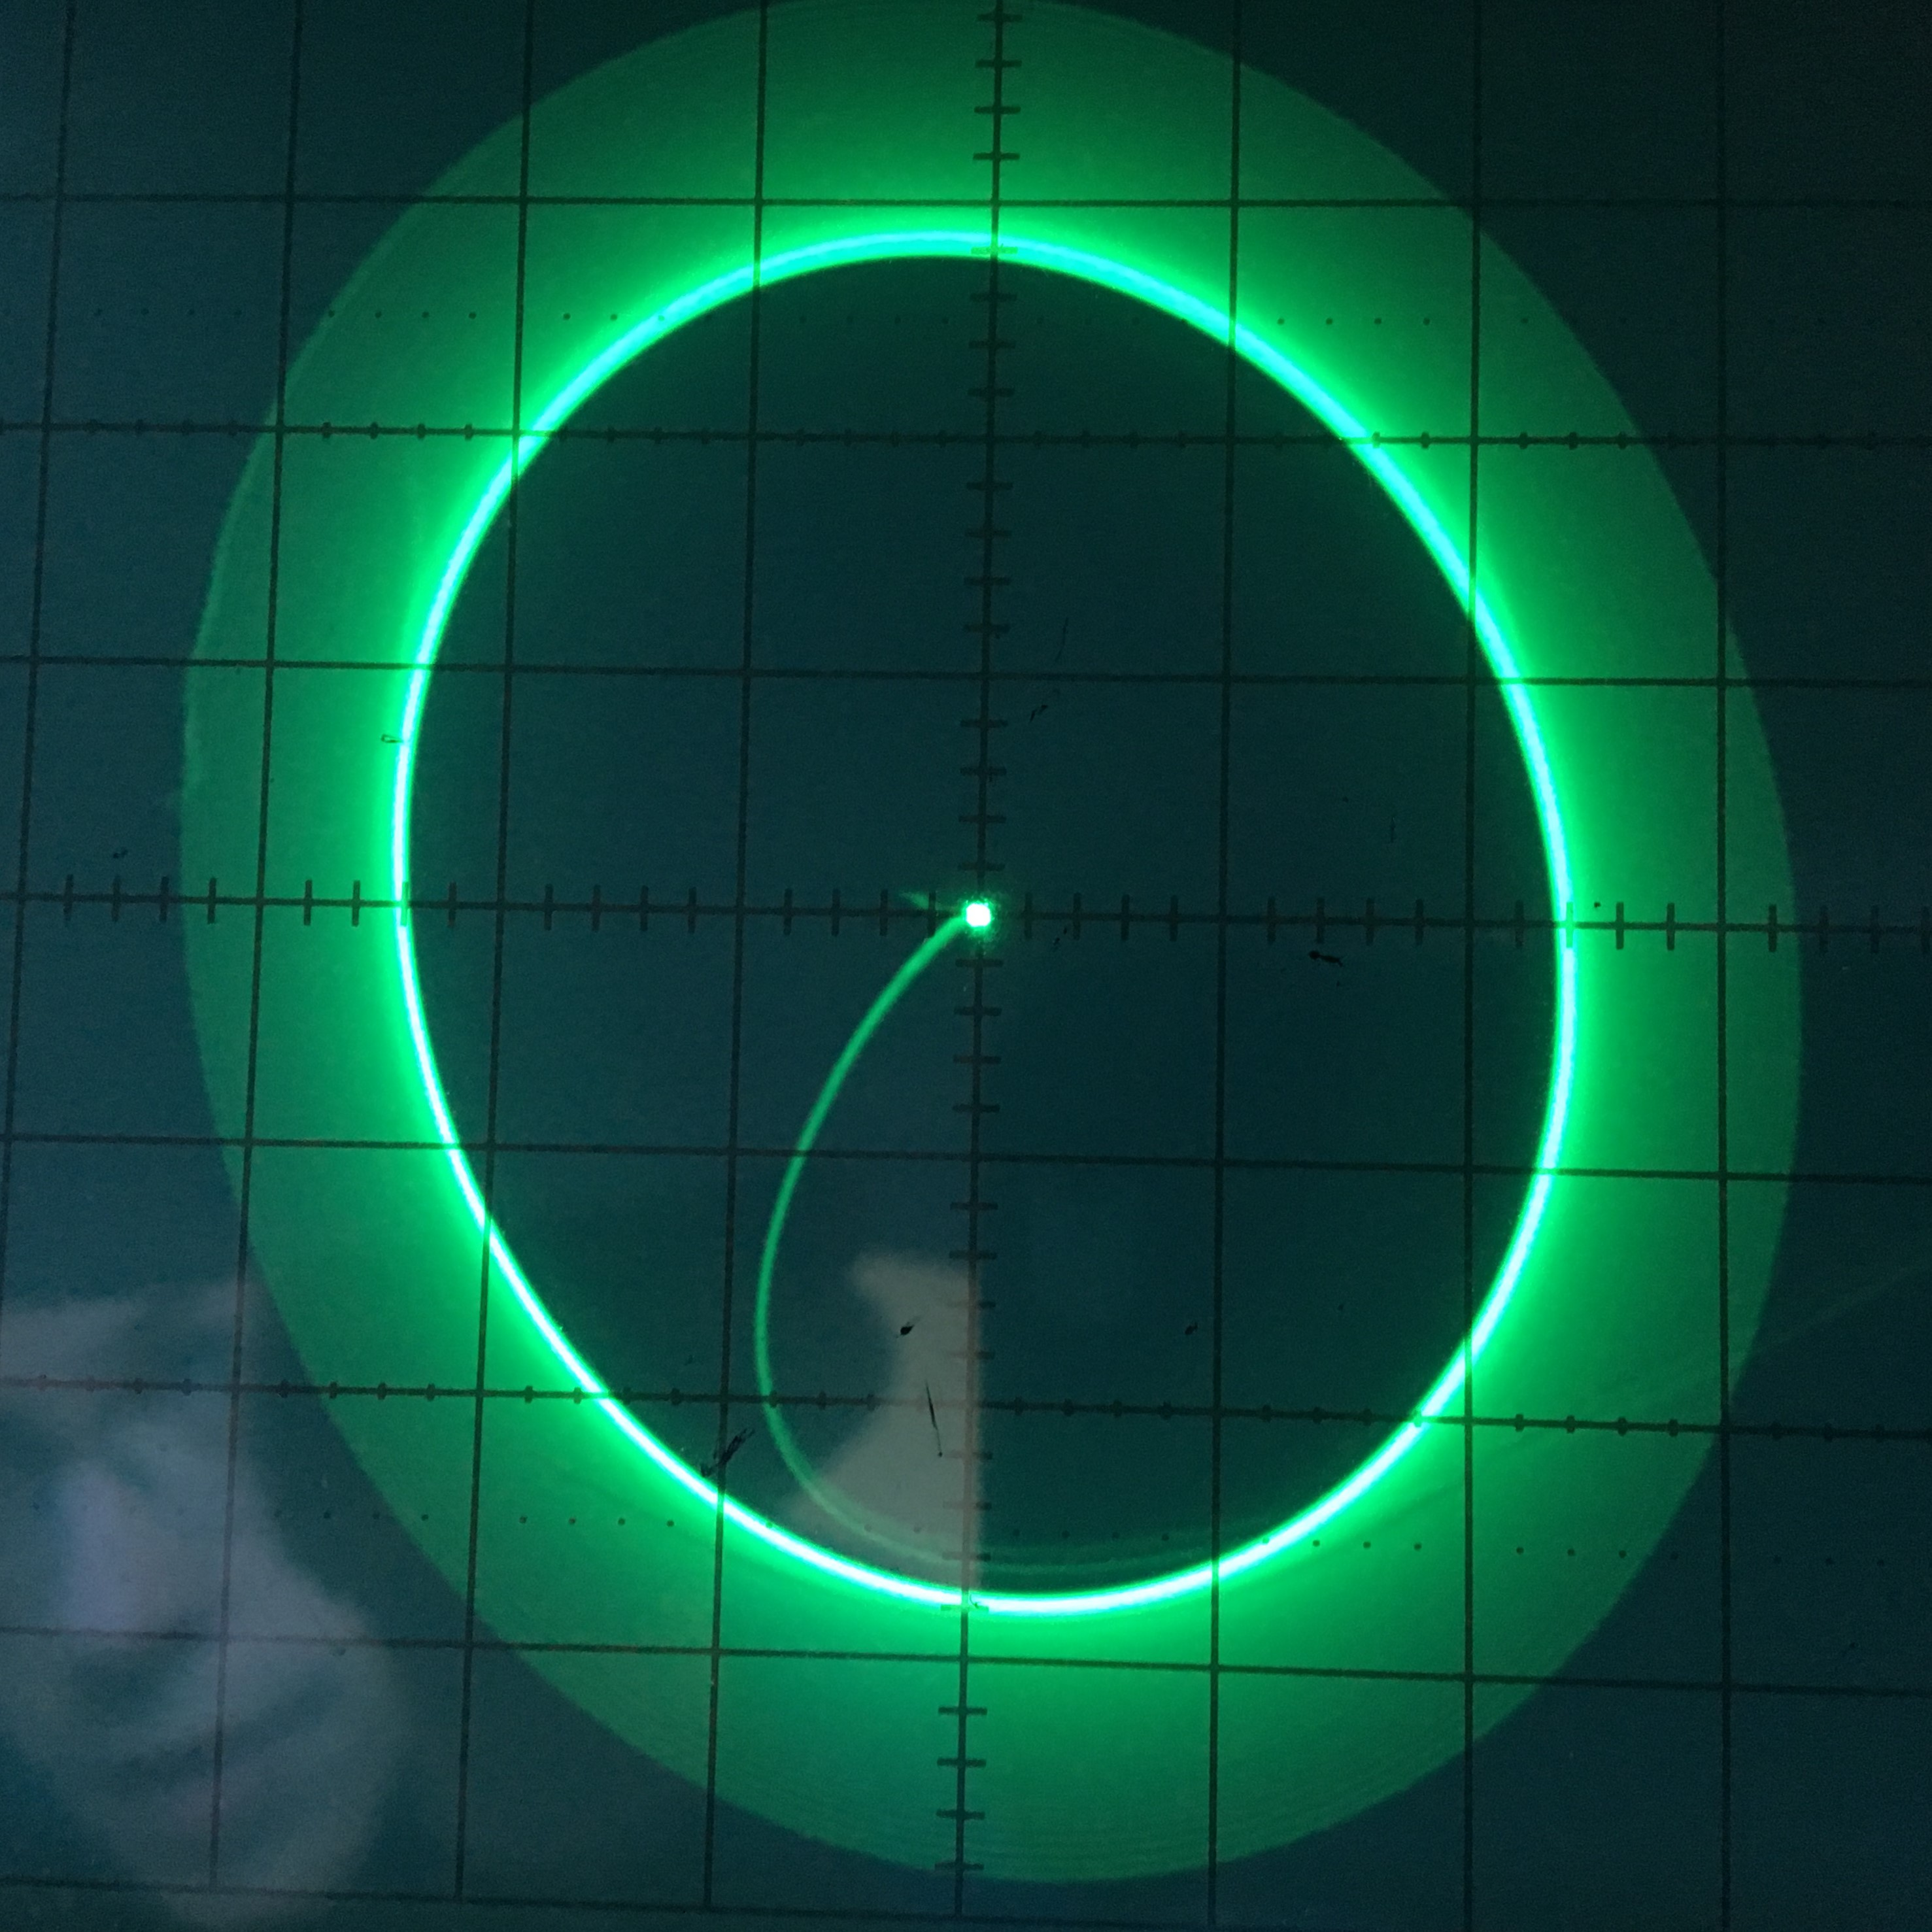
\includegraphics[width=\linewidth]{photo/task1b(rightL).jpg}
	\end{minipage}
	\caption{Правее точки бифрукации}
	\label{fig4}
\end{figure}
По фазовым траекториям видно, что устойчивый режим наблюдается на некотором значении, так как мы находимся правее точки бифрукации.
\subsubsection{Квазипериодические затухания}
Уменьшая обратную связь, получили квазипериодический затухающий процесс.
\begin{figure}[h]
	\centering
	\begin{minipage}{0.32\linewidth}
	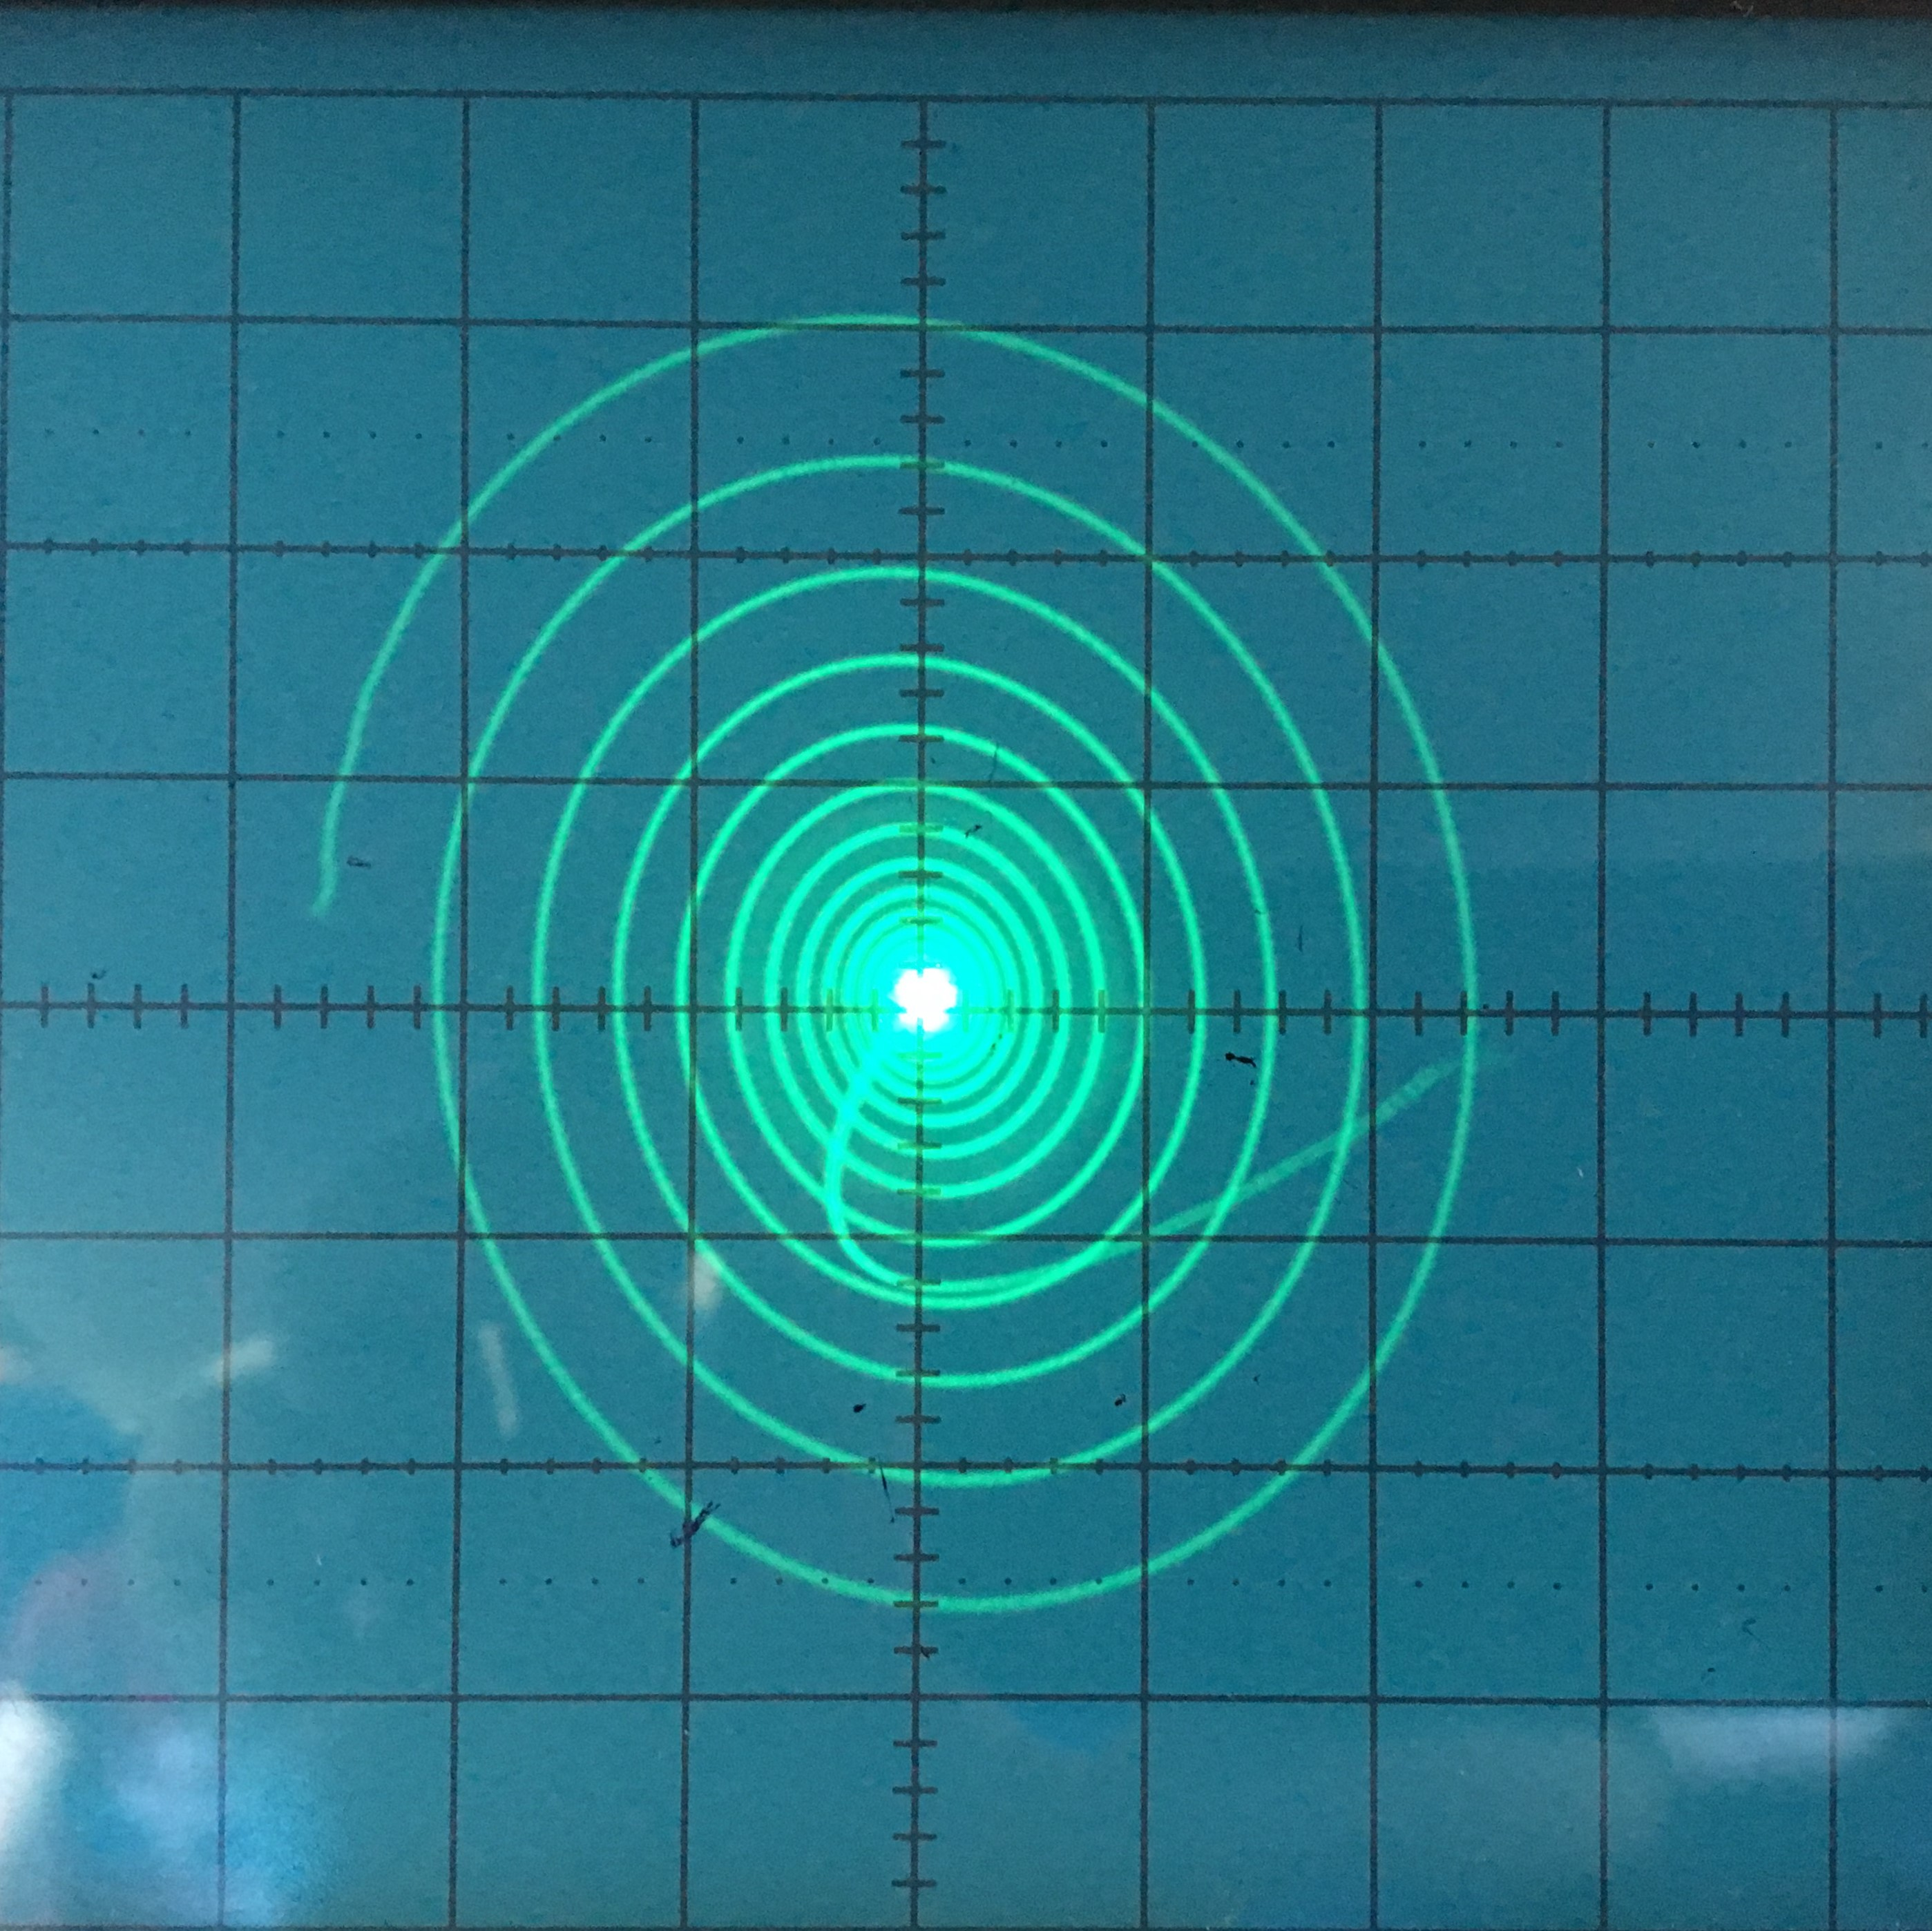
\includegraphics[width=\linewidth]{photo/task1c1.jpg}
	\end{minipage}
	\begin{minipage}{0.32\linewidth}
	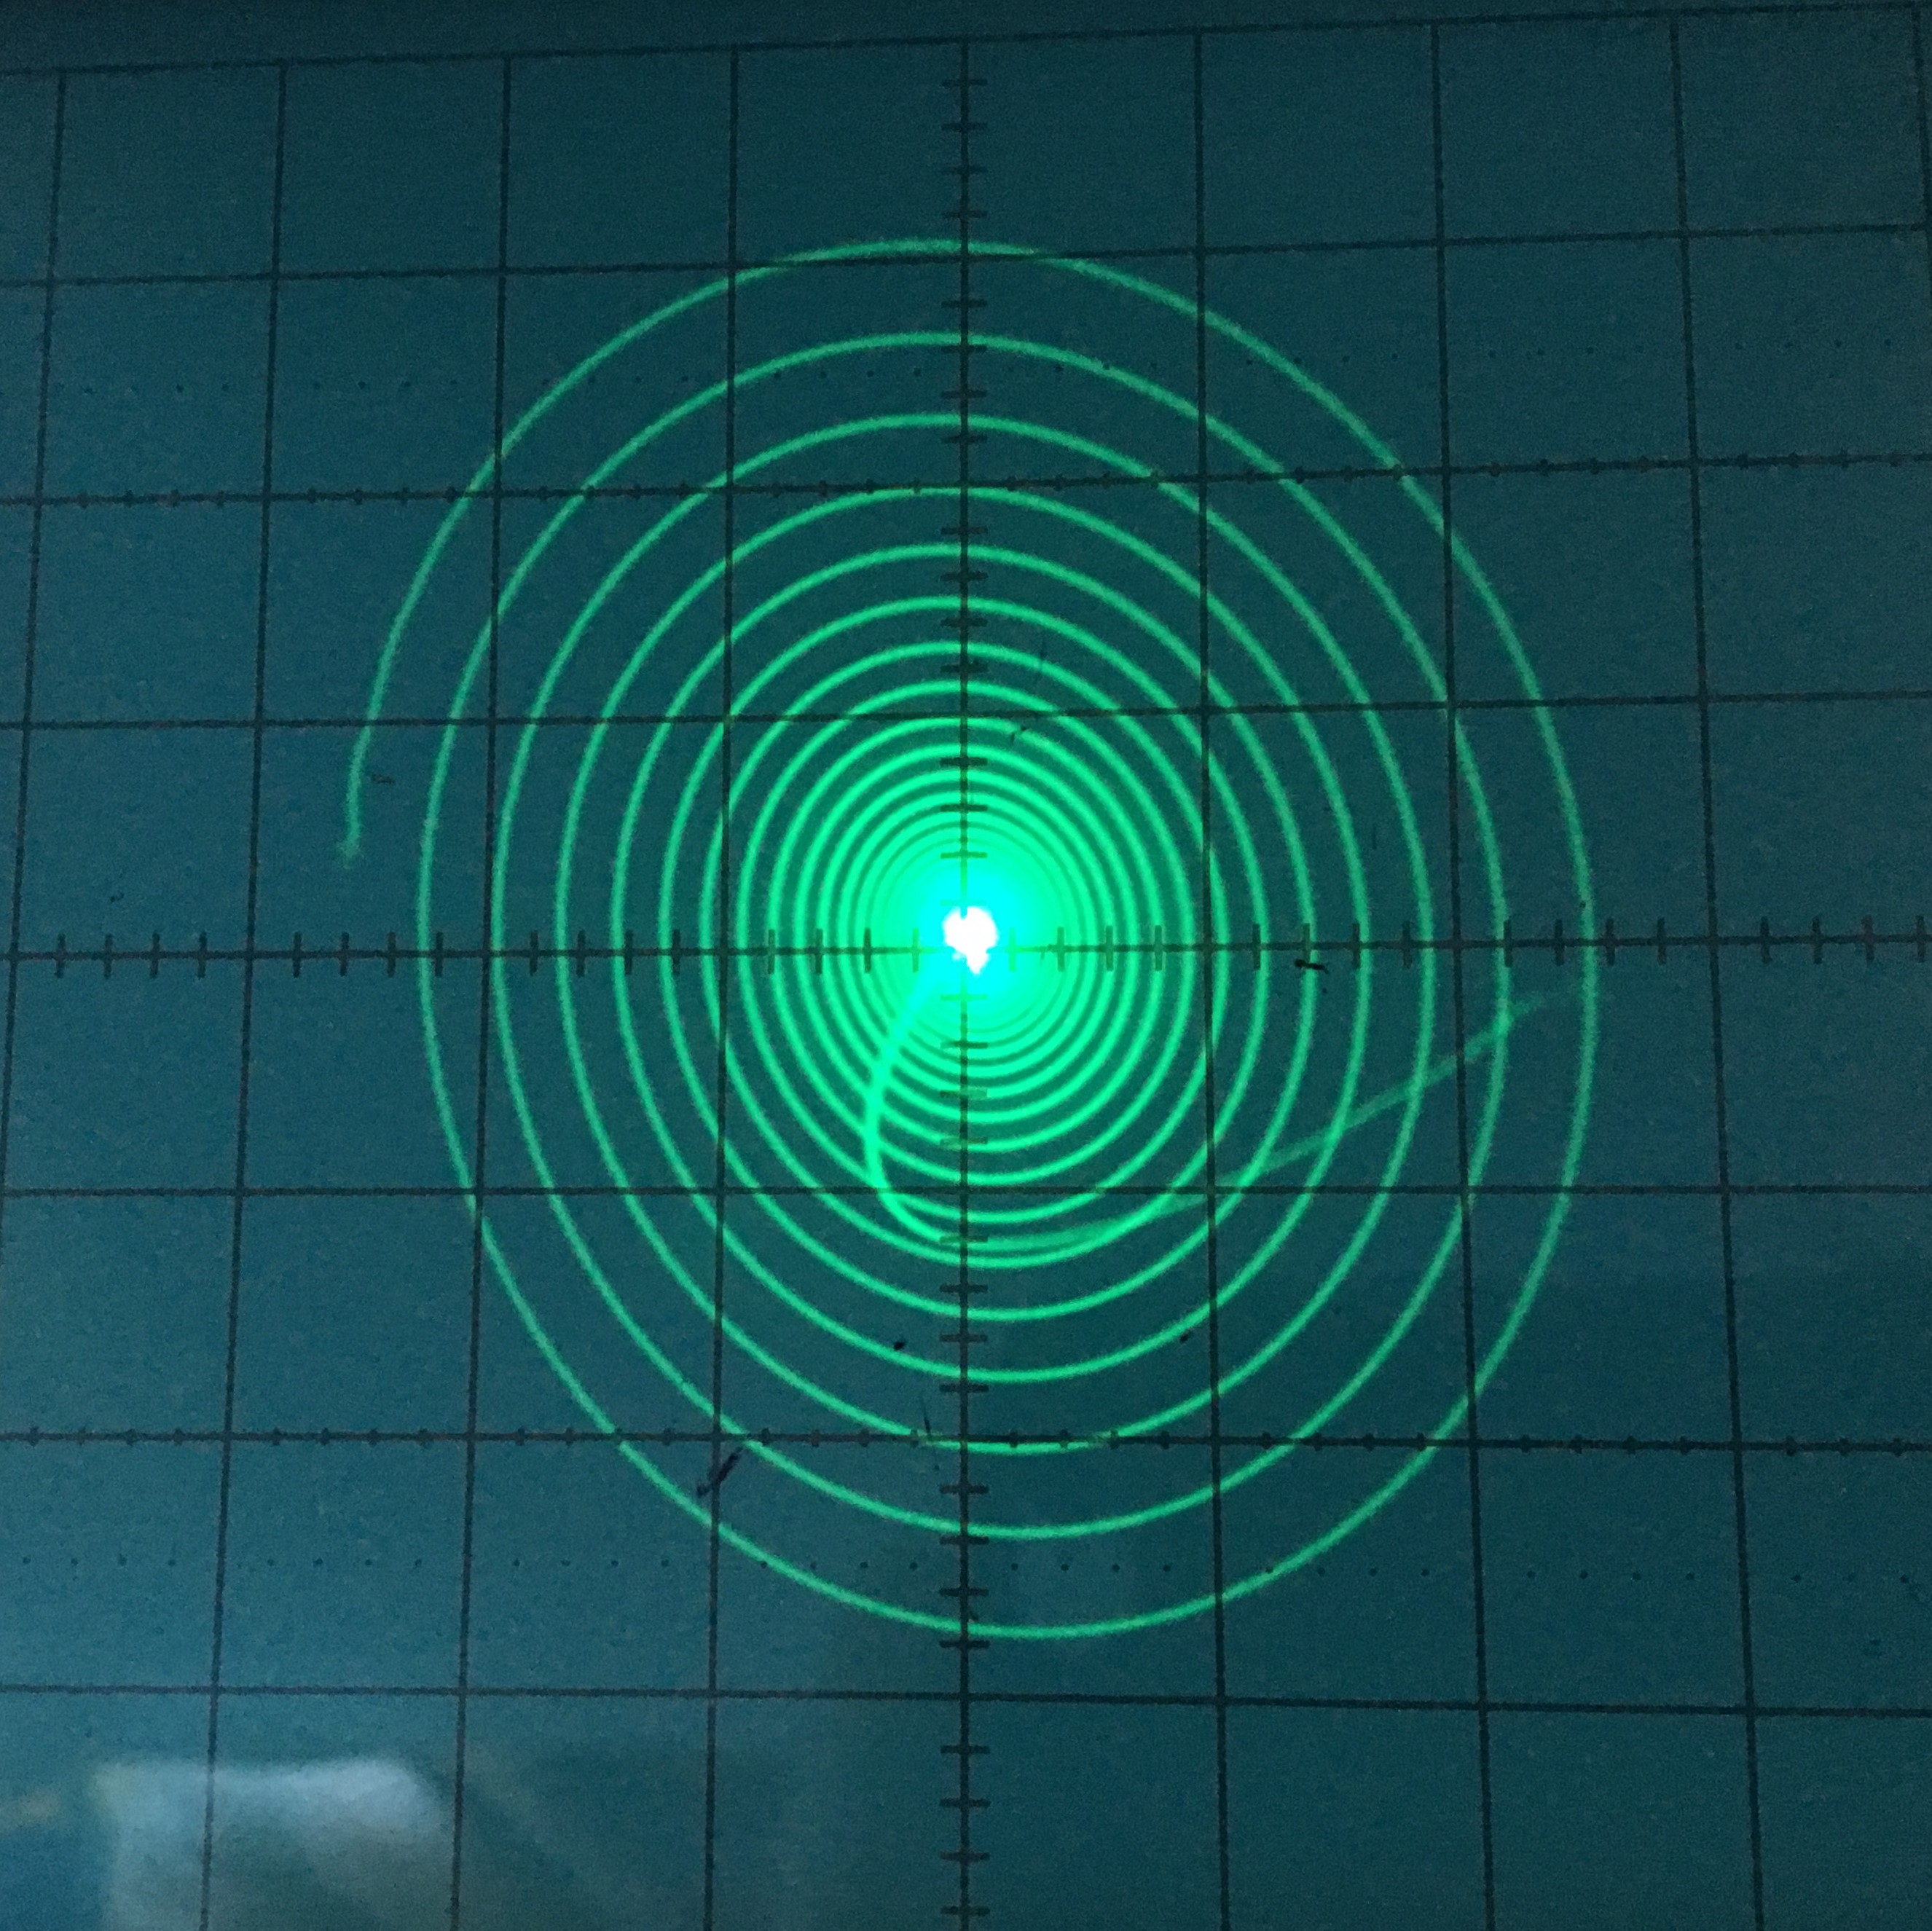
\includegraphics[width=\linewidth]{photo/task1c5.jpg}
	\end{minipage}
	\begin{minipage}{0.32\linewidth}
	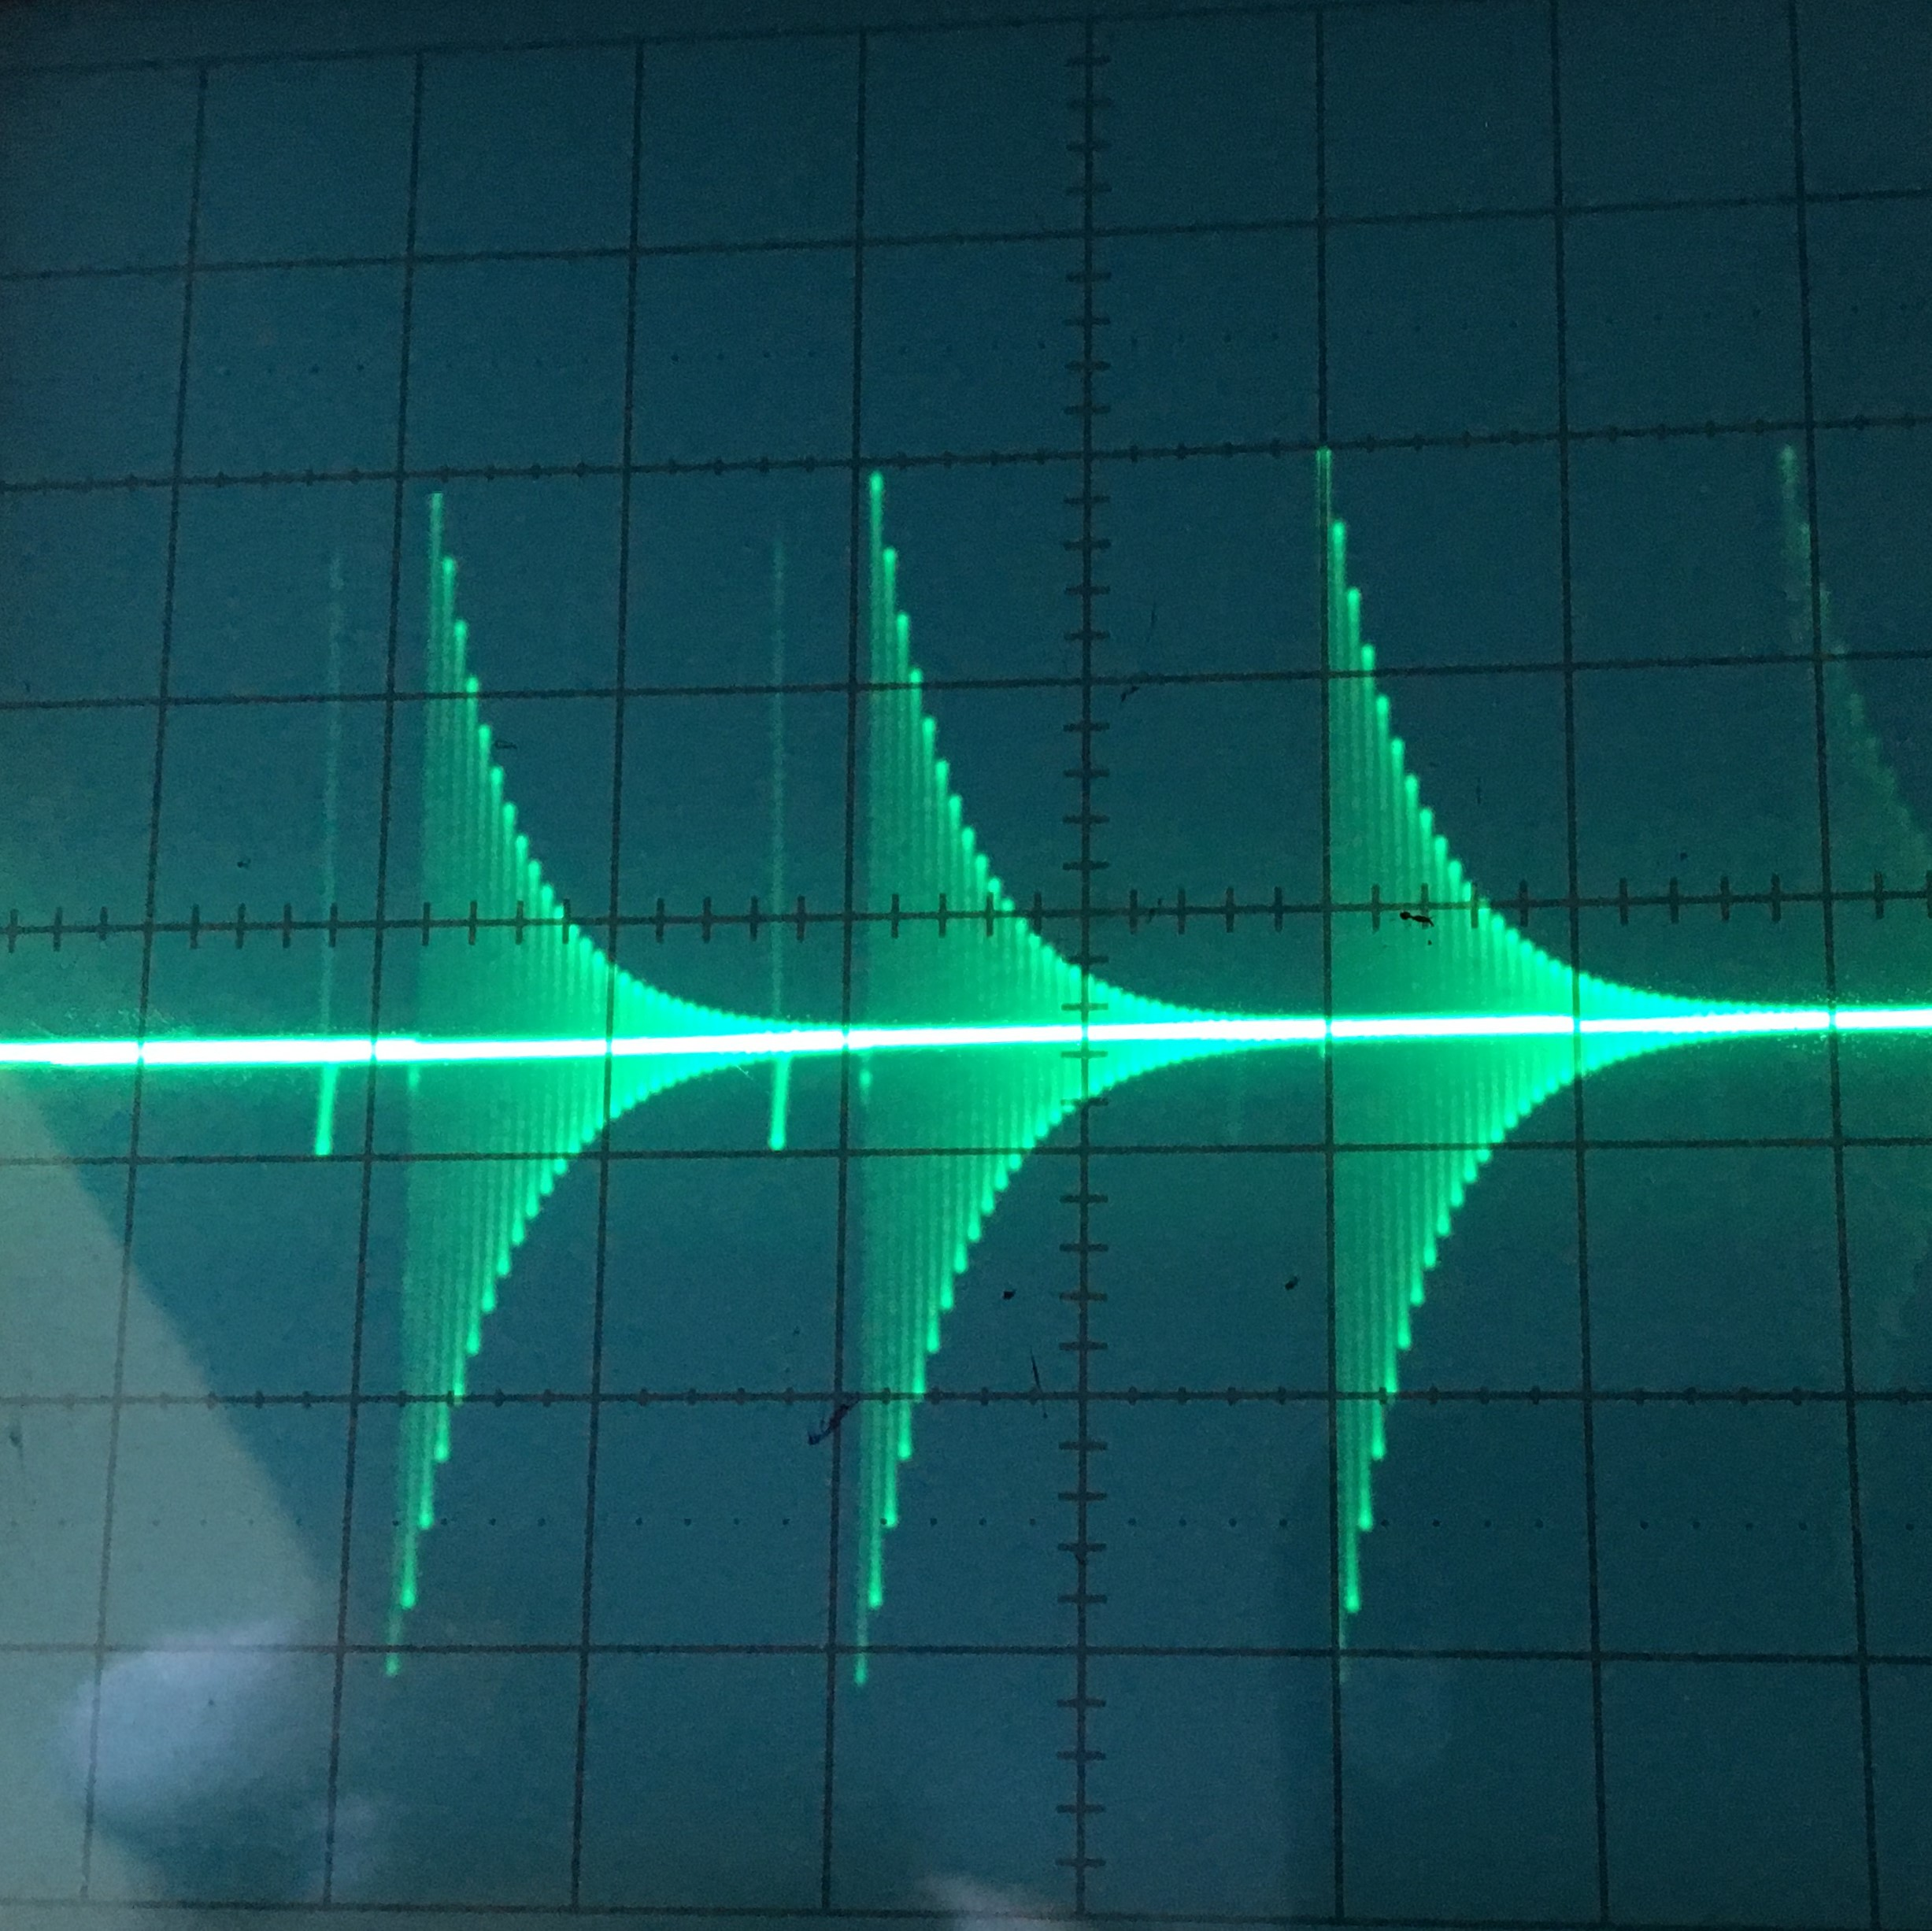
\includegraphics[width=\linewidth]{photo/task1c(oscill)1.jpg}
	\end{minipage}
    \caption{Фазовые траектории и осцилограмма затухающего процесса}
	\label{fig5}
\end{figure}
По полученным данным определили декремент затухания для двух различных $M$.
% Table generated by Excel2LaTeX from sheet 'мягкий режим'
\begin{table}[htbp]
  \centering
  \caption{Декремент затухания}
    \begin{tabular}{|c|c|c|}
    \toprule
    \textnumero    & $M$     & $\delta$ \\
    \midrule
    1     & 5     & 0.154638 \\
    \midrule
    2     & 0     & 0.20232 \\
    \bottomrule
    \end{tabular}
  \label{tab1}
\end{table}
\subsubsection{Апериодический процесс}
Увеличивая потери в колебательном контуре,старались получить апериодический процесс при различных начальных условиях.
\begin{figure}[h]
	\centering
	\begin{minipage}{0.32\linewidth}
	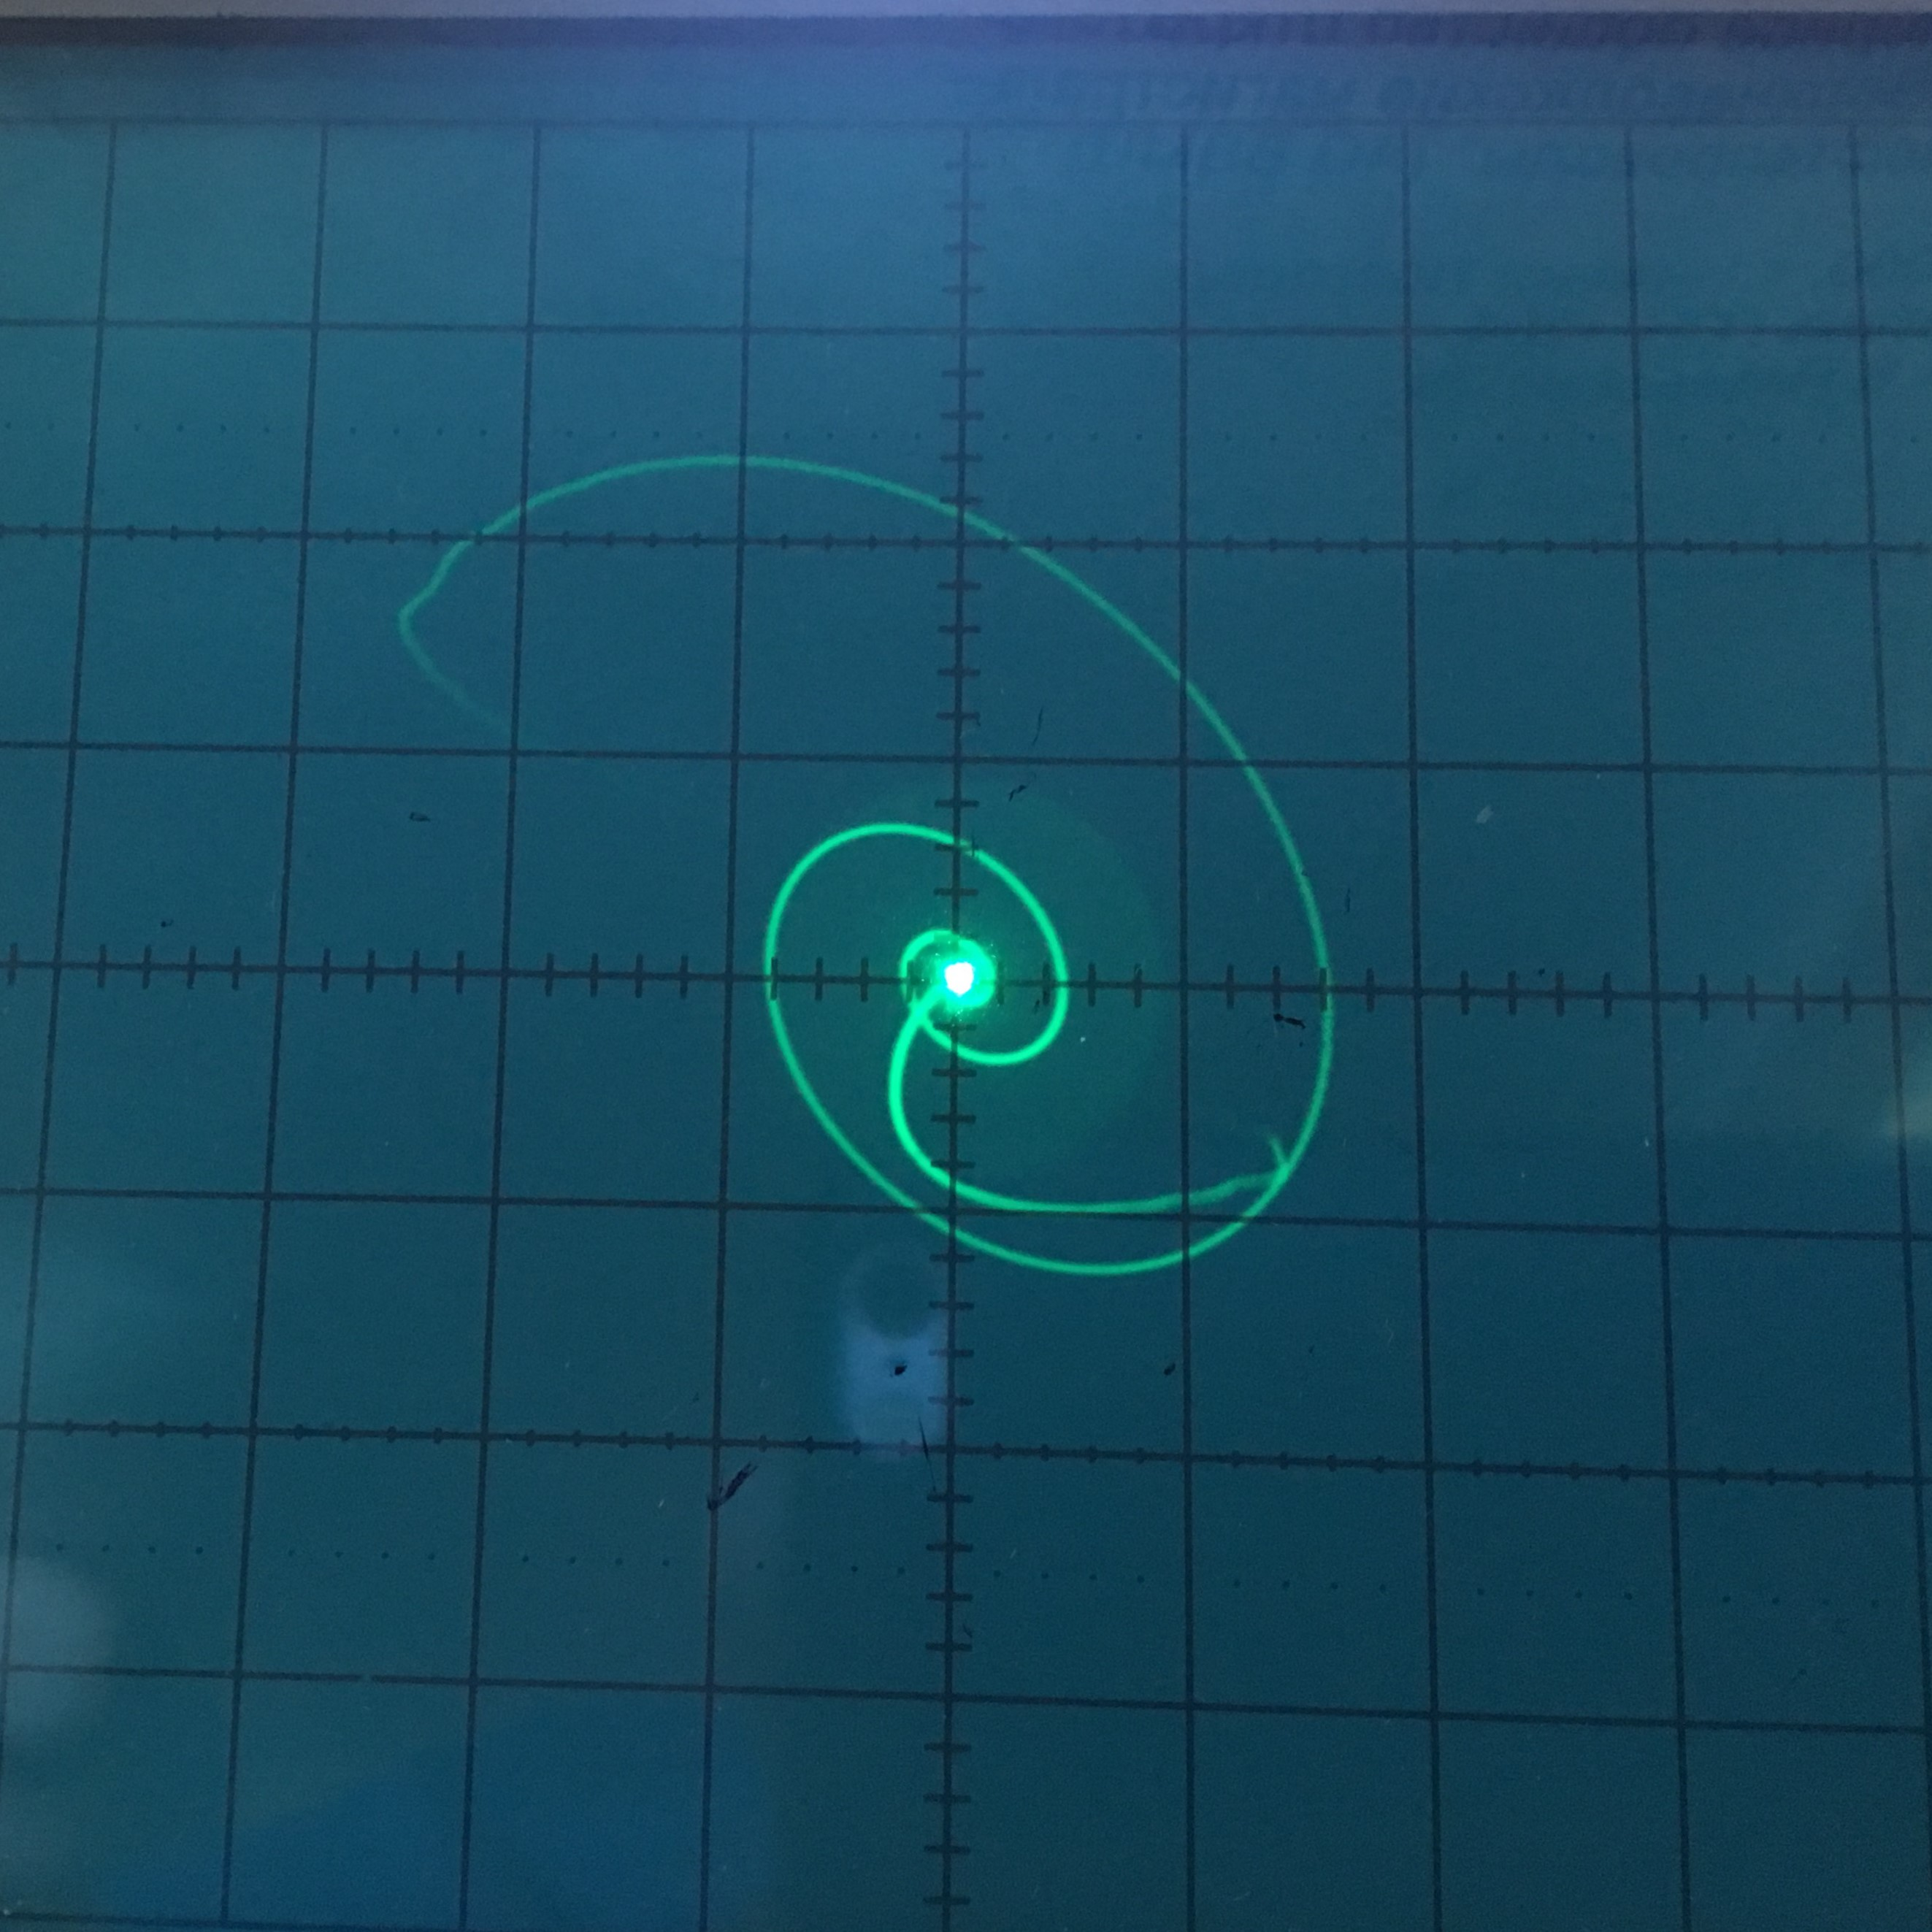
\includegraphics[width=\linewidth]{photo/task1d1.jpg}
	\end{minipage}
	\caption{Фазовый портрет при максимальных потерях в контуре}
	\label{fig6}
\end{figure}
Из фазового портрета видно, что апериодический процесс не наблюдался ни при каких начальных условиях.
\subsection{Жесткий режим генератора}
\subsubsection{Бифрукационная диаграмма}
Сняли бифуркационную диаграмму, выражающую зависимость амплитуды автоколебаний от величины взаимоиндукции $M$.
\begin{figure}[h]
	\centering
	\vspace{-10pt}
	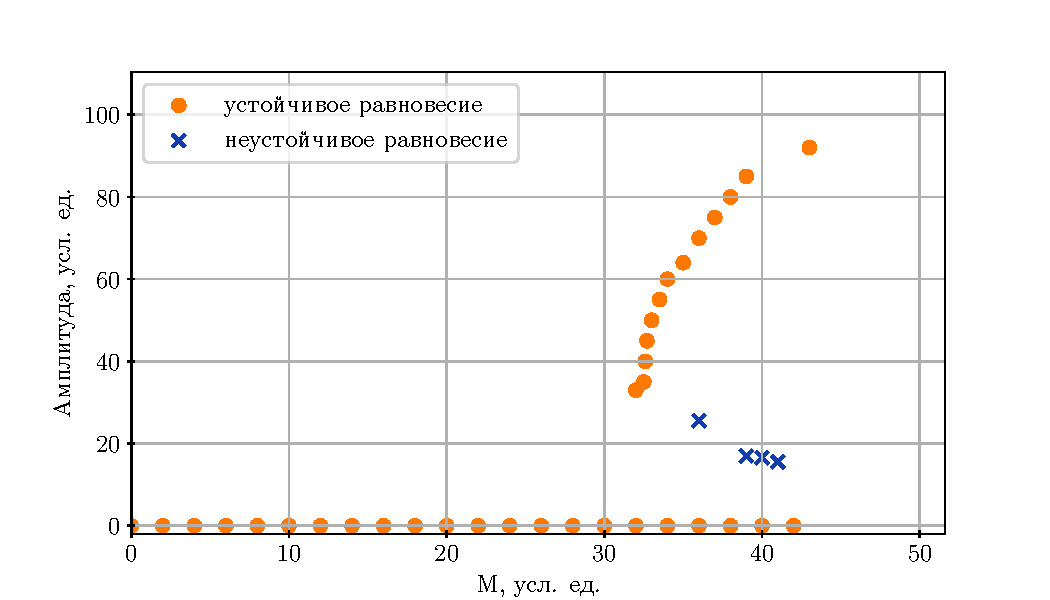
\includegraphics[]{plots/harddiagram.pdf}
	\caption{бифрукационная диаграмма для жесткого режима}
	\label{fig7}
\end{figure}
По полученной диаграмме $M'=32$ усл. ед., $M''=43$ усл. ед. Здесь также можно наблюдать характерную кривую бифрукационной диаграммы для жесткого типа.
\subsubsection{Определение неустойчивого равновесия}
Неустойчивое равновесие на бифрукационной диаграмме находили следующим образом. Включая прерыватель и, изменяя начальные условия, определили по поведению фазовой траектории на экране осциллографа момент перехода изображающей точки через границу области притяжения устойчивого предельного цикла. Оценку амплитуды неустойчивого цикла проводили по фазовой траектории, нормируя ее на амплитуду устойчивого цикла. Оценку также можно оценить по осцилограмме в режиме развертки.
\begin{figure}[h]
	\centering
	\begin{minipage}{0.32\linewidth}
	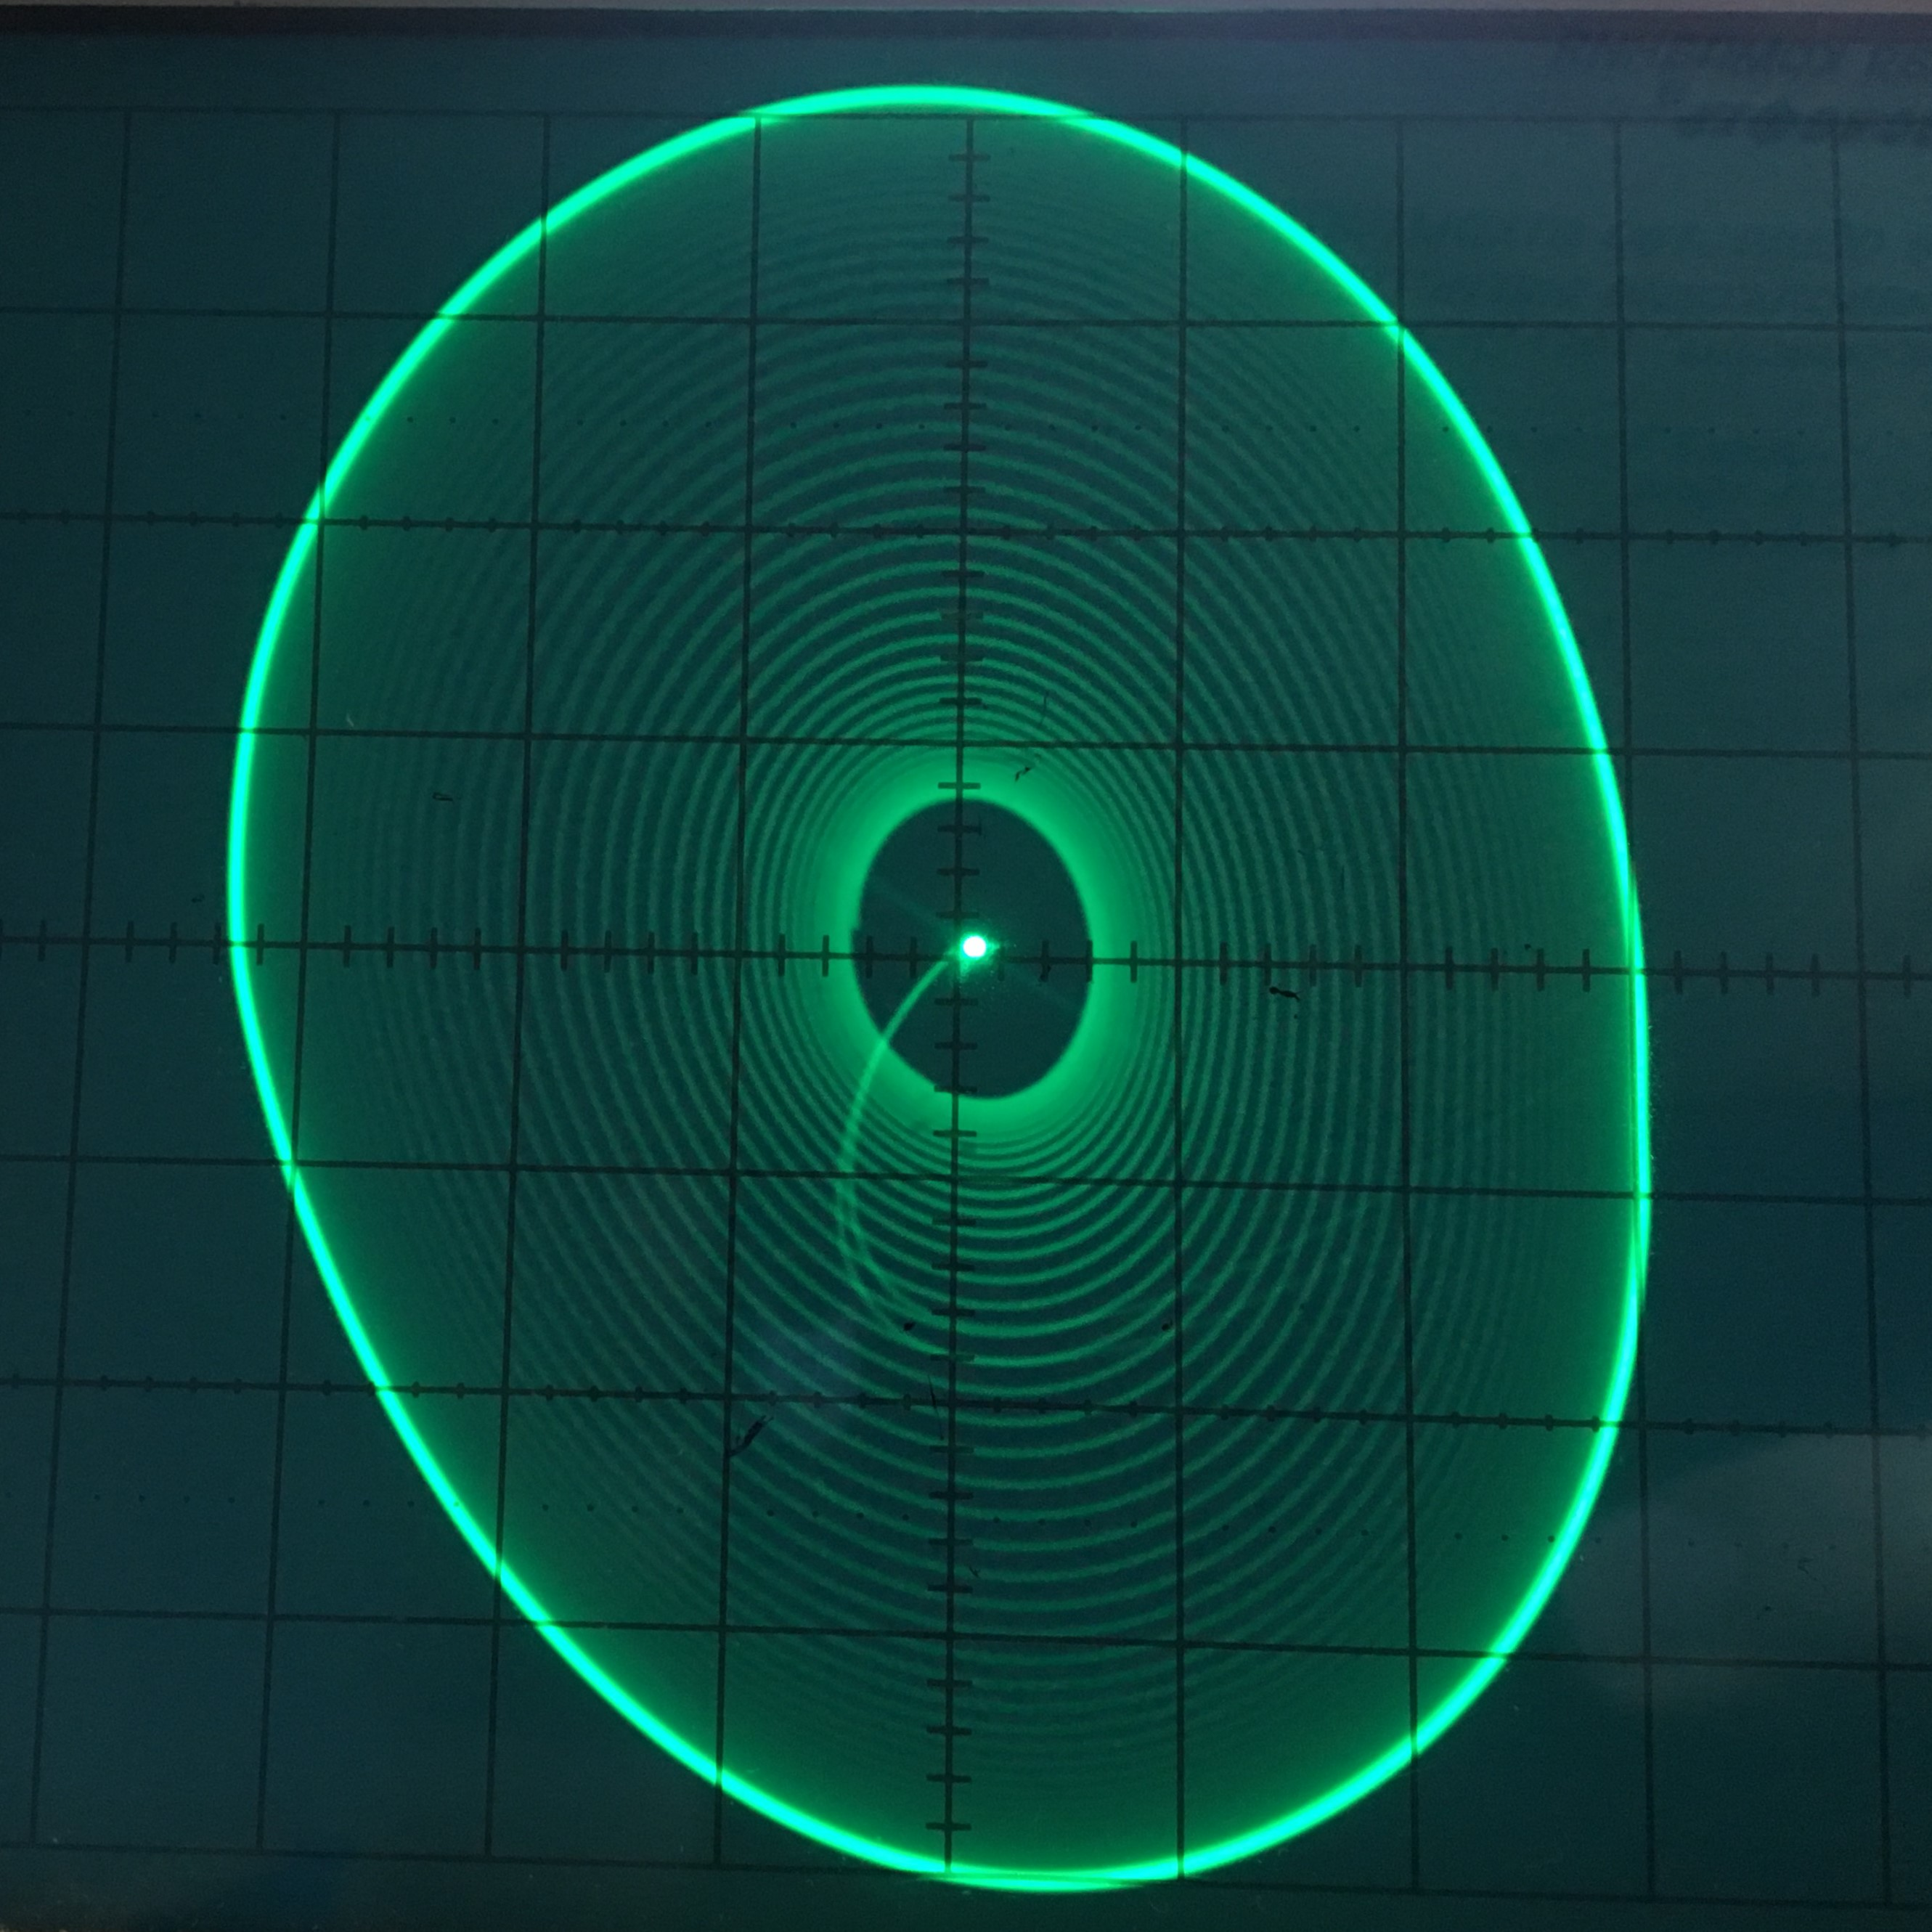
\includegraphics[width=\linewidth]{photo/task2b2.jpg}
	\end{minipage}
	\begin{minipage}{0.32\linewidth}
	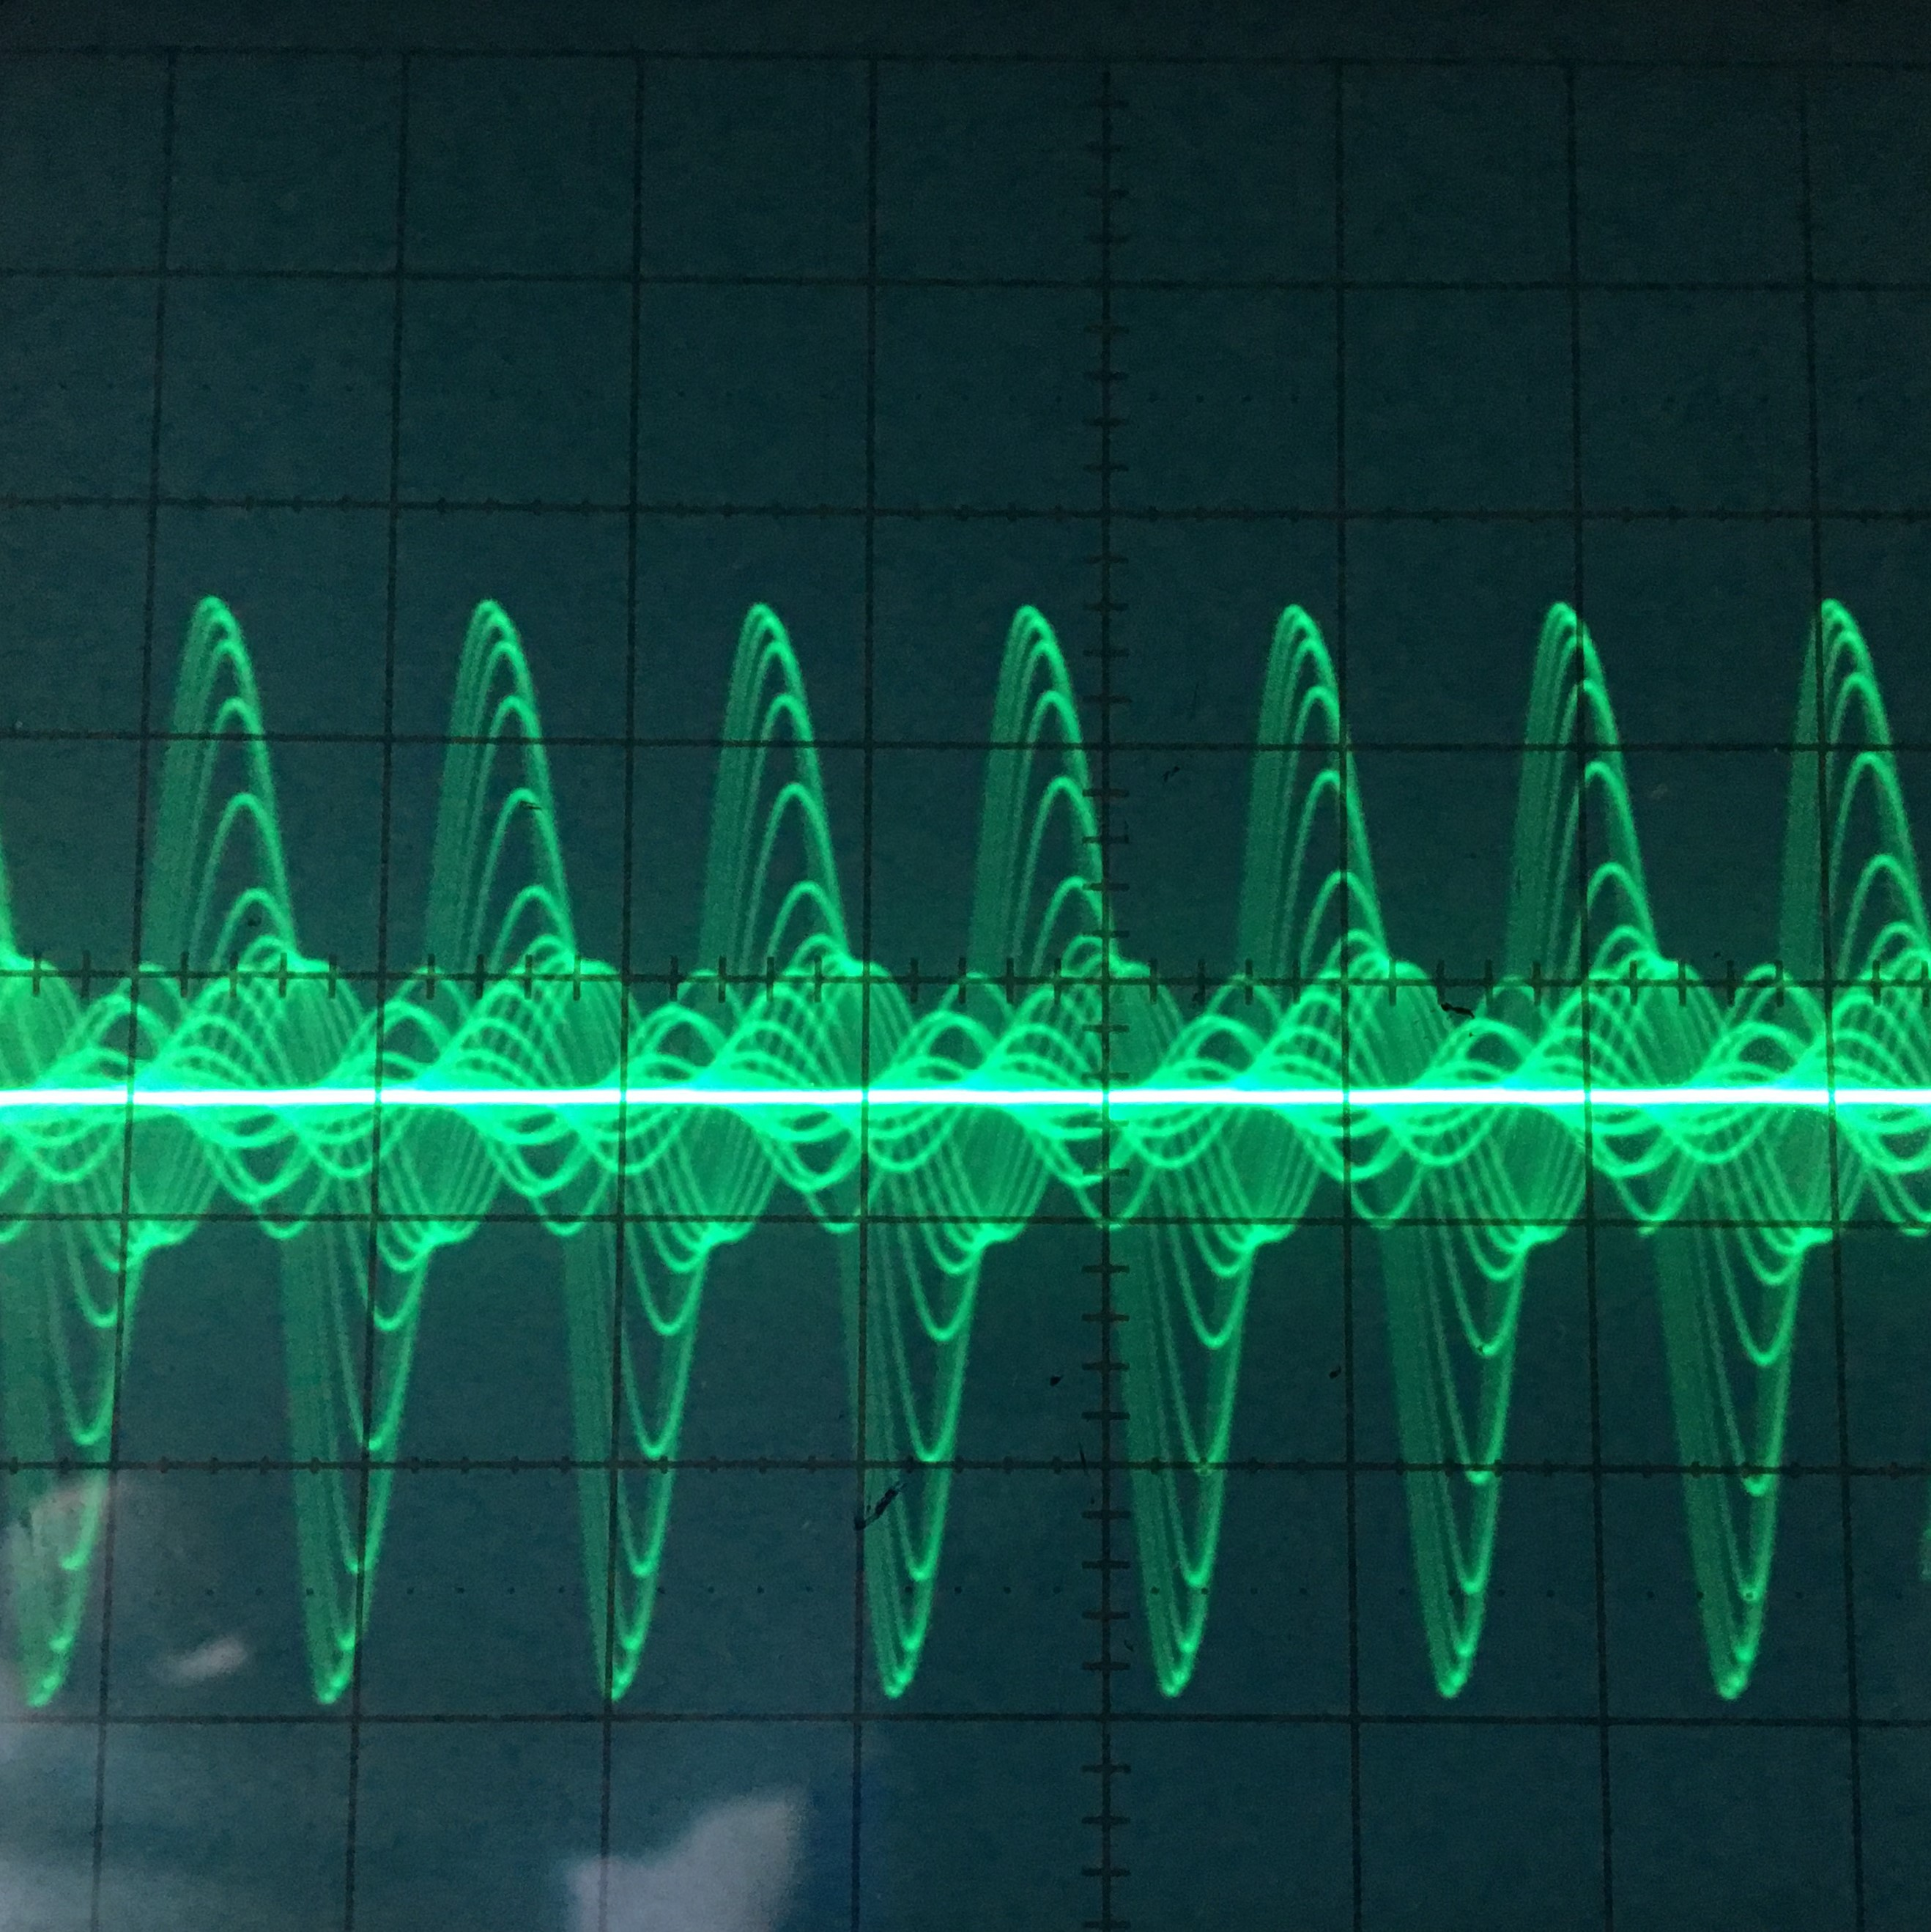
\includegraphics[width=\linewidth]{photo/task2b1(oscill).jpg}
	\end{minipage}
	\caption{Фазовые траектории и осцилограмма неустойчивого предельного цикла}
	\label{fig8}
\end{figure}
\subsubsection{Фазовые траектории}
Получили фазовые траектории при различных начальных условиях для трех значений $M$($M<M',M'<M<M'',M>M''$).
\begin{figure}[h]
	\centering
	\begin{minipage}{0.32\linewidth}
	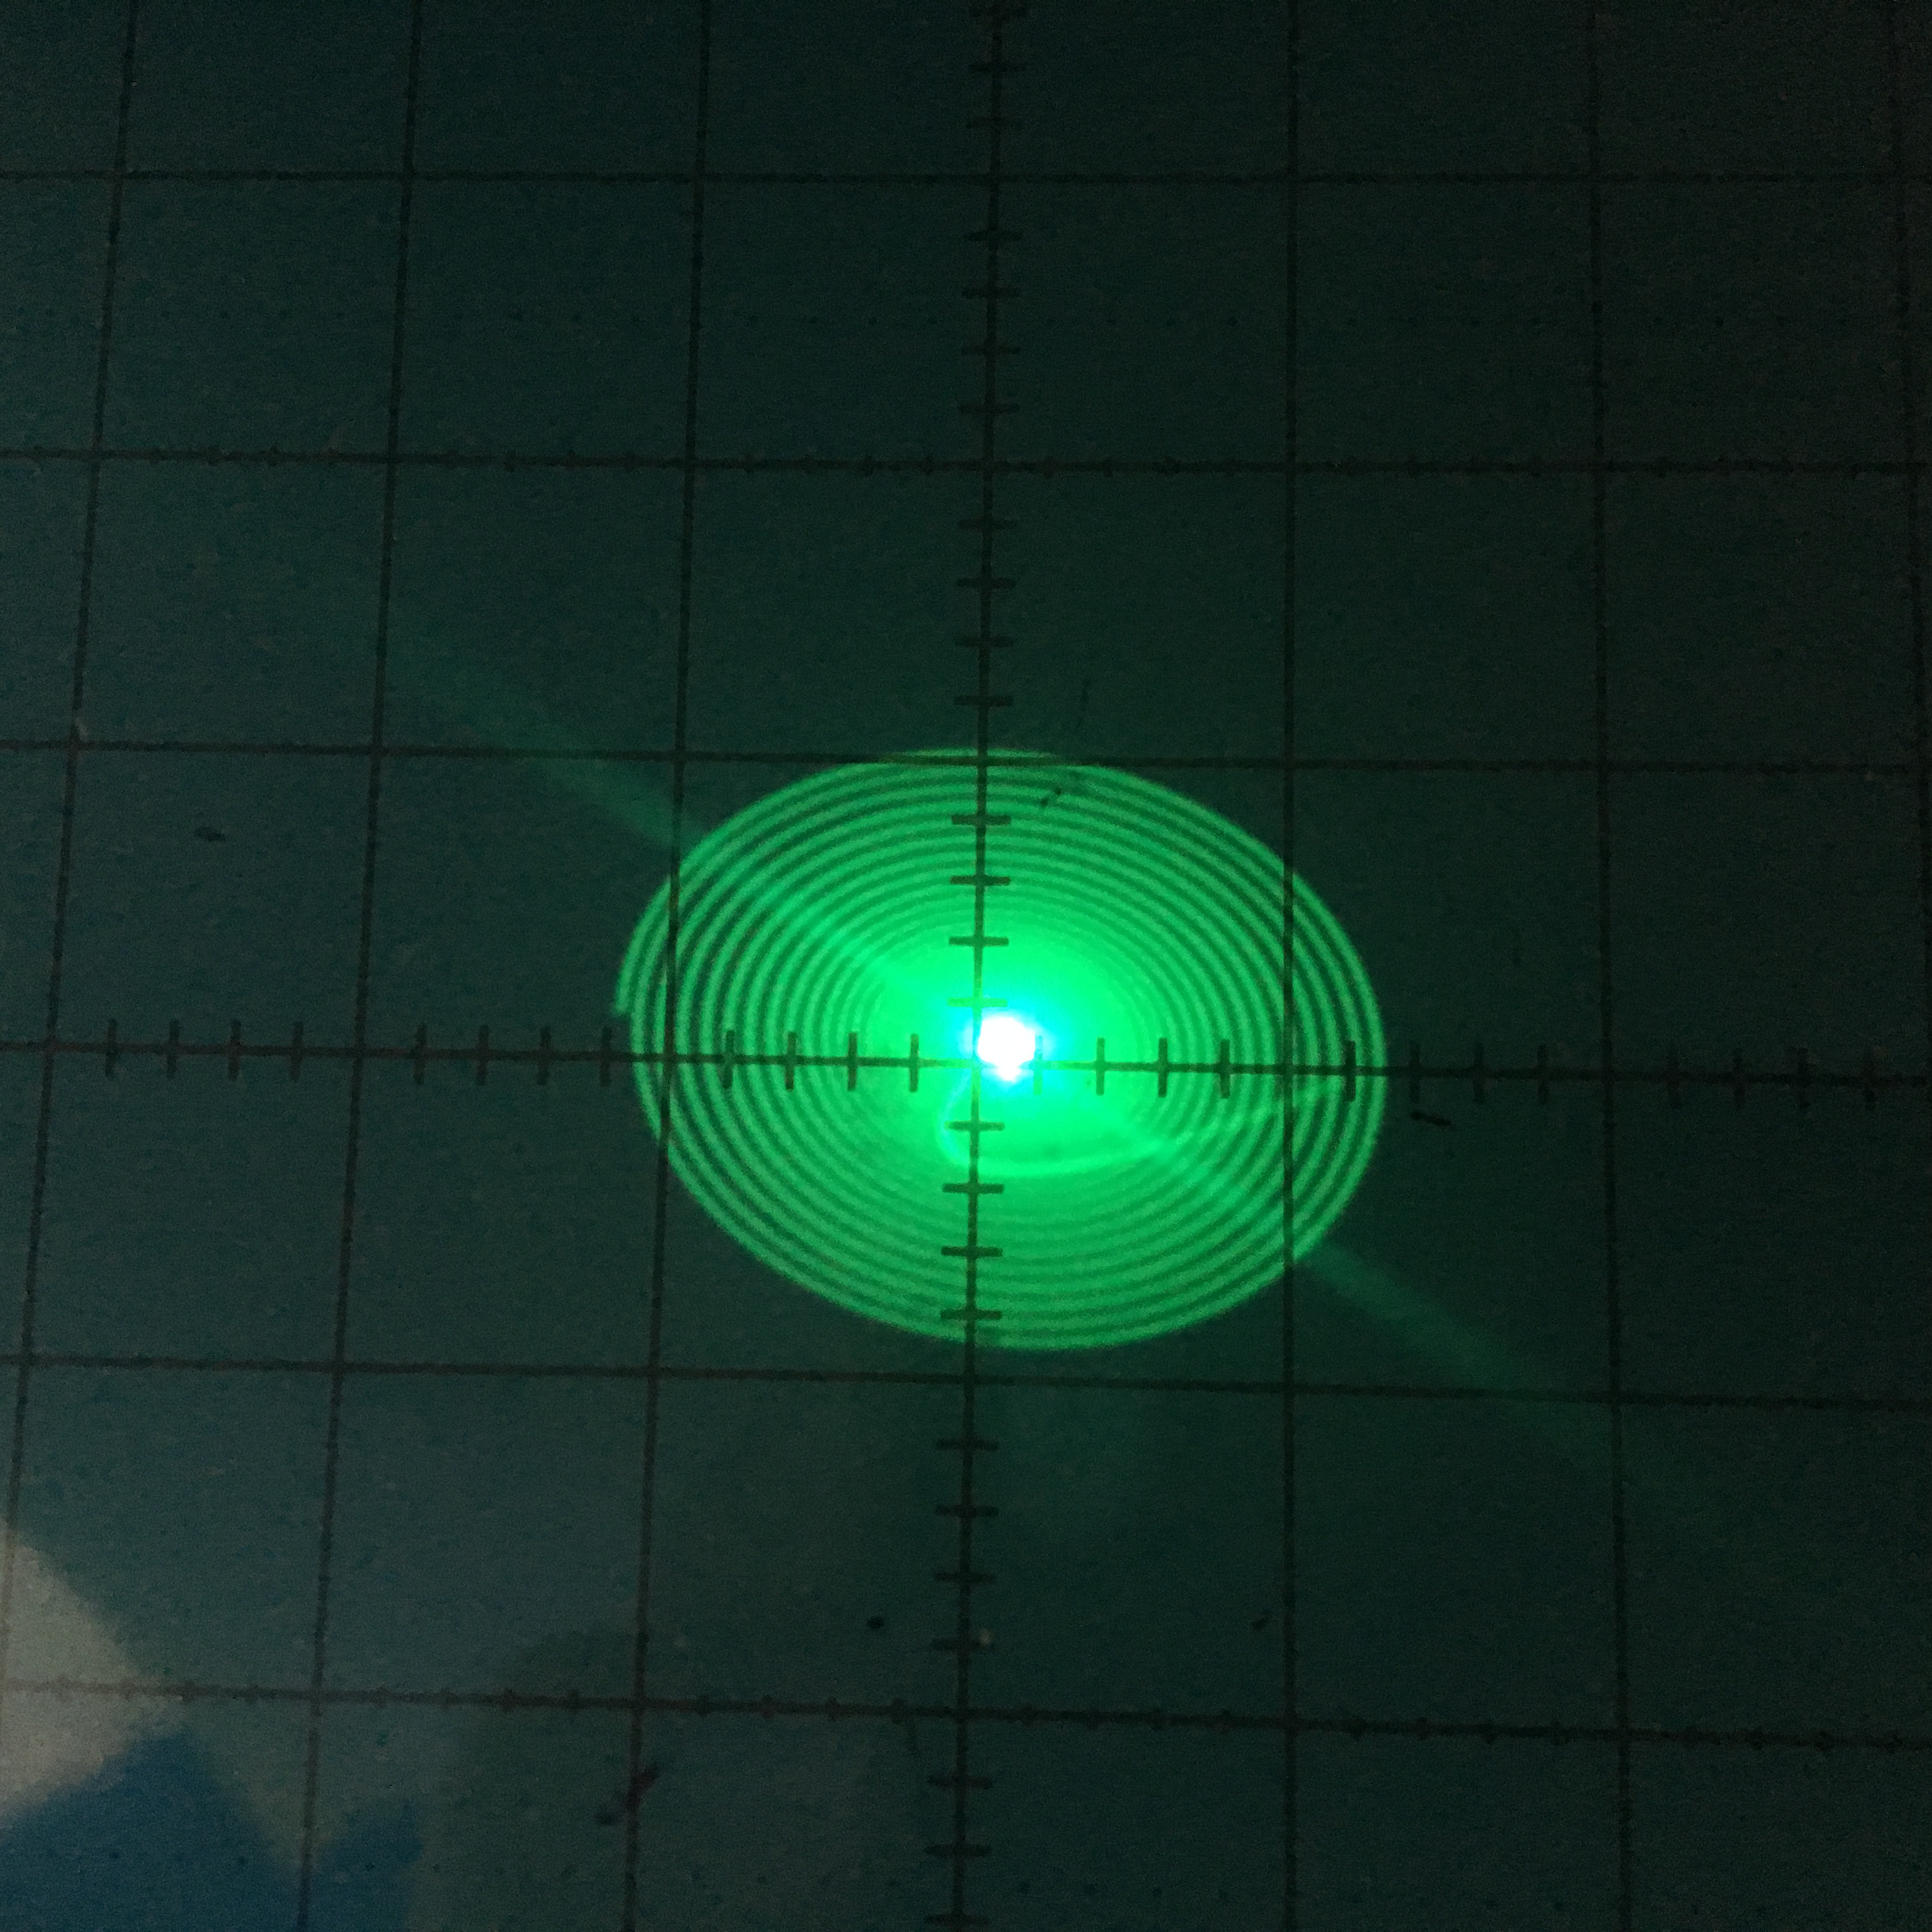
\includegraphics[width=\linewidth]{photo/task2c(lefts).jpg}
	\end{minipage}
	\begin{minipage}{0.32\linewidth}
	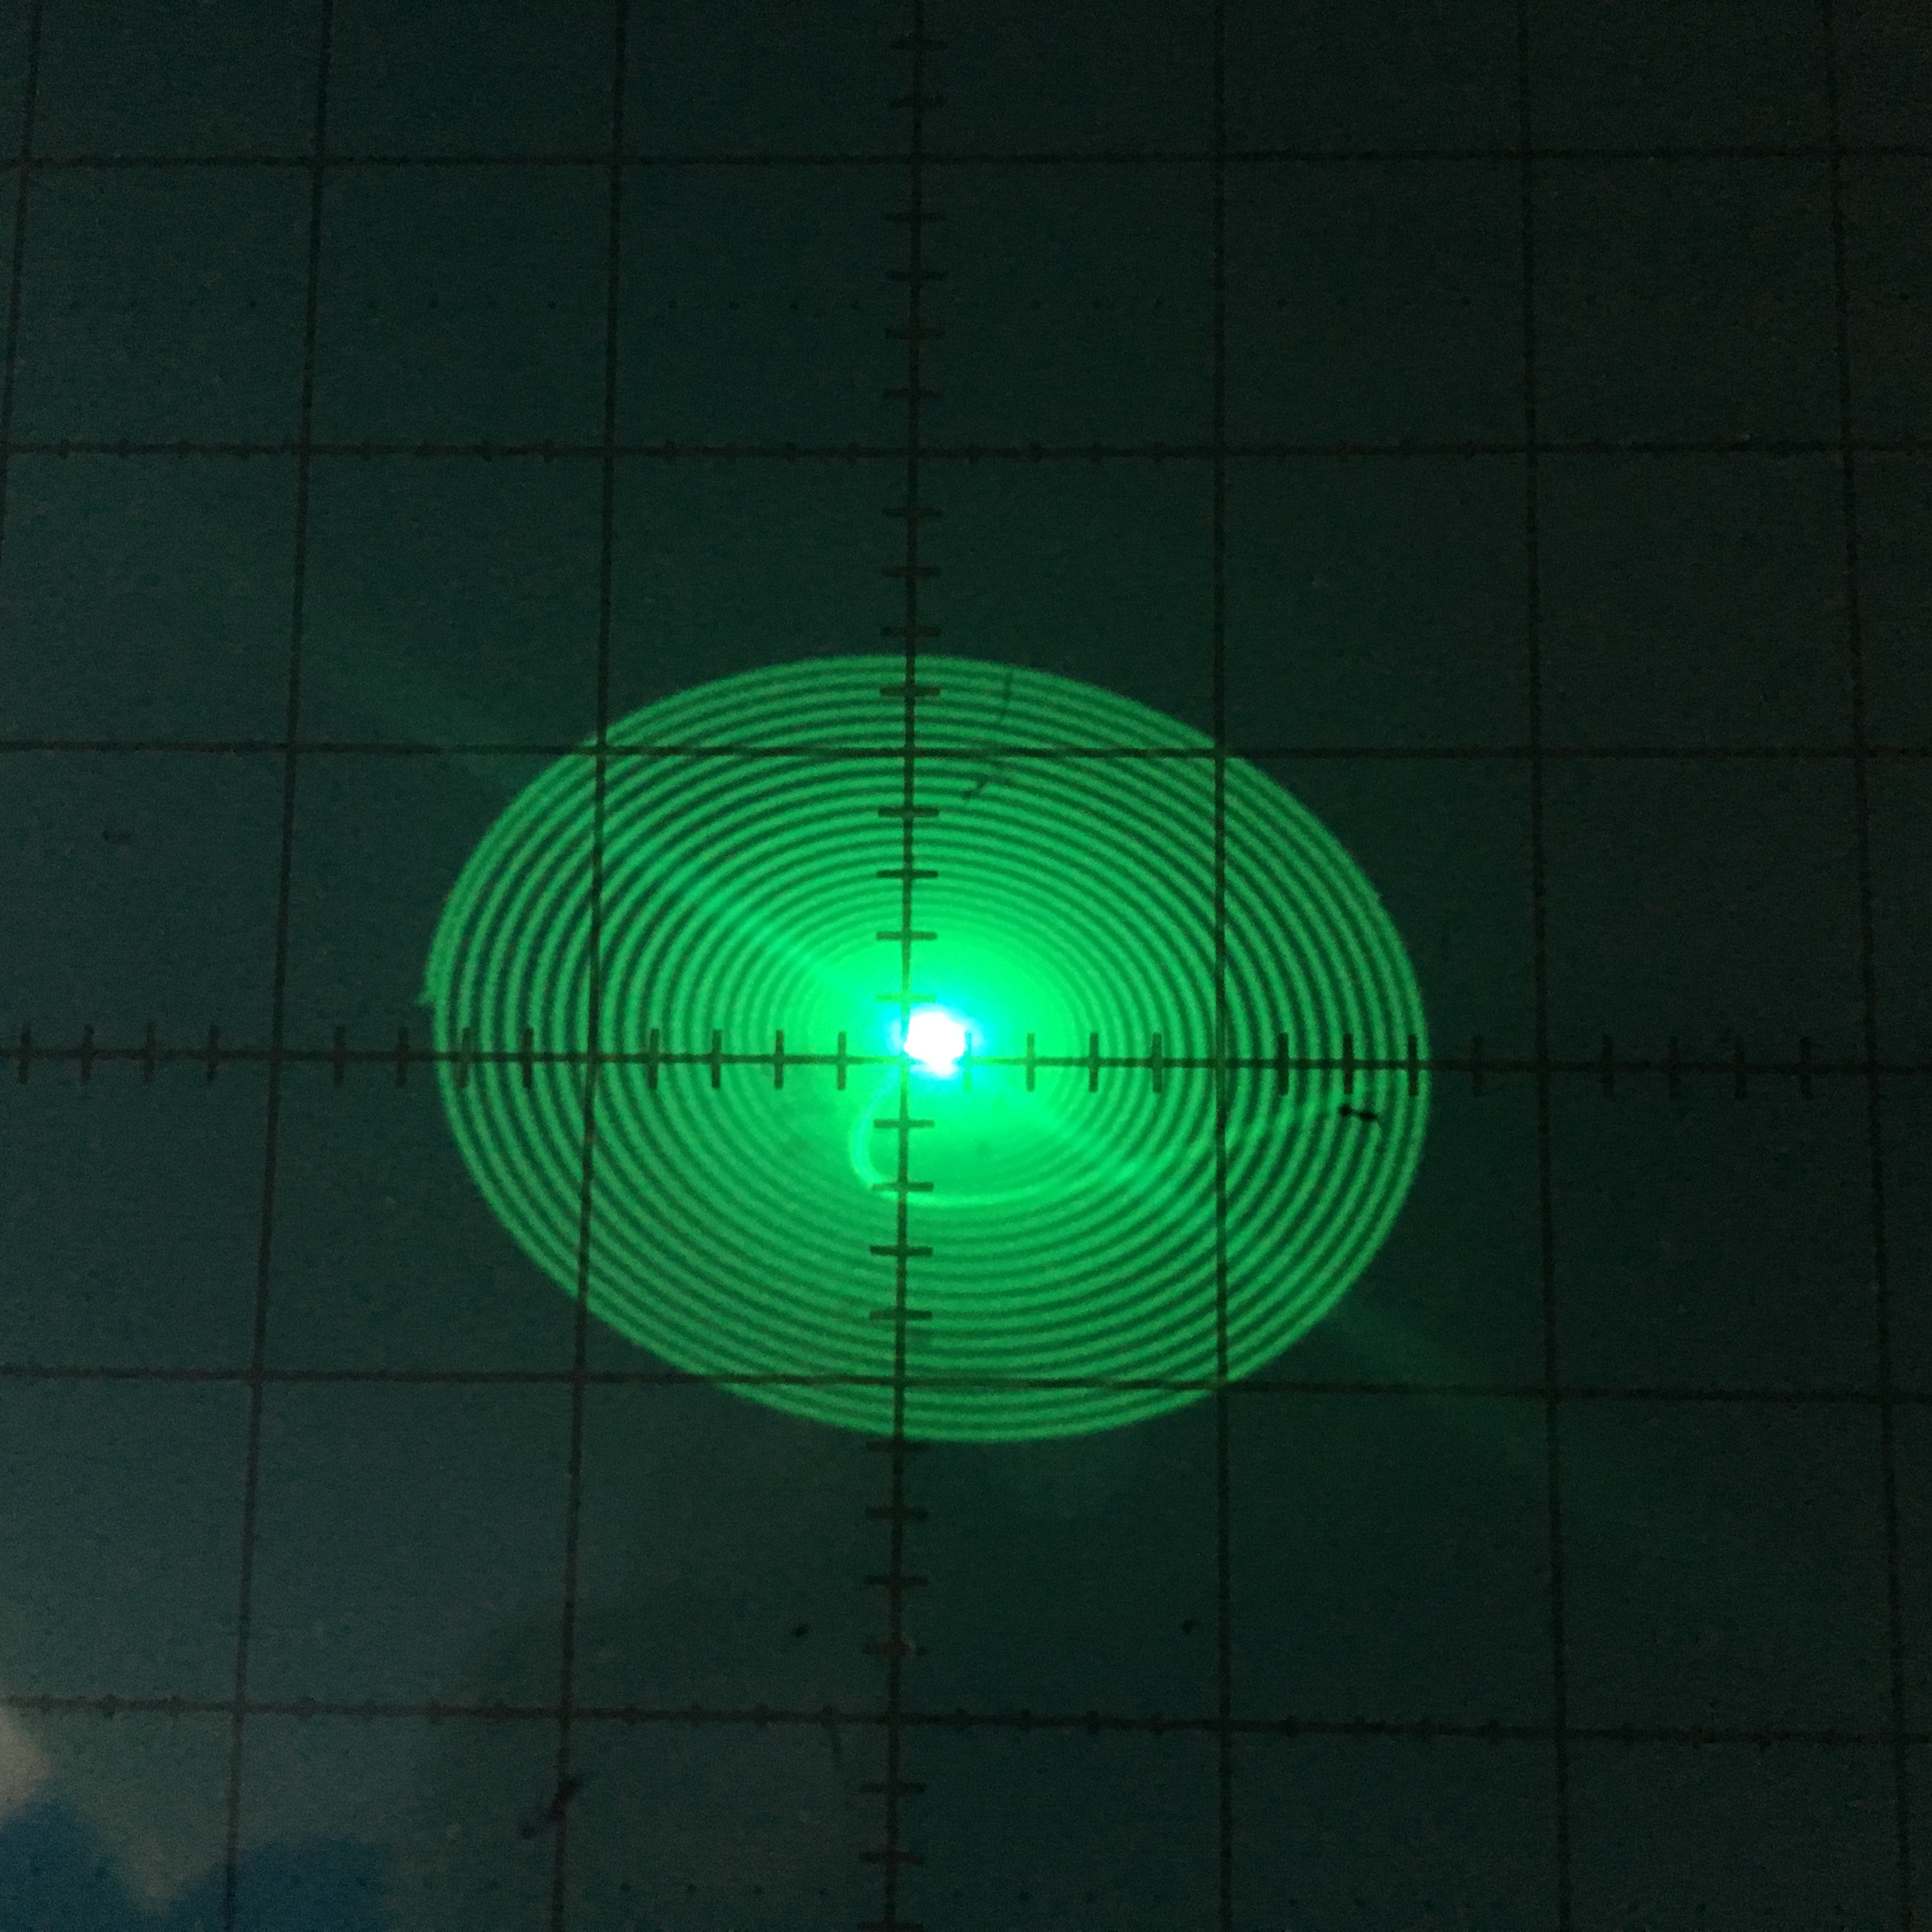
\includegraphics[width=\linewidth]{photo/task2c(leftm).jpg}
	\end{minipage}
	\begin{minipage}{0.32\linewidth}
	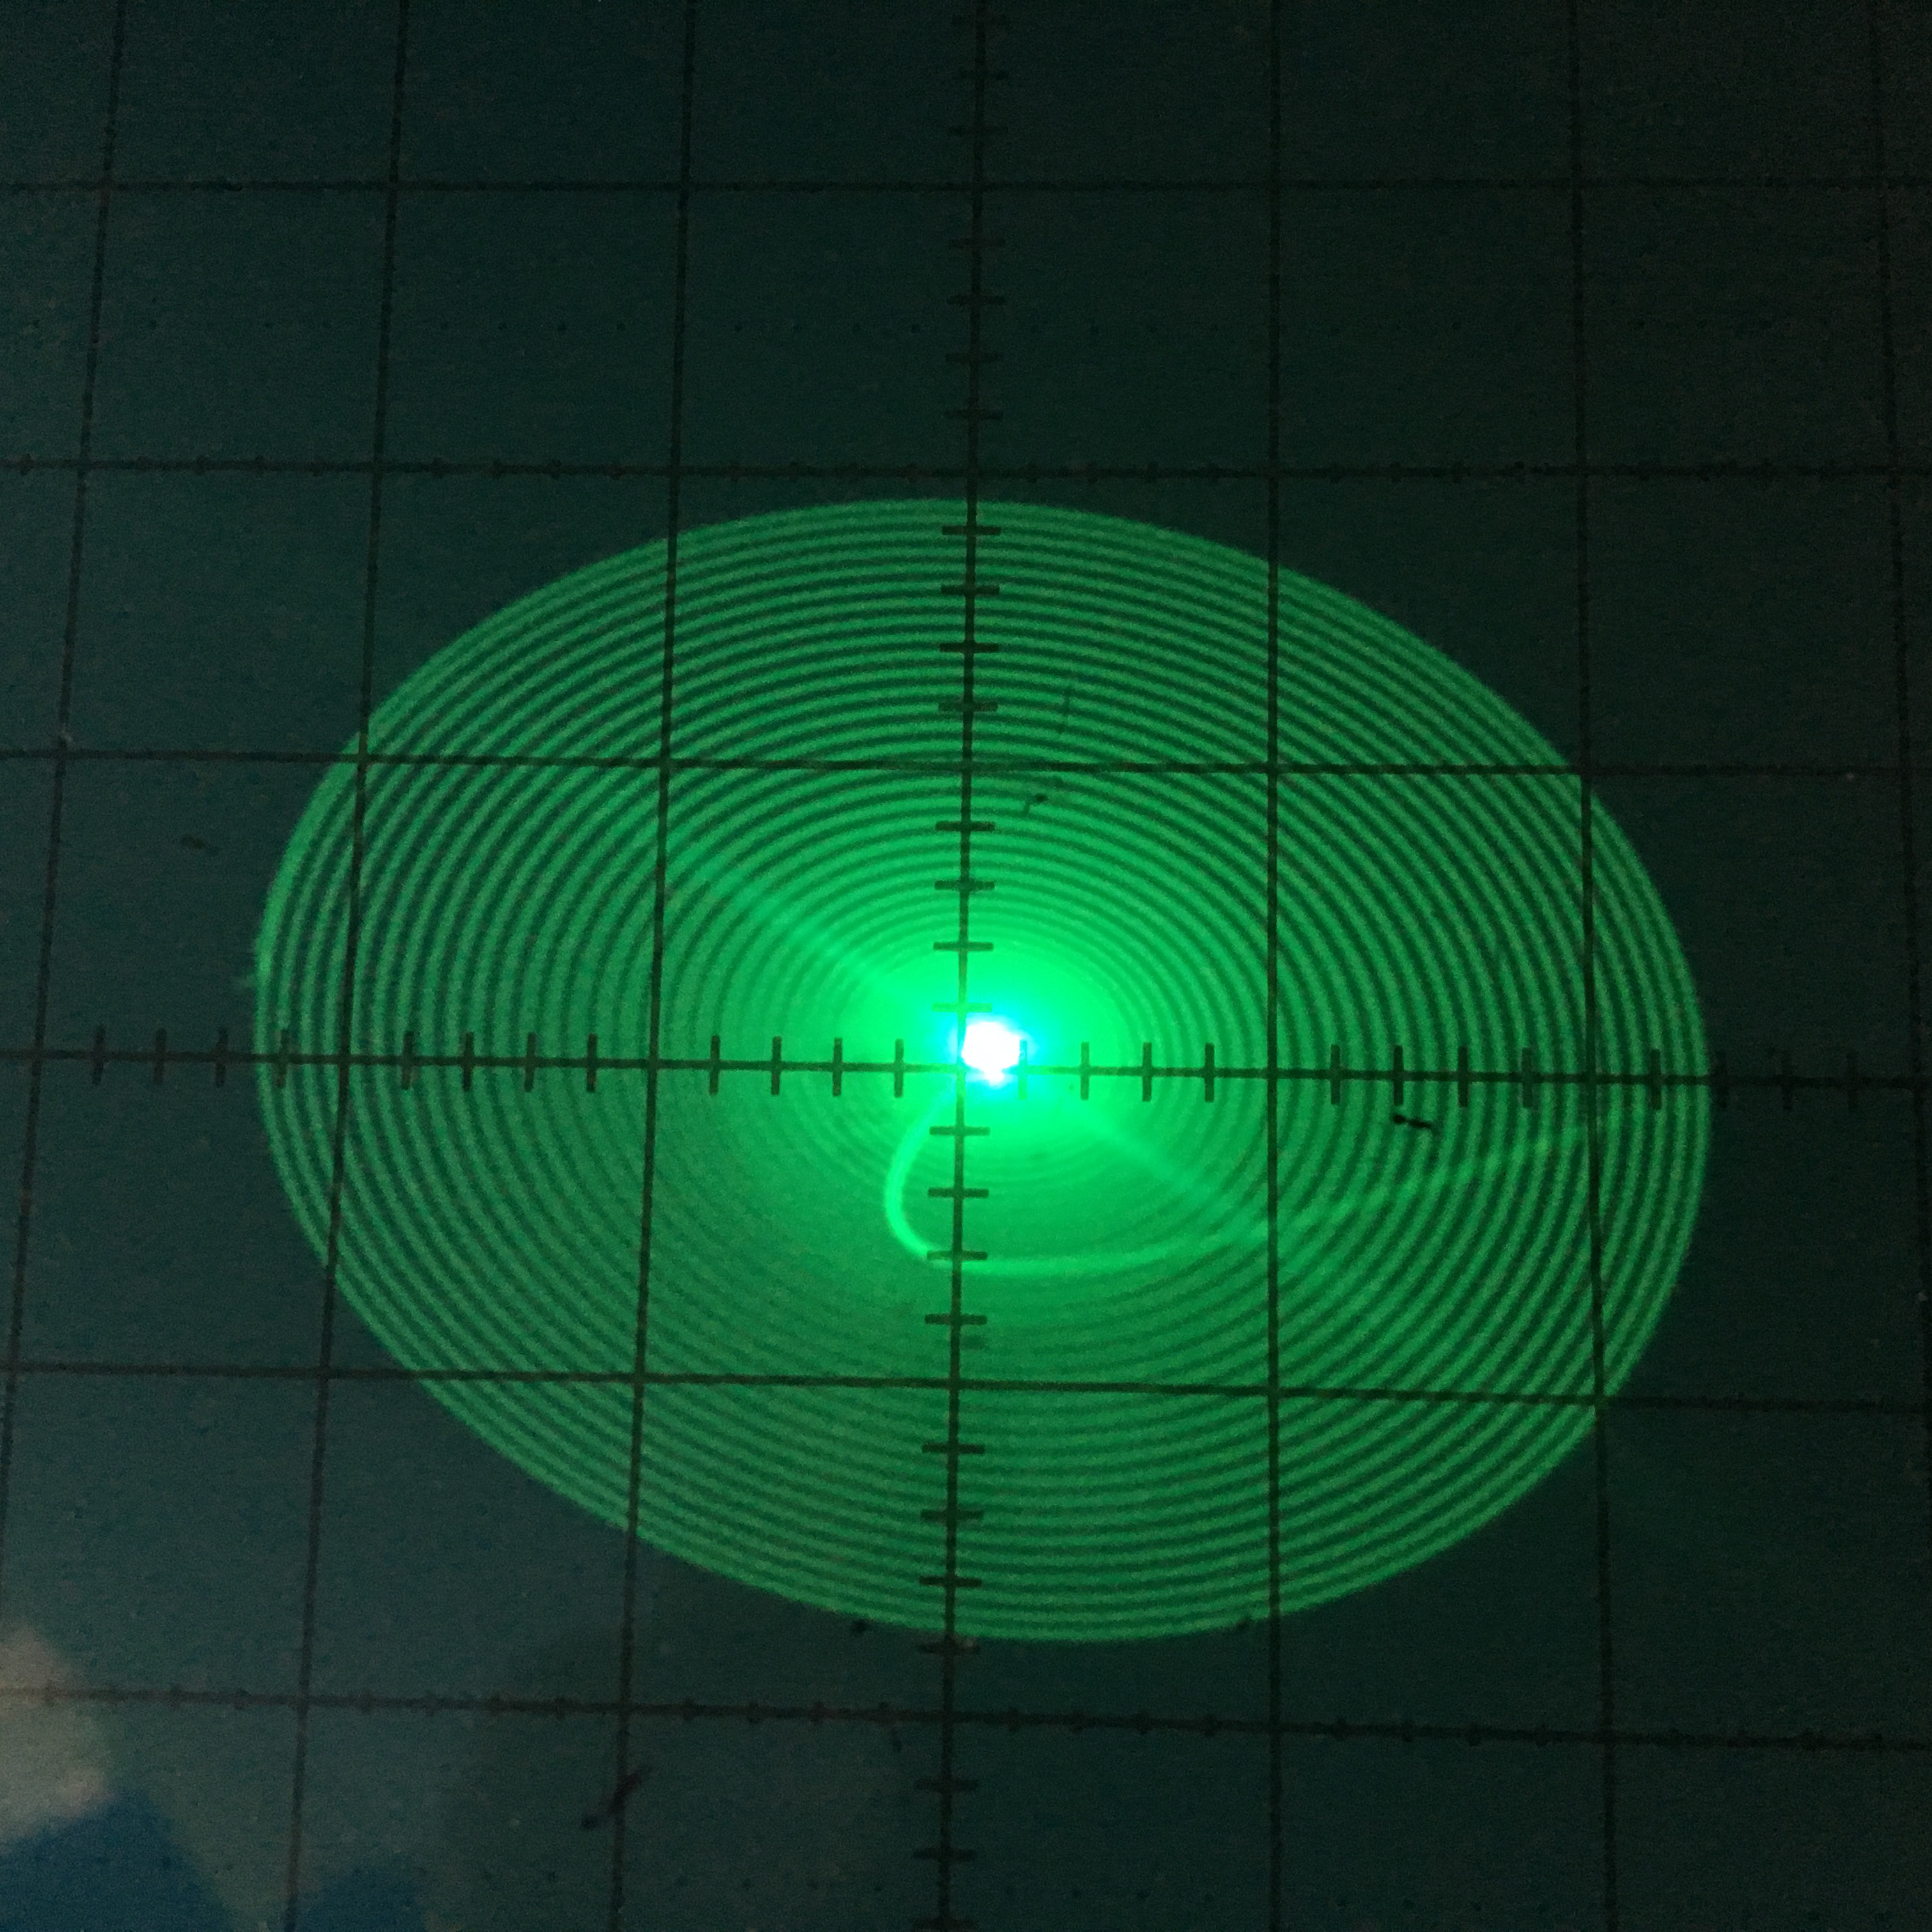
\includegraphics[width=\linewidth]{photo/task2c(leftL).jpg}
	\end{minipage}
	\caption{Фазовые траектории при $M<M'$}
	\label{fig9}
\end{figure}
\vspace{-30pt}
\begin{figure}[h]
	\centering
	\begin{minipage}{0.32\linewidth}
	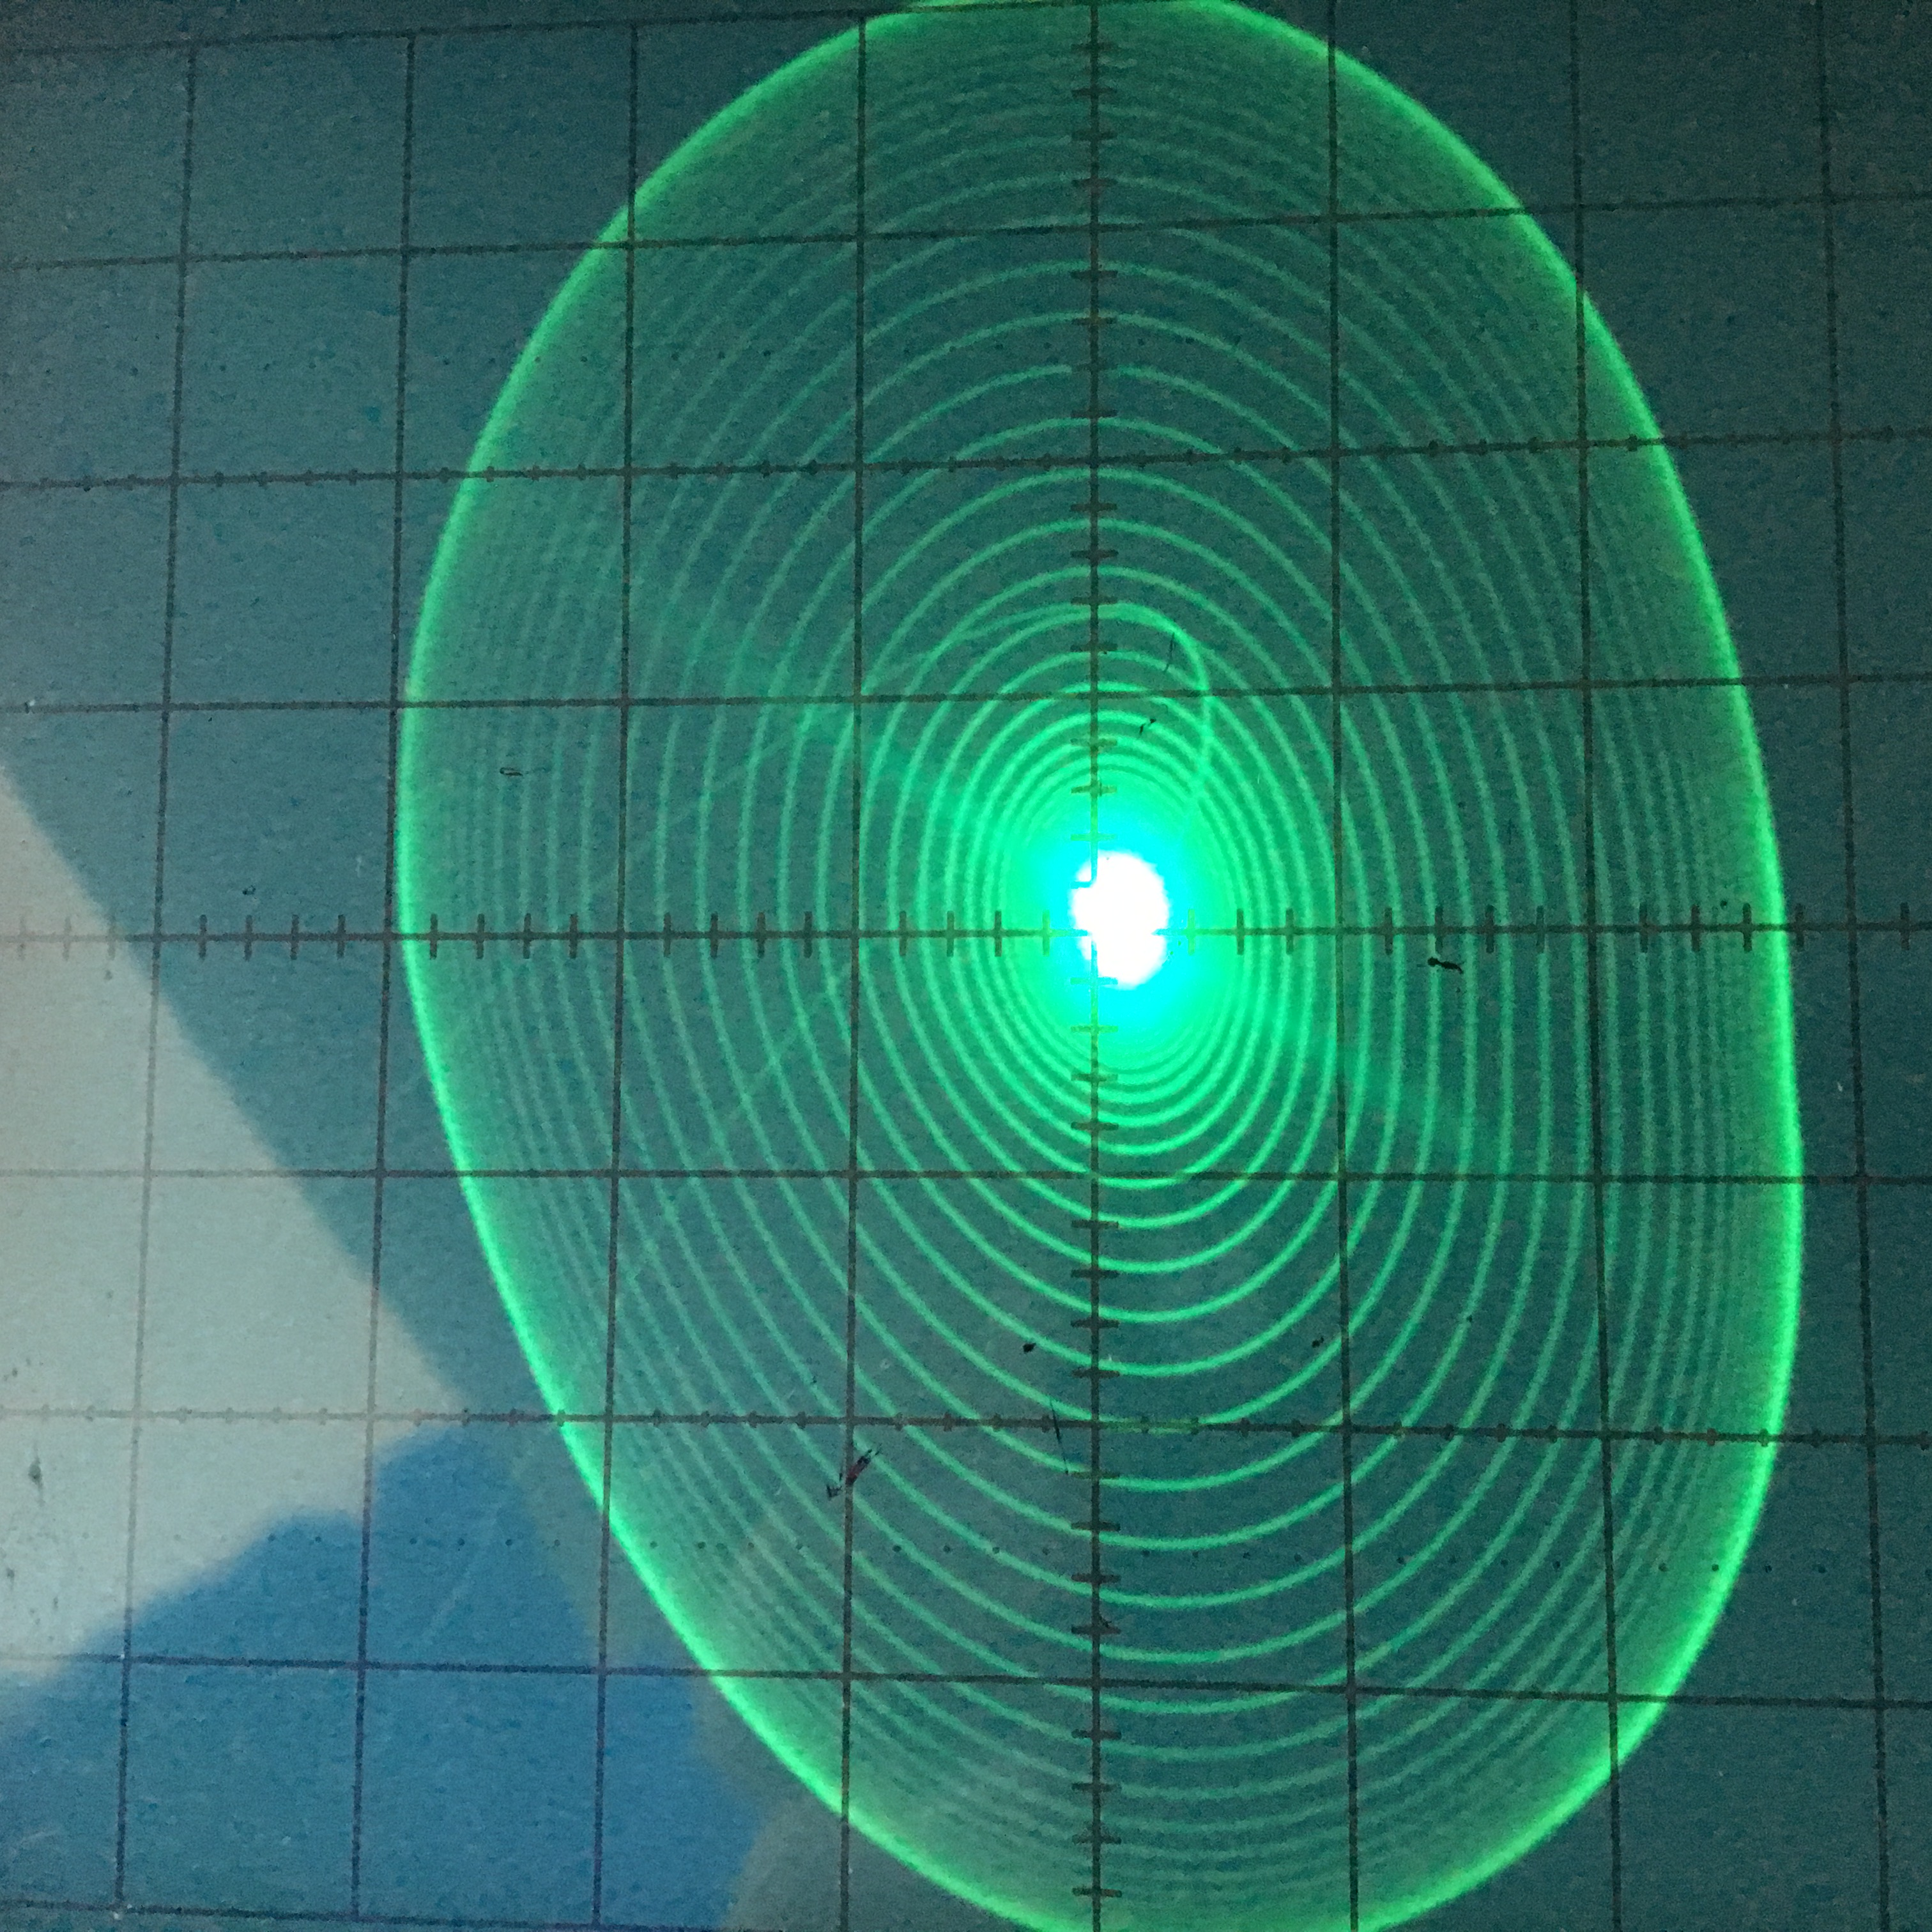
\includegraphics[width=\linewidth]{photo/task2c(mids).jpg}
	\end{minipage}
	\begin{minipage}{0.32\linewidth}
	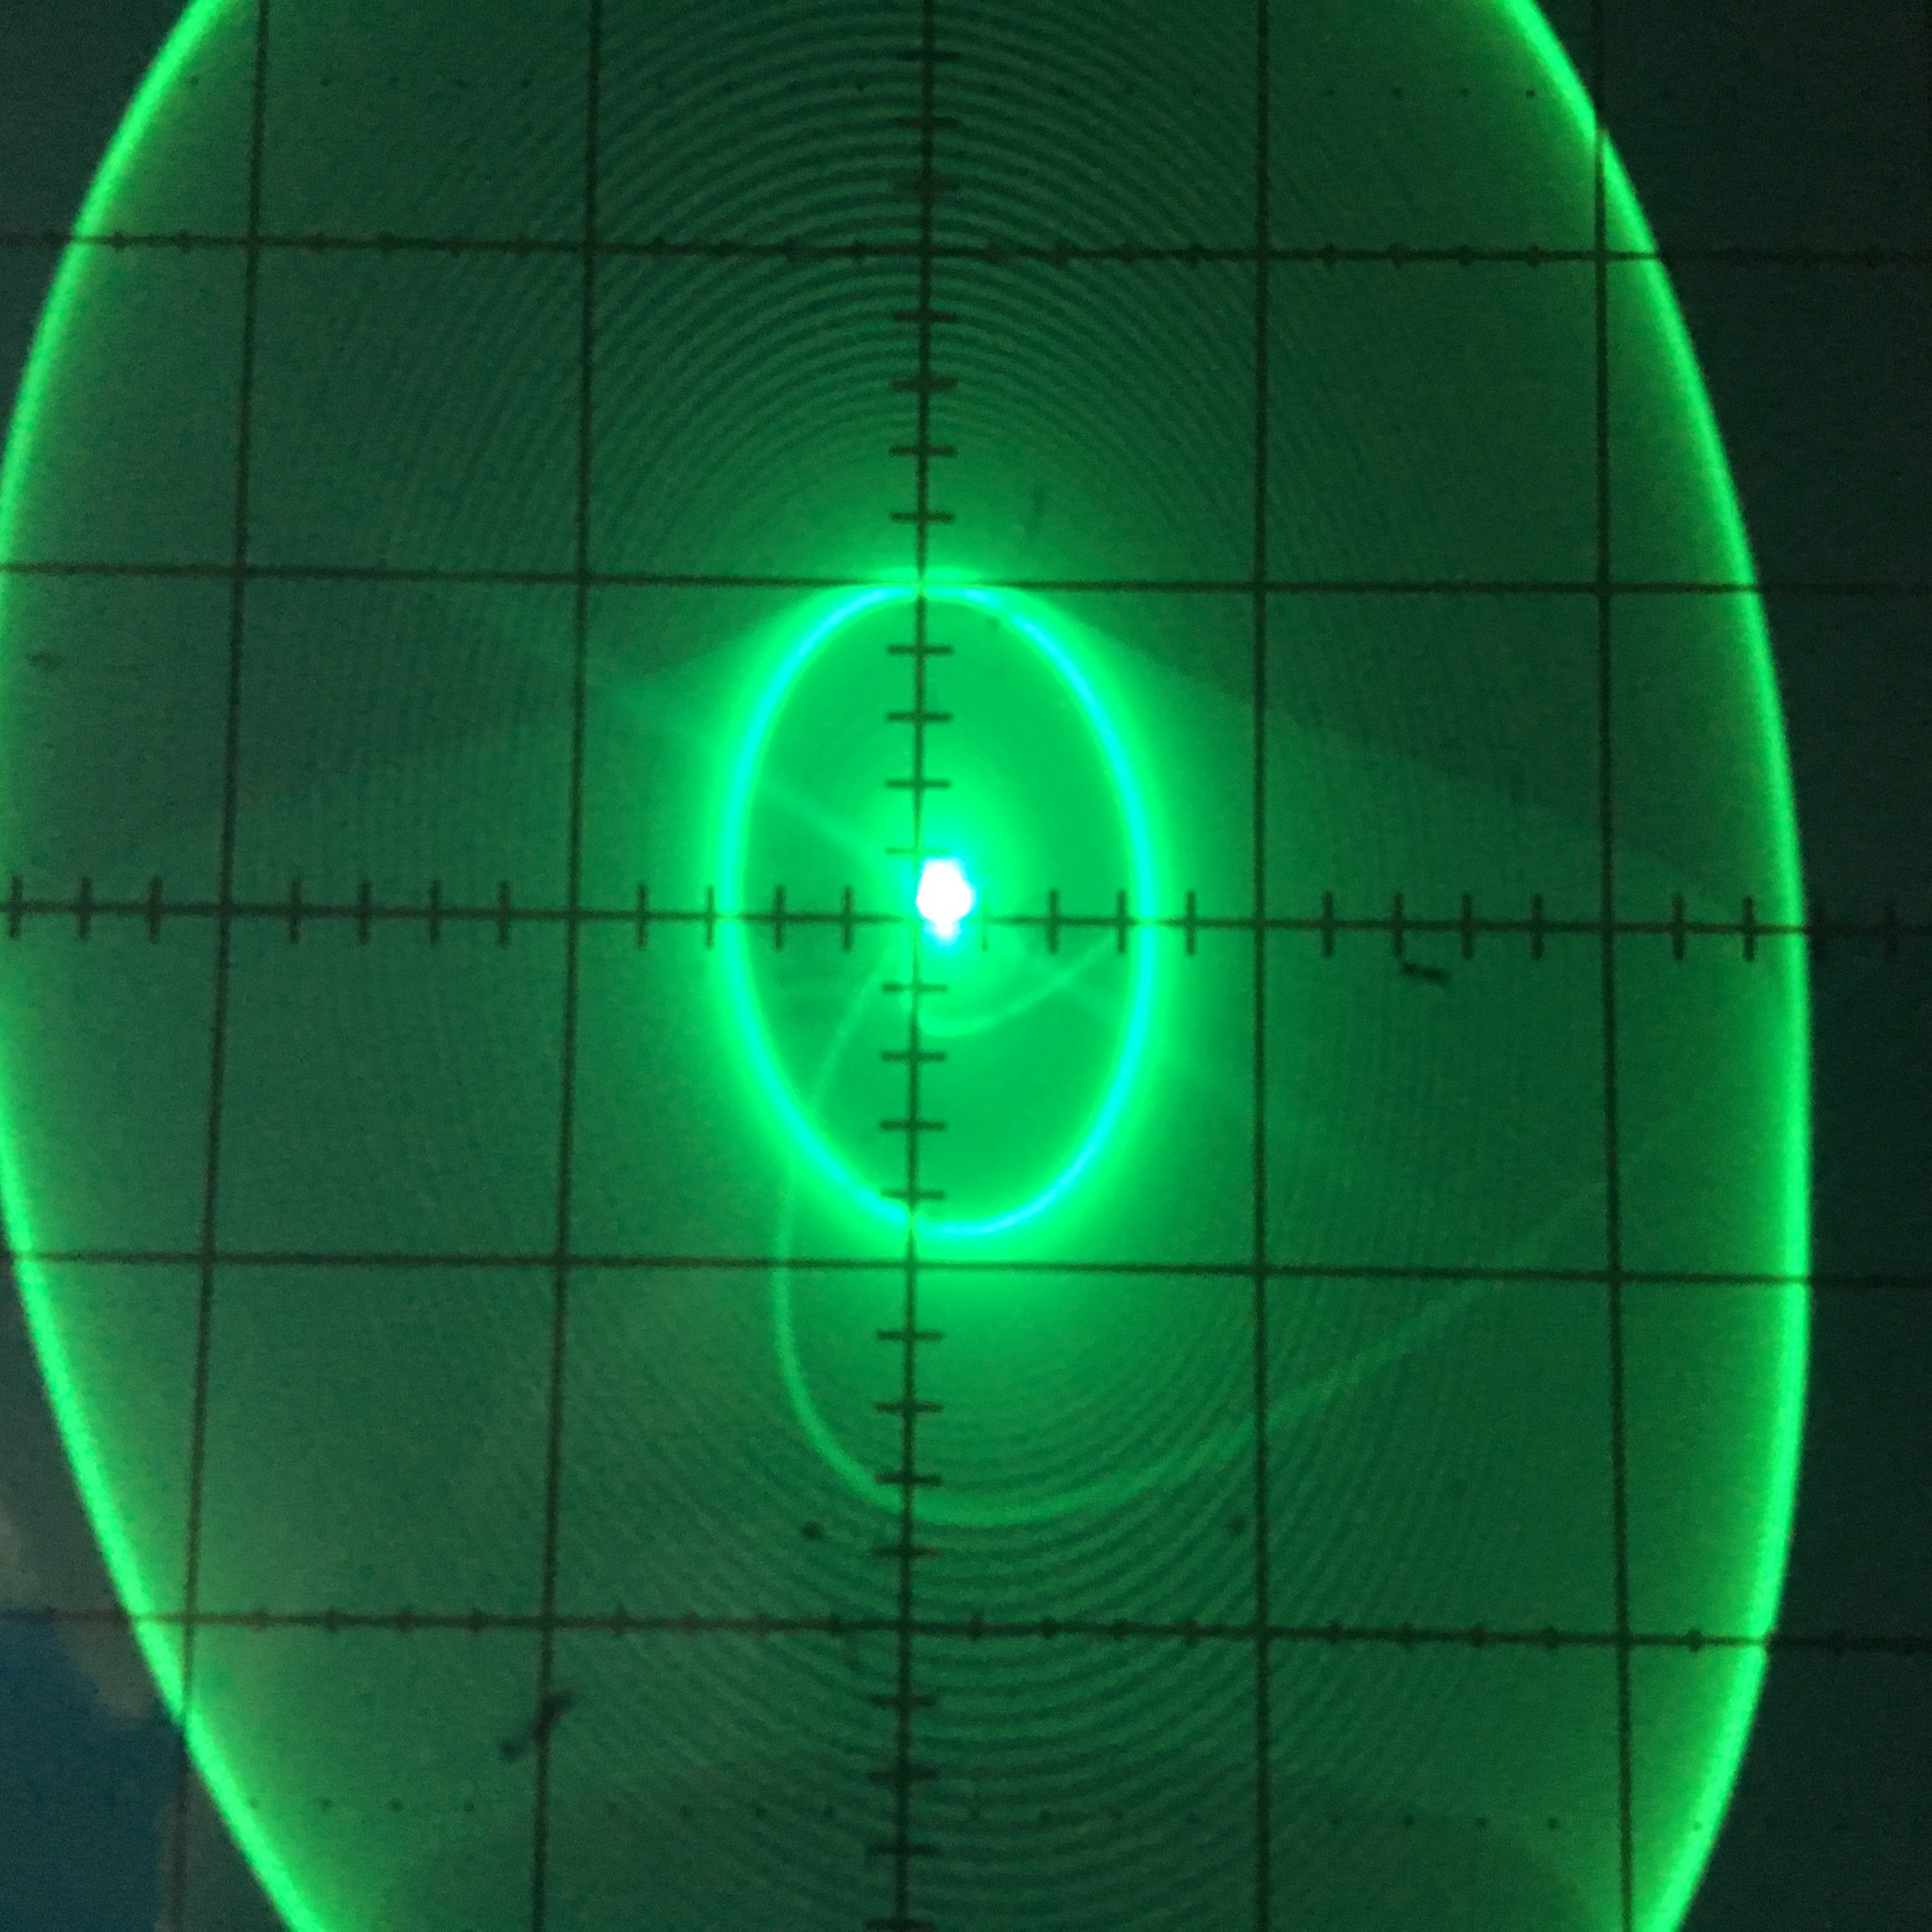
\includegraphics[width=\linewidth]{photo/task2c(midm).jpg}
	\end{minipage}
	\begin{minipage}{0.32\linewidth}
	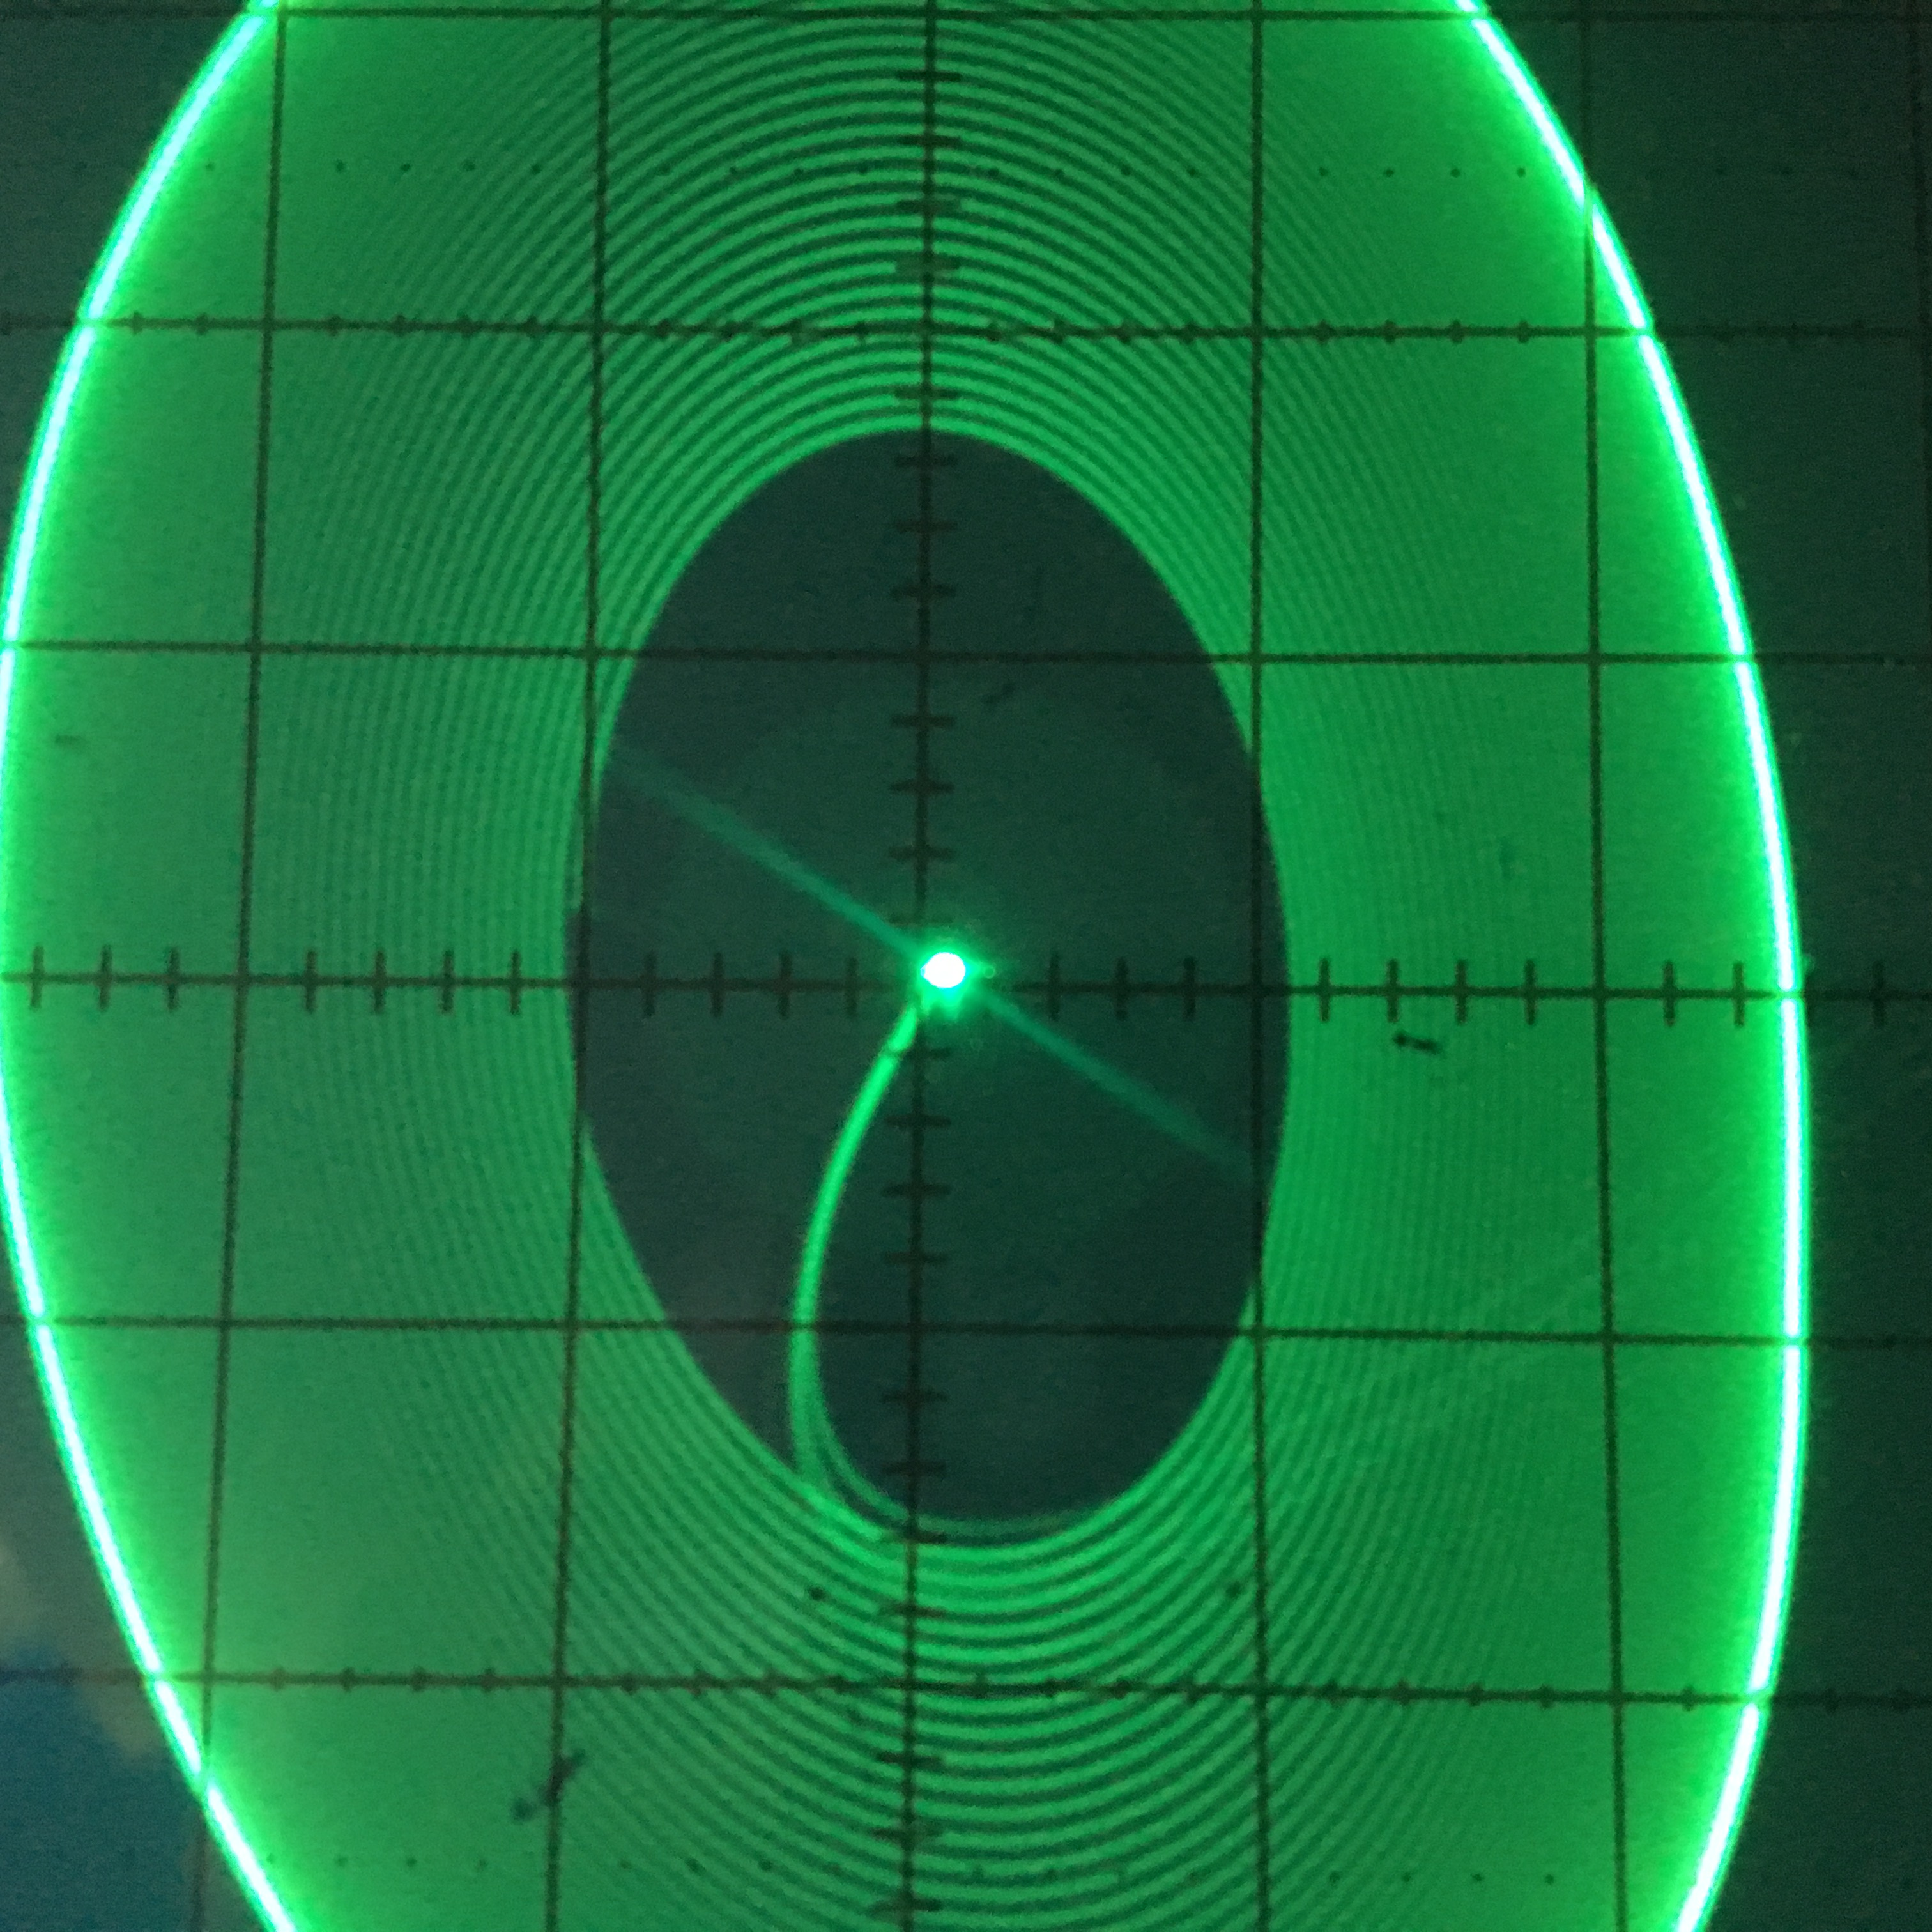
\includegraphics[width=\linewidth]{photo/task2c(midL).jpg}
	\end{minipage}
	\caption{Фазовые траектории при $M'<M<M''$}
	\label{fig10}
\end{figure}
\vspace{-30pt}
\begin{figure}[h!]
	\centering
	\begin{minipage}{0.32\linewidth}
	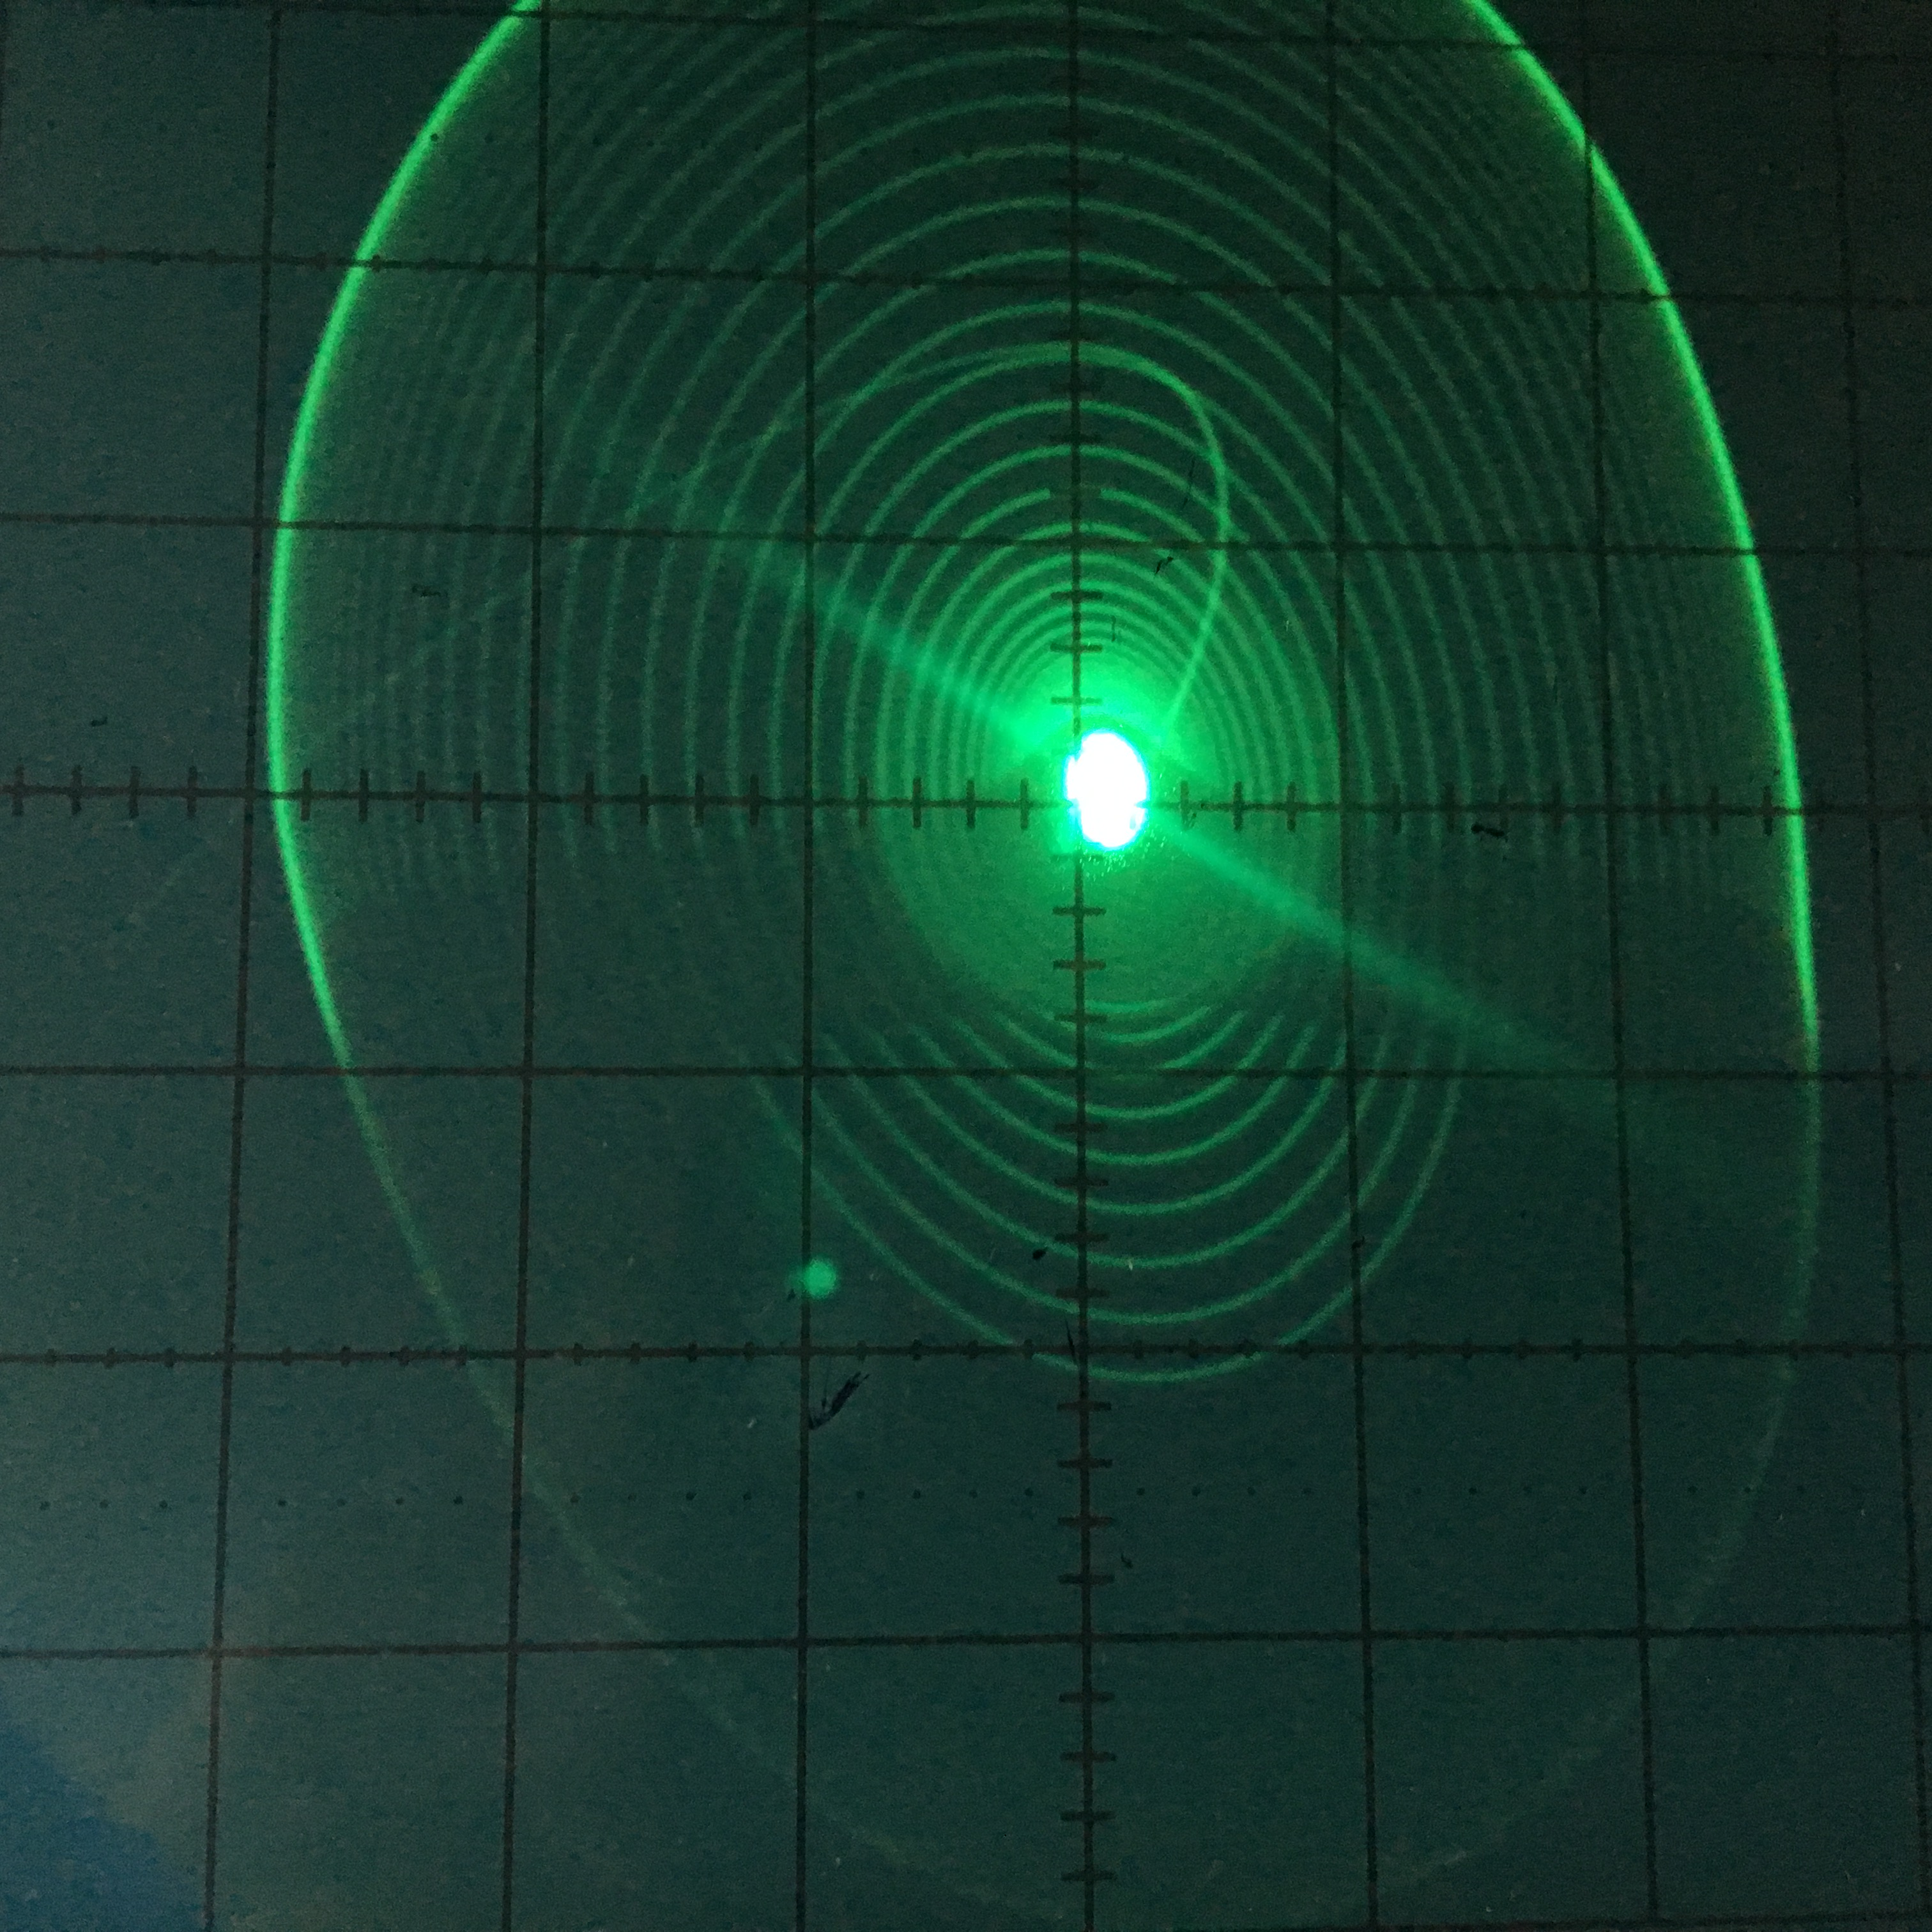
\includegraphics[width=\linewidth]{photo/task2c(rights).jpg}
	\end{minipage}
	\begin{minipage}{0.32\linewidth}
	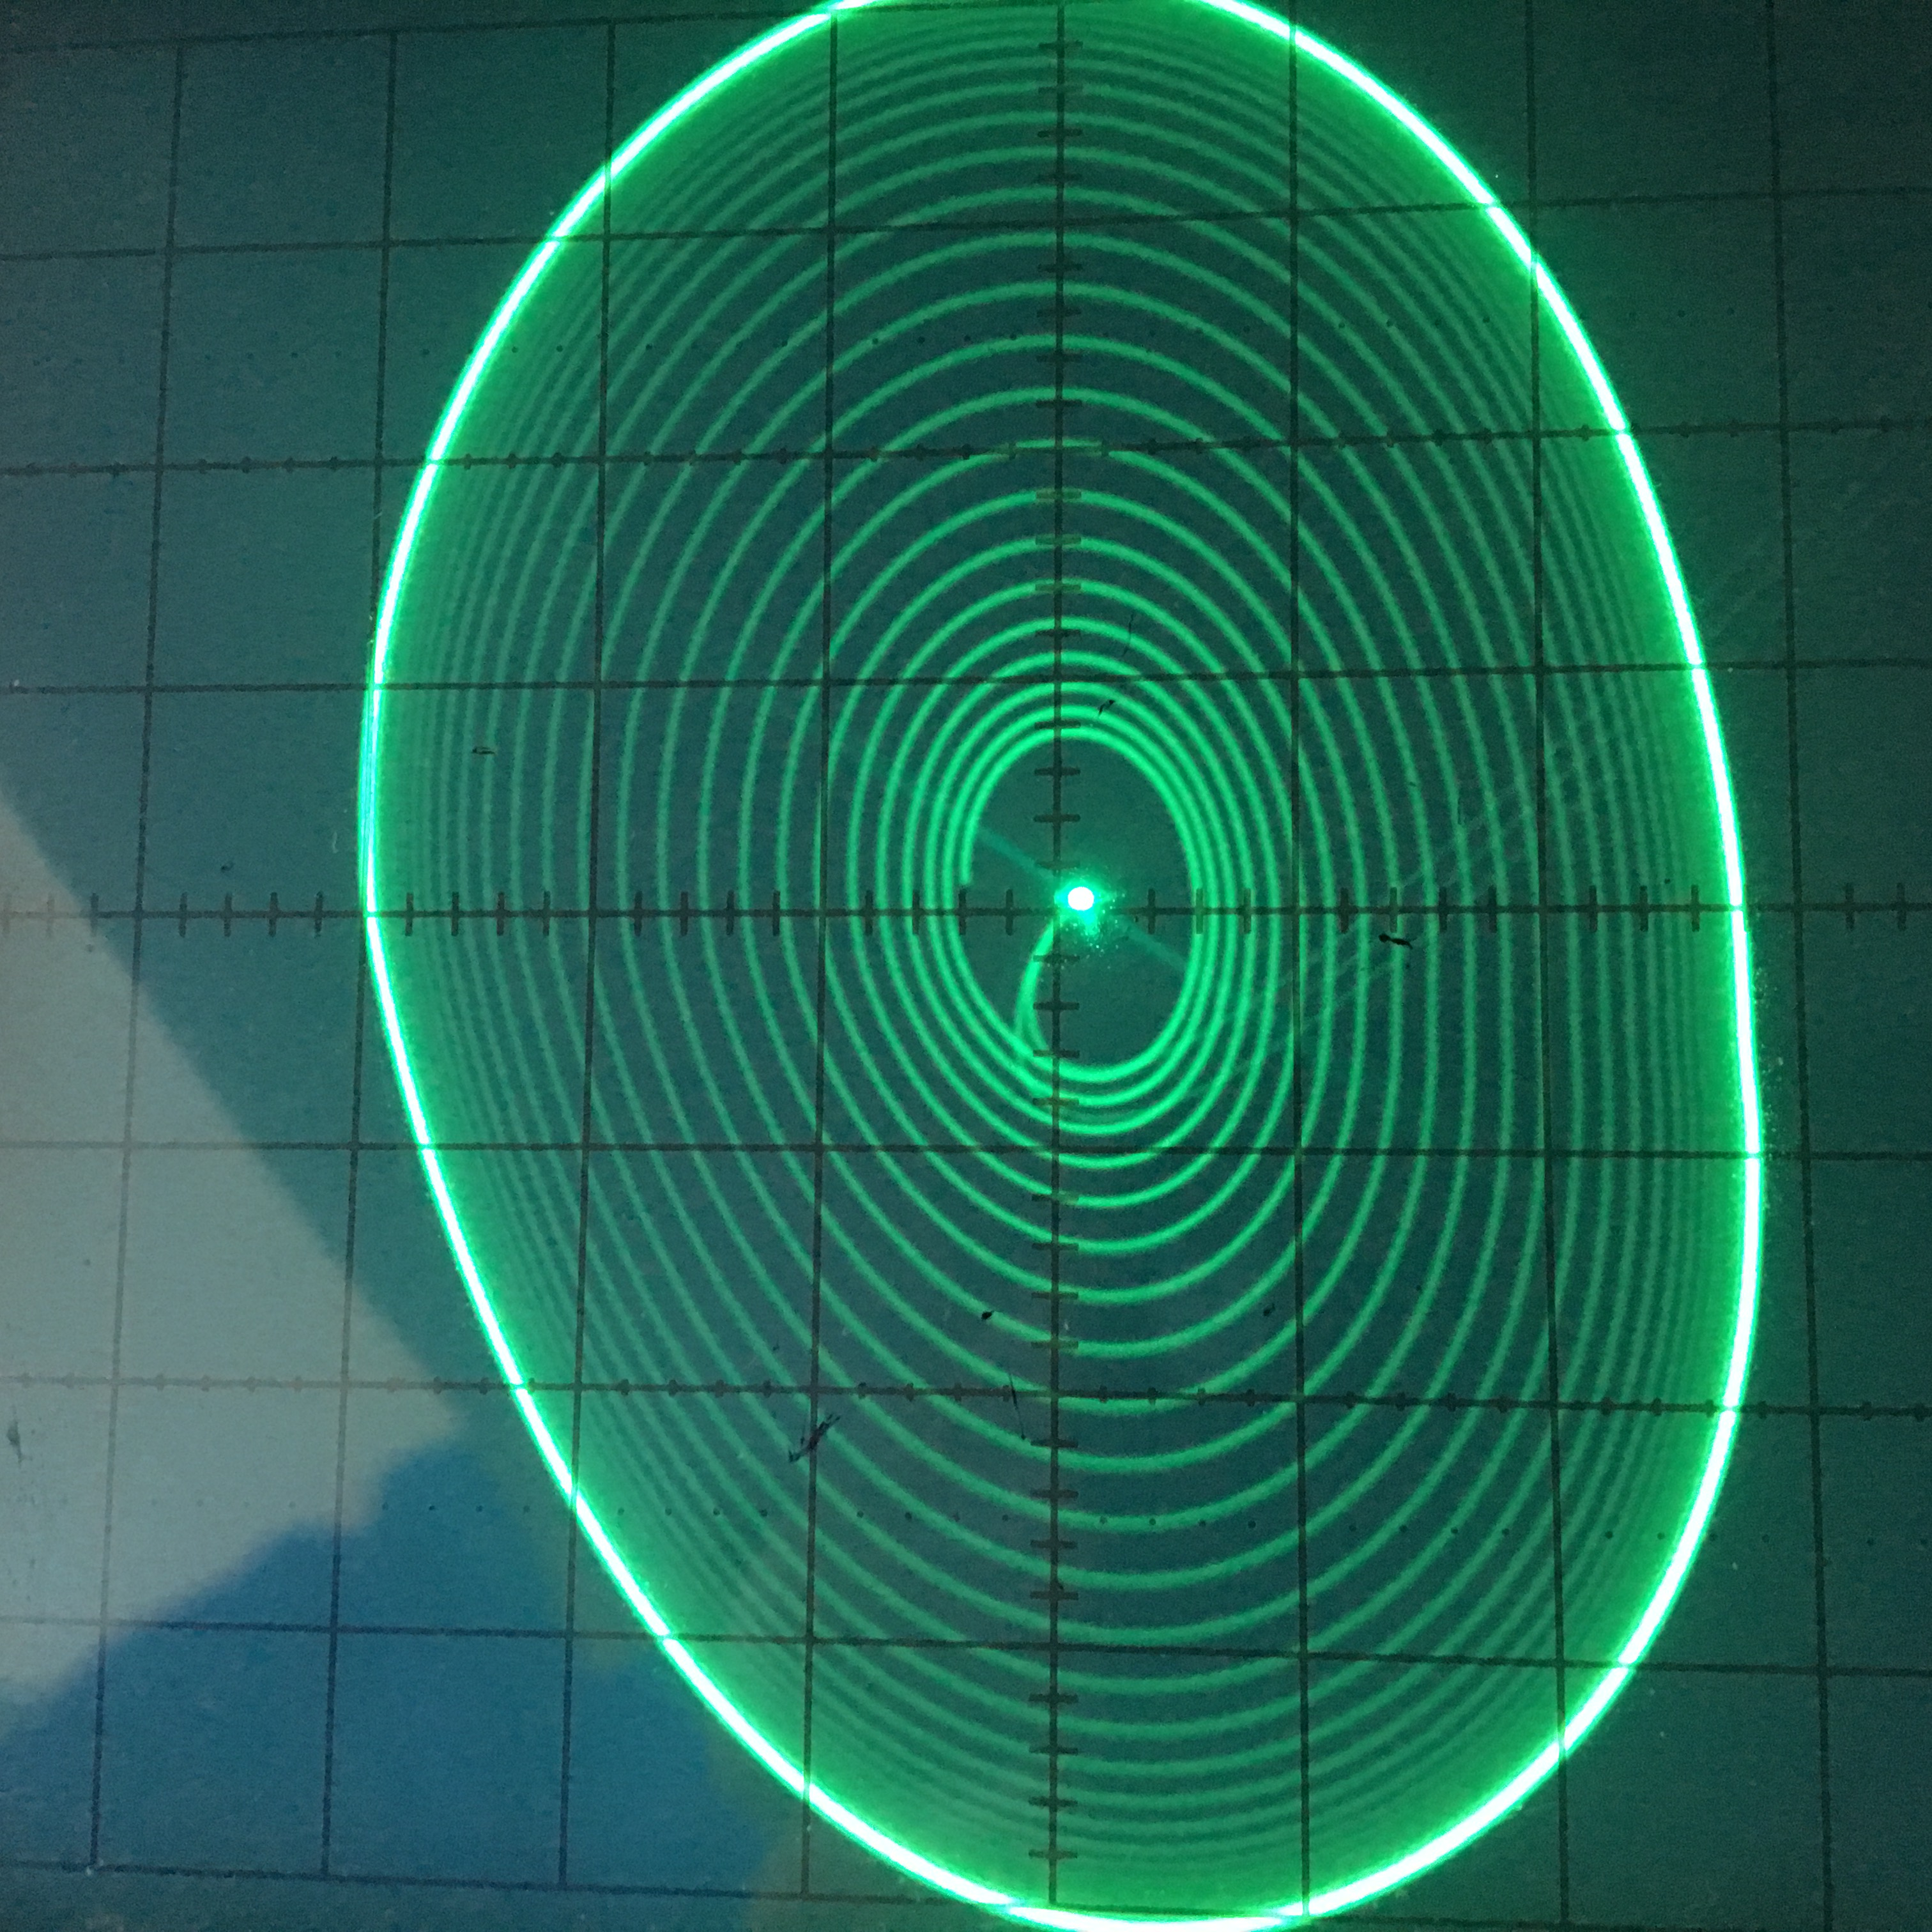
\includegraphics[width=\linewidth]{photo/task2c(rightm).jpg}
	\end{minipage}
	\caption{Фазовые траектории при $M>M''$}
	\label{fig11}
\end{figure}
\subsection{Сложно-жесткий режим генератора}
\subsubsection{Бифрукационная диаграмма}
Сняли бифуркационную диаграмму, выражающую зависимость амплитуды автоколебаний от величины взаимоиндукции $M$.
\begin{figure}[h]
	\centering
	\vspace{-10pt}
	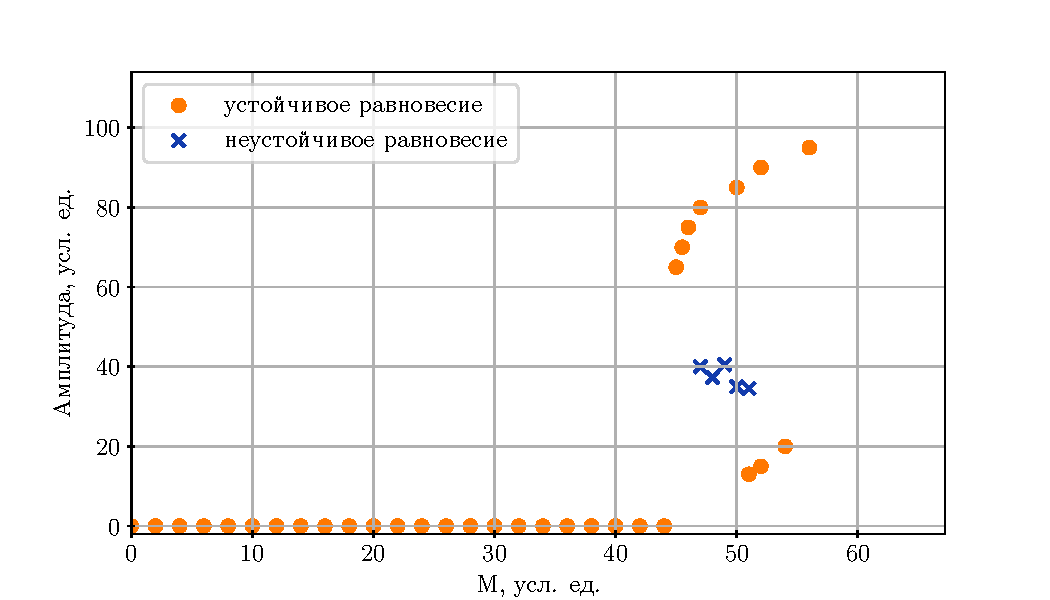
\includegraphics[]{plots/veryharddiagram.pdf}
	\caption{бифрукационная диаграмма для cложно-жесткого режима}
	\label{fig12}
\end{figure}
В данном случае также можно наблюдать характерную кривую бифрукационной диаграммы для сложно-жесткого типа как на рис.\ref{}.
\subsubsection{Фазовые траектории}
\begin{figure}[h!]
	\centering
	\begin{minipage}{0.32\linewidth}
	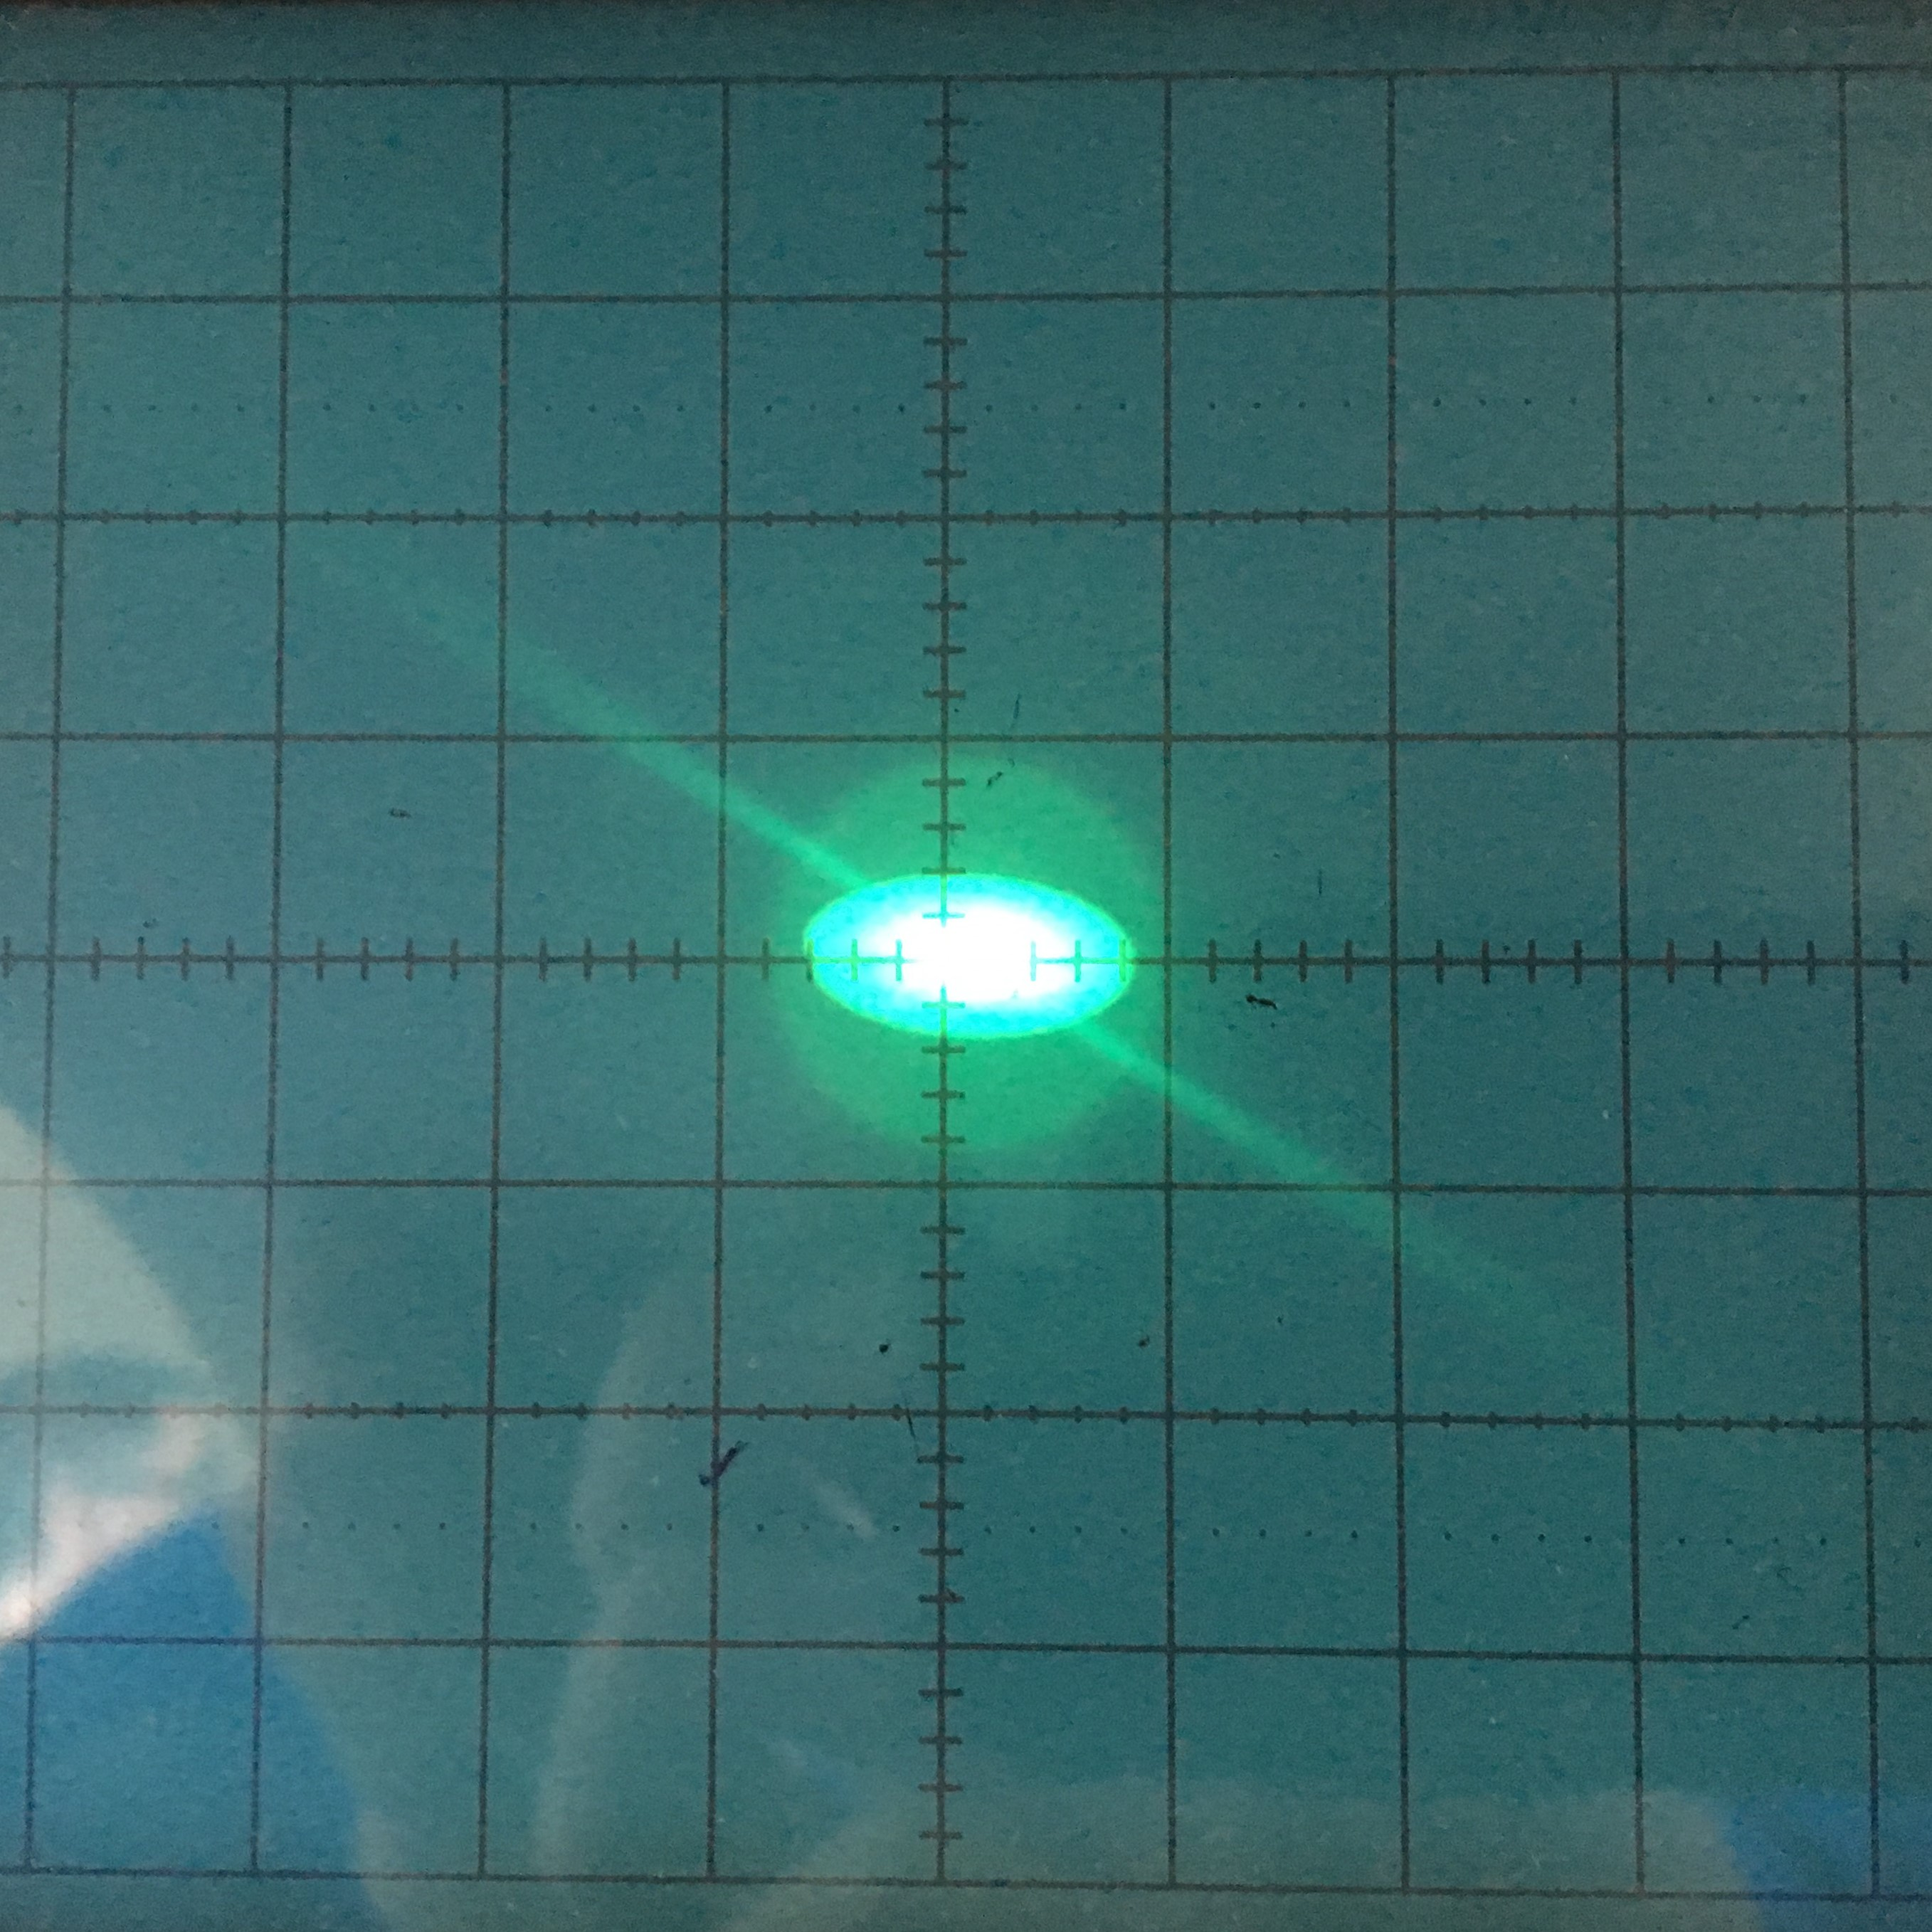
\includegraphics[width=\linewidth]{photo/task3b(lefts).jpg}
	\end{minipage}
	\begin{minipage}{0.32\linewidth}
	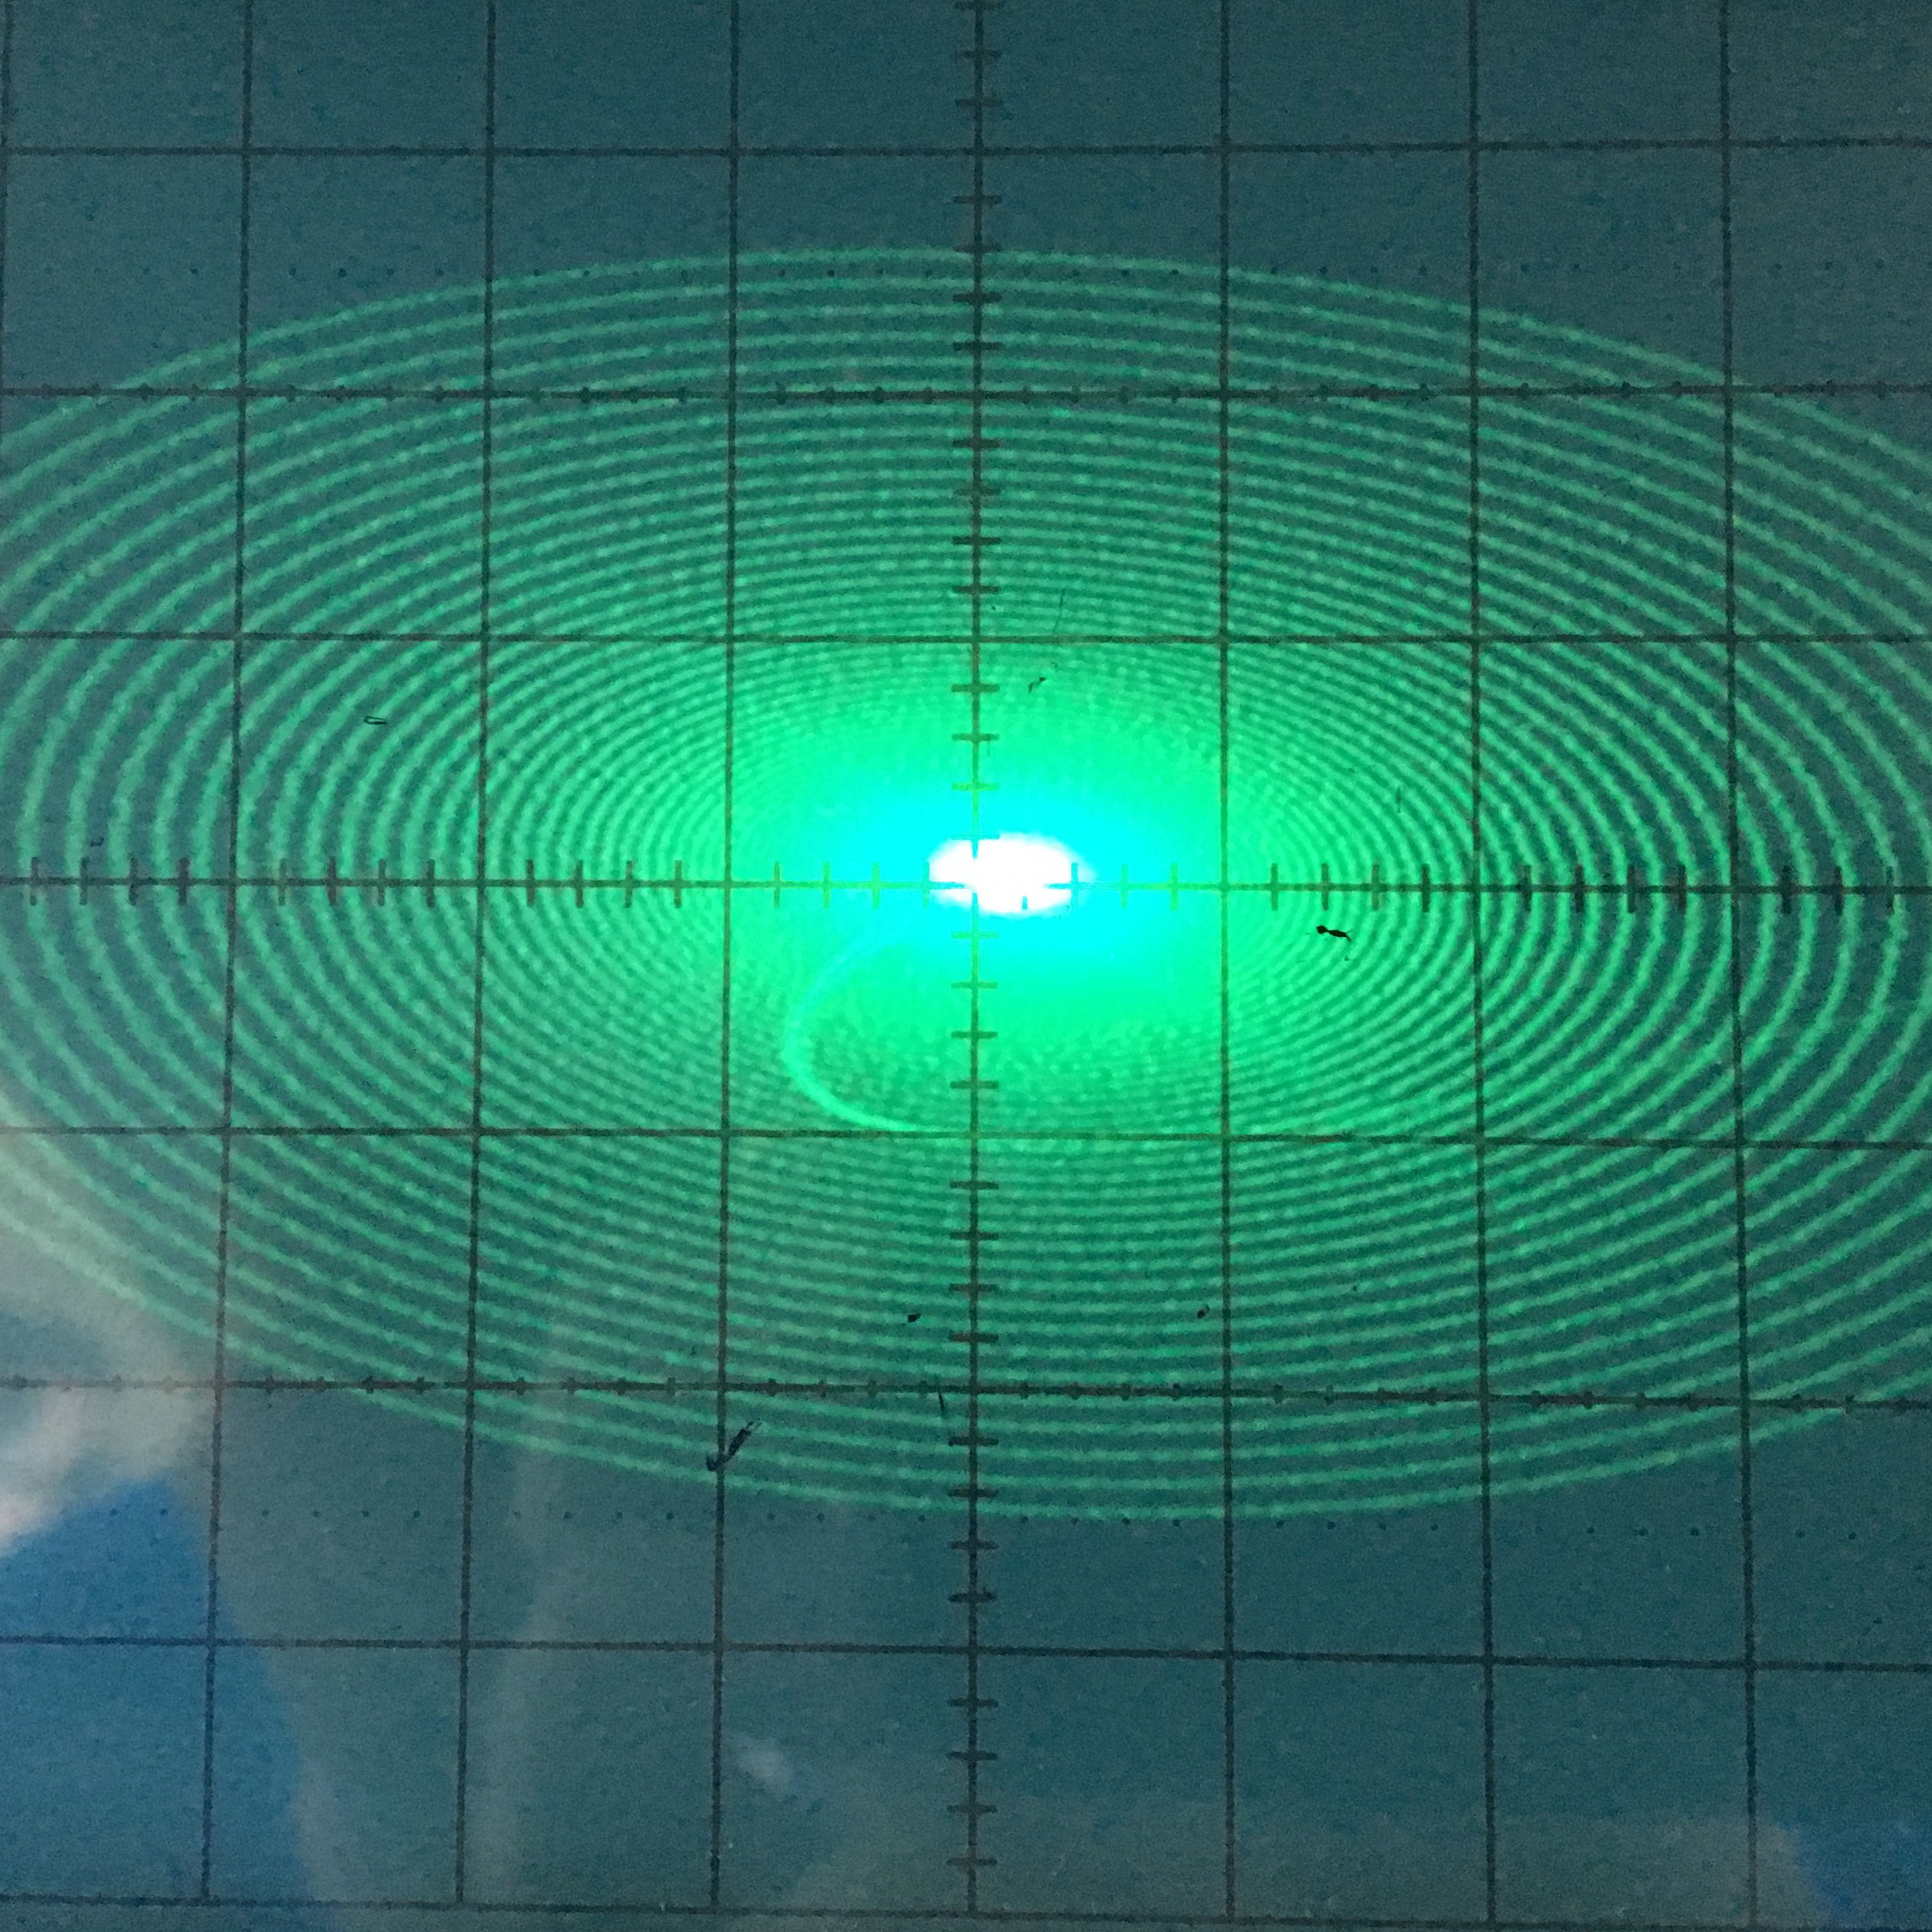
\includegraphics[width=\linewidth]{photo/task3b(leftm).jpg}
	\end{minipage}
	\begin{minipage}{0.32\linewidth}
	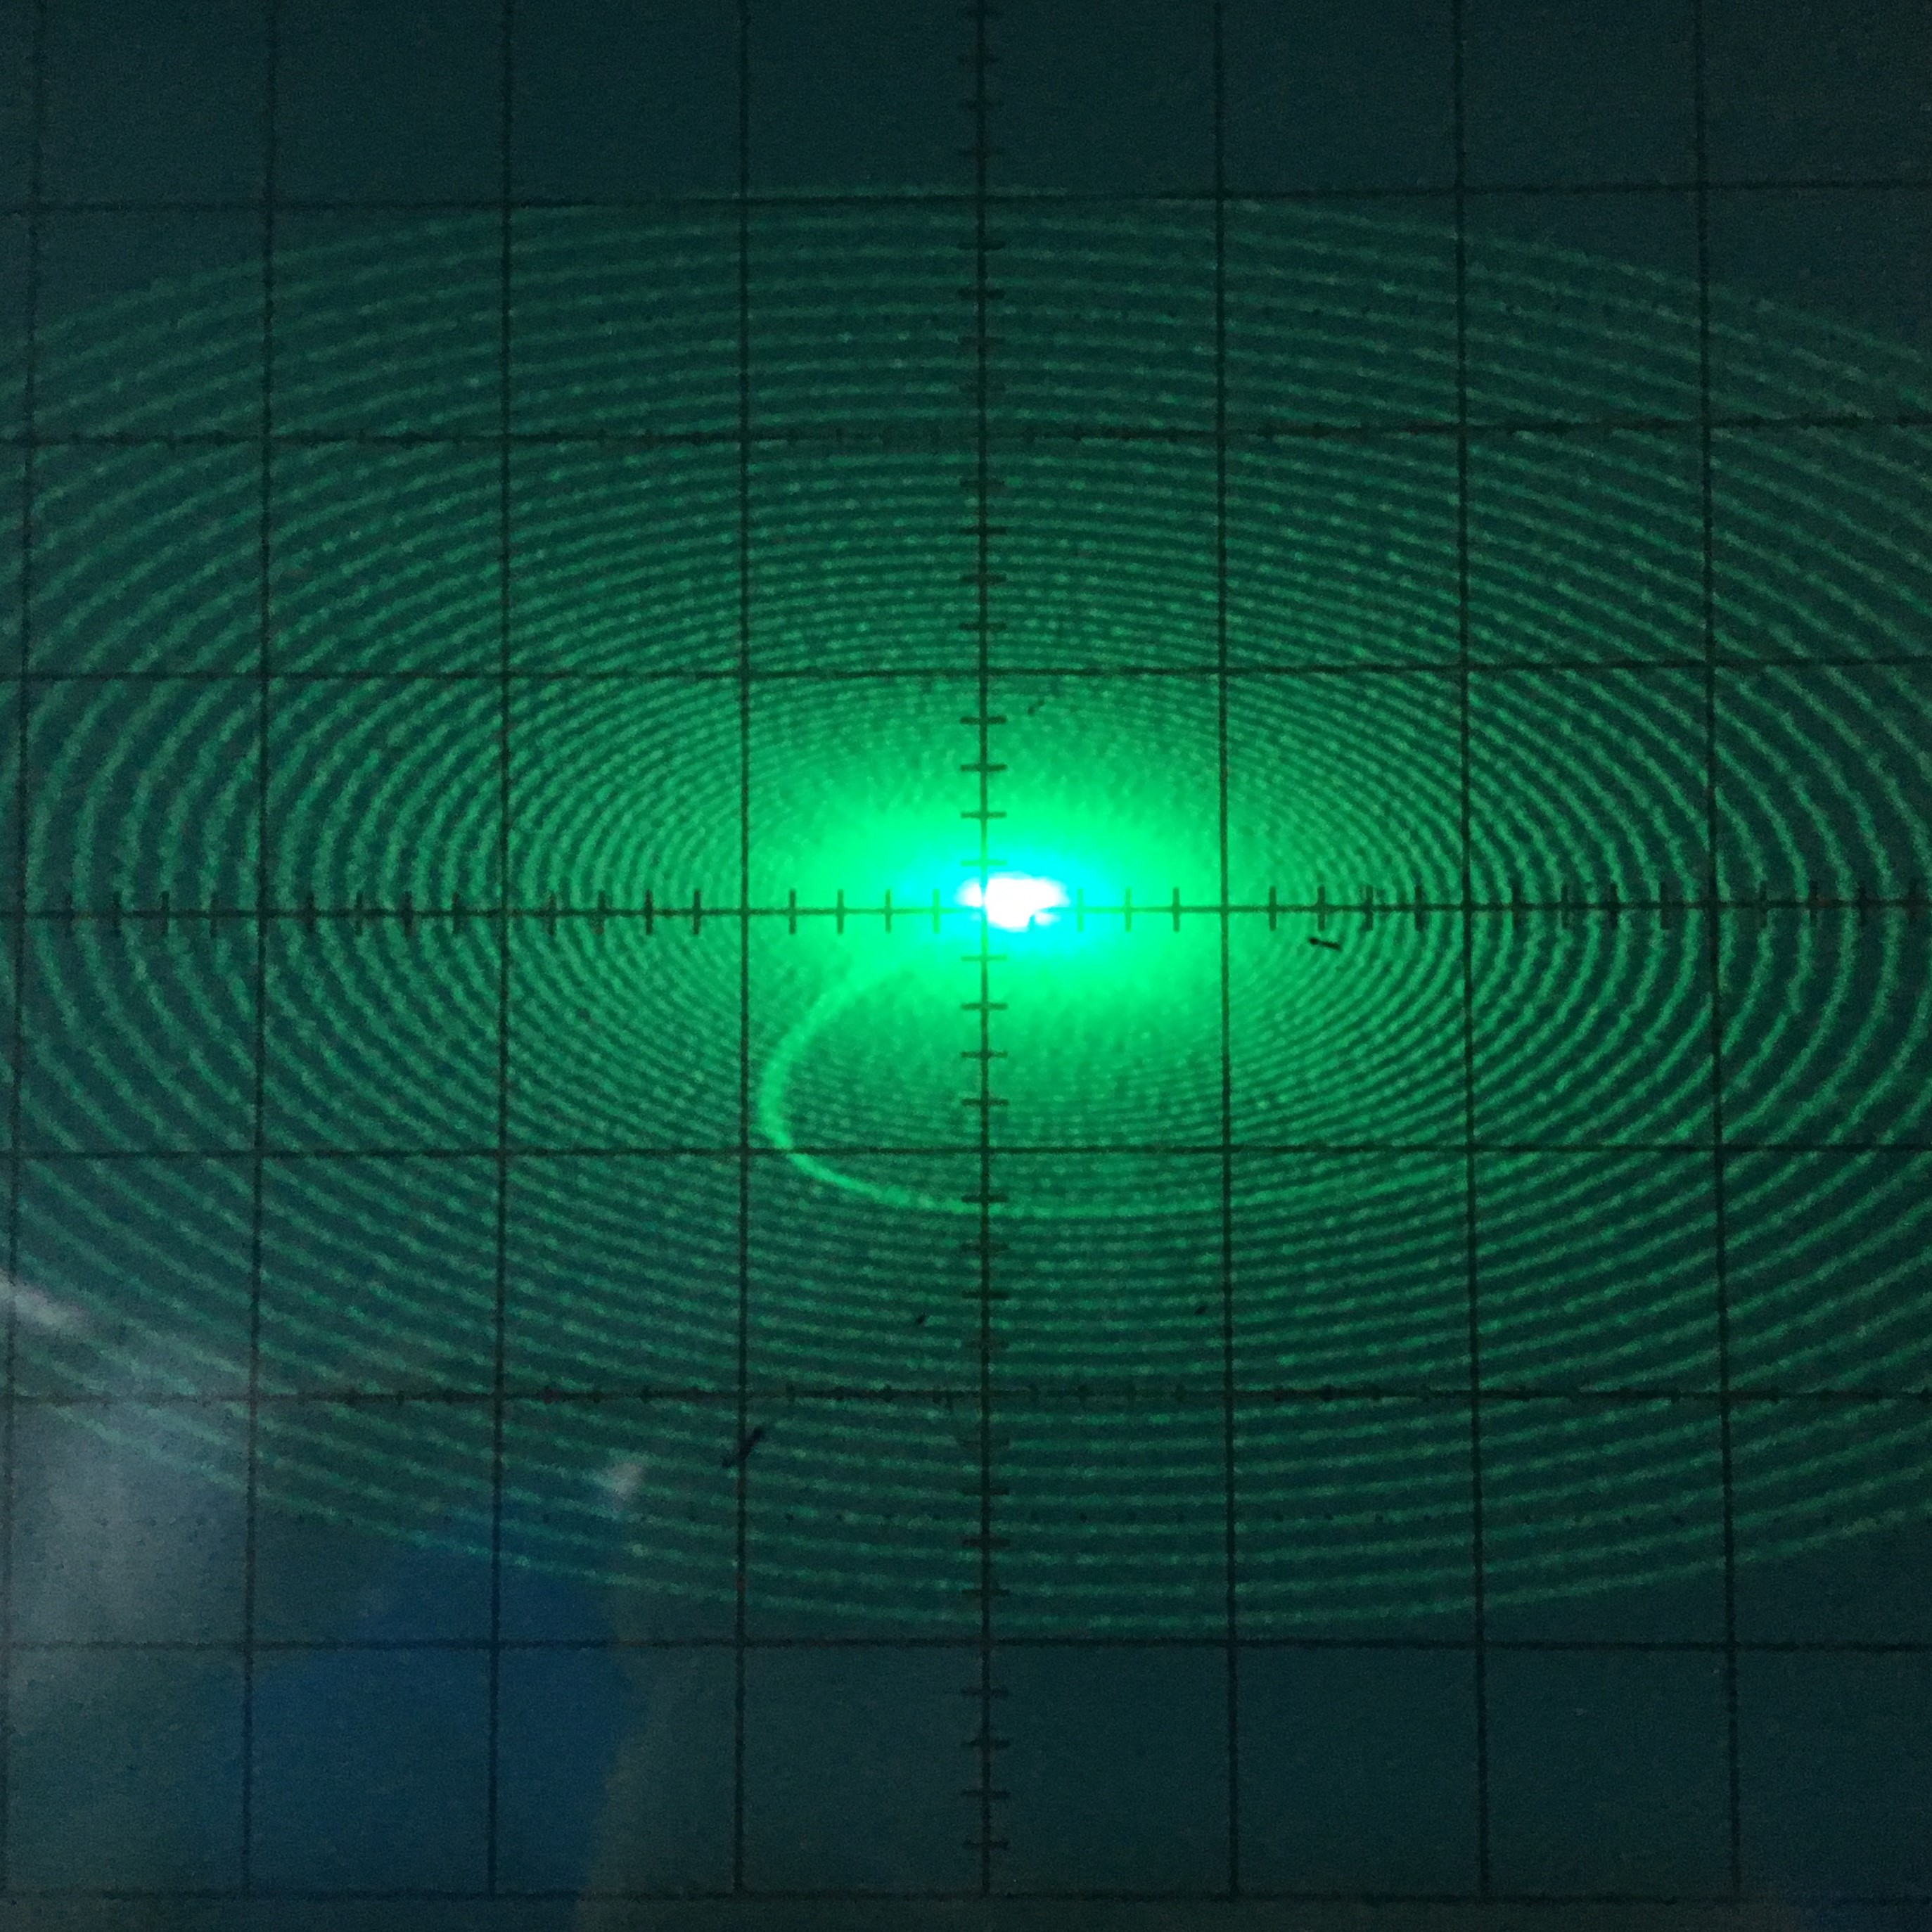
\includegraphics[width=\linewidth]{photo/task3b(leftL).jpg}
	\end{minipage}
	\caption{Фазовые траектории при $M<M'$}
	\label{fig13}
\end{figure}
\vspace{-20pt}
\begin{figure}[h!]
	\centering
	\vspace{-10pt}
	\begin{minipage}{0.32\linewidth}
	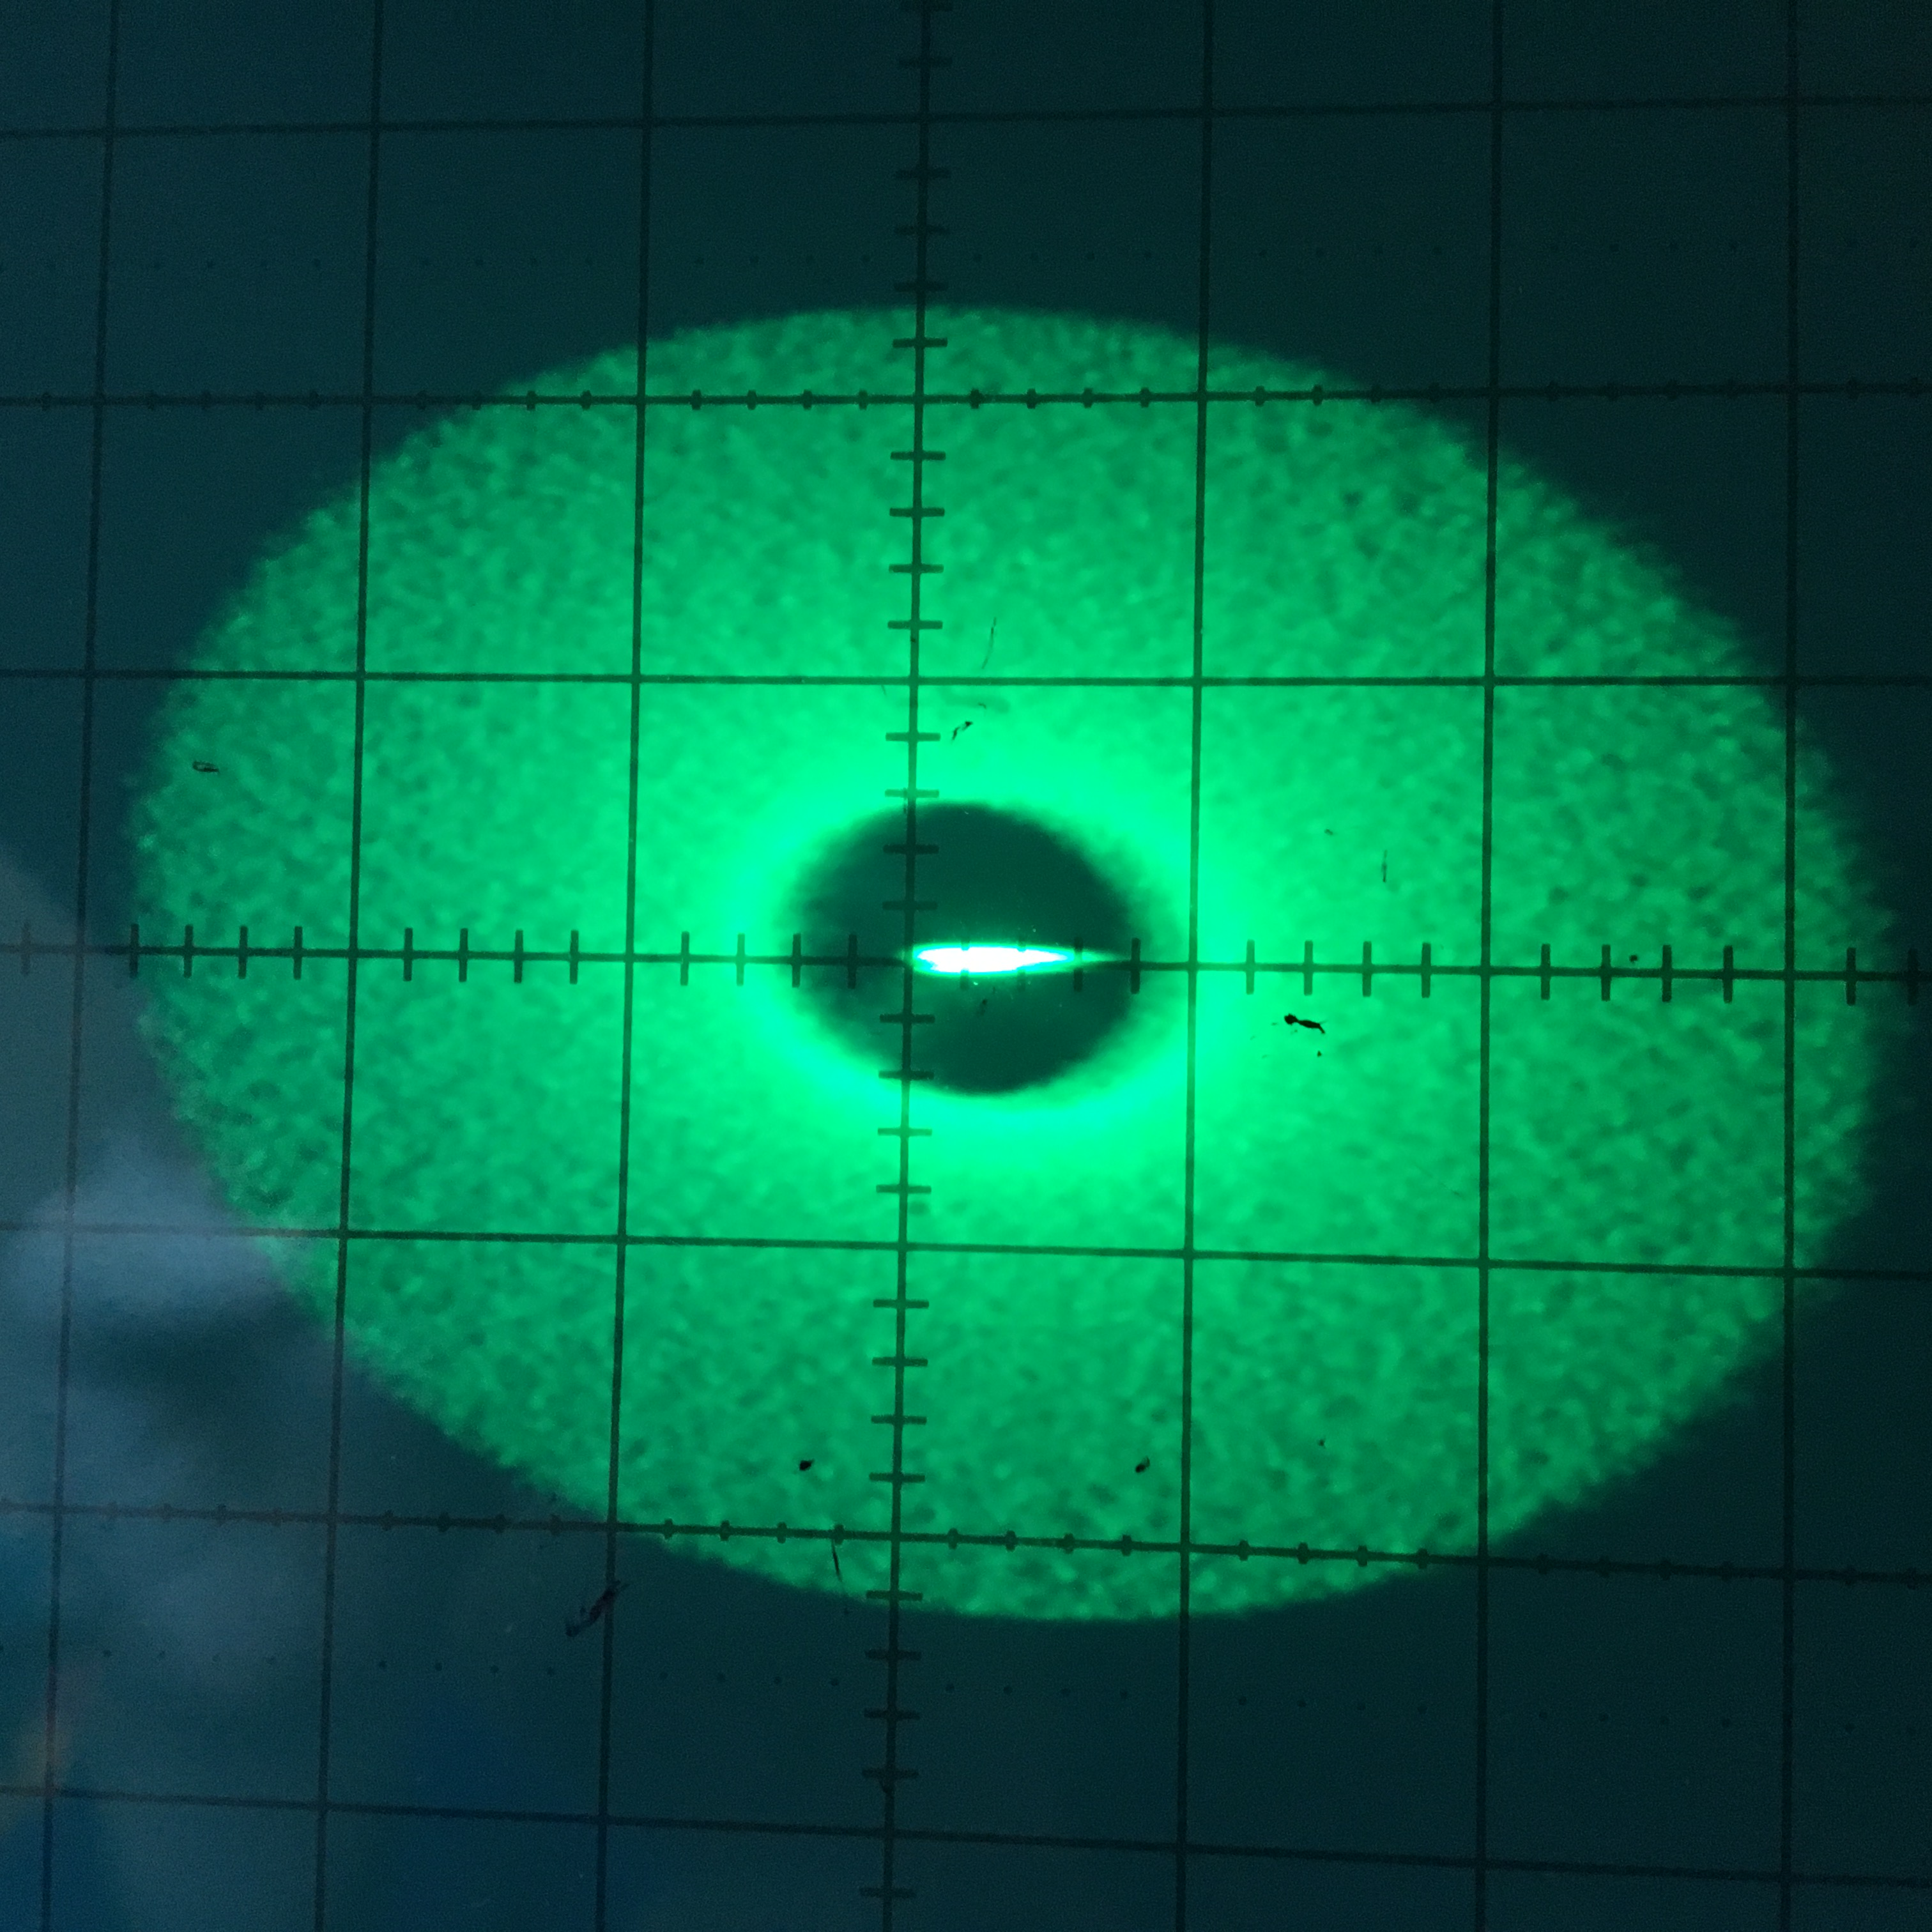
\includegraphics[width=\linewidth]{photo/task3b(mids).jpg}
	\end{minipage}
	\begin{minipage}{0.32\linewidth}
	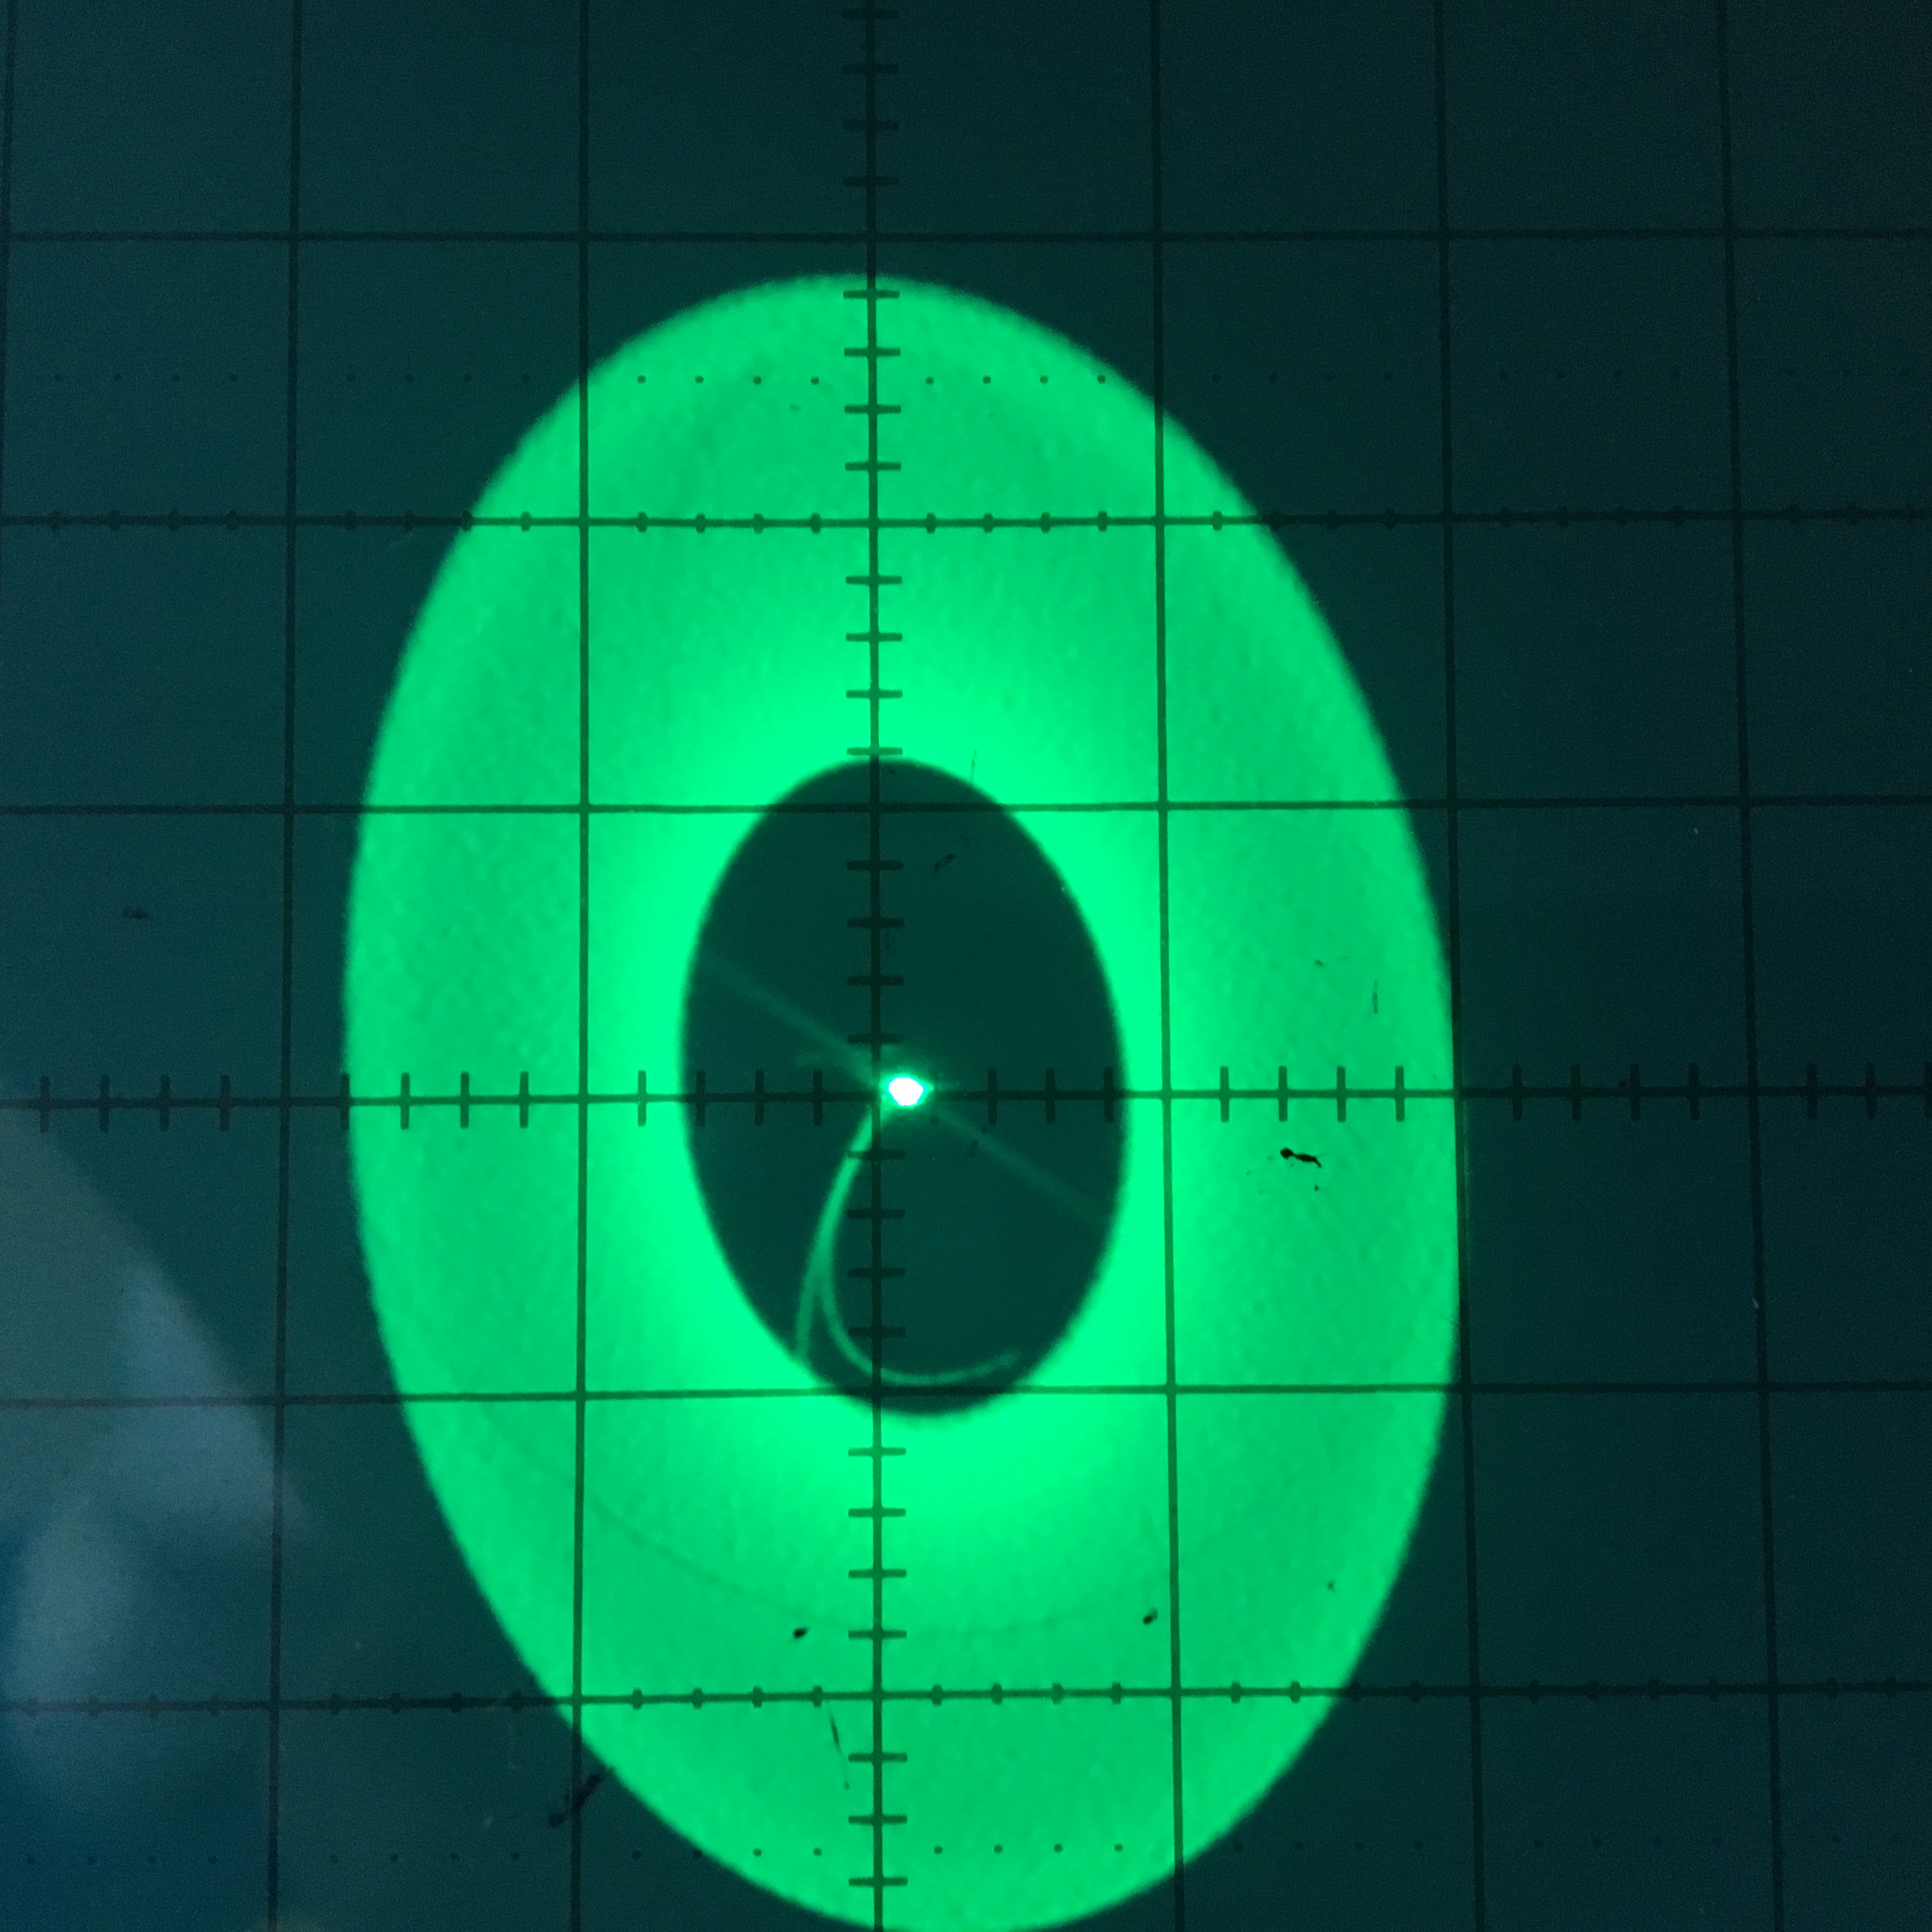
\includegraphics[width=\linewidth]{photo/task3b(midm).jpg}
	\end{minipage}
	\begin{minipage}{0.32\linewidth}
	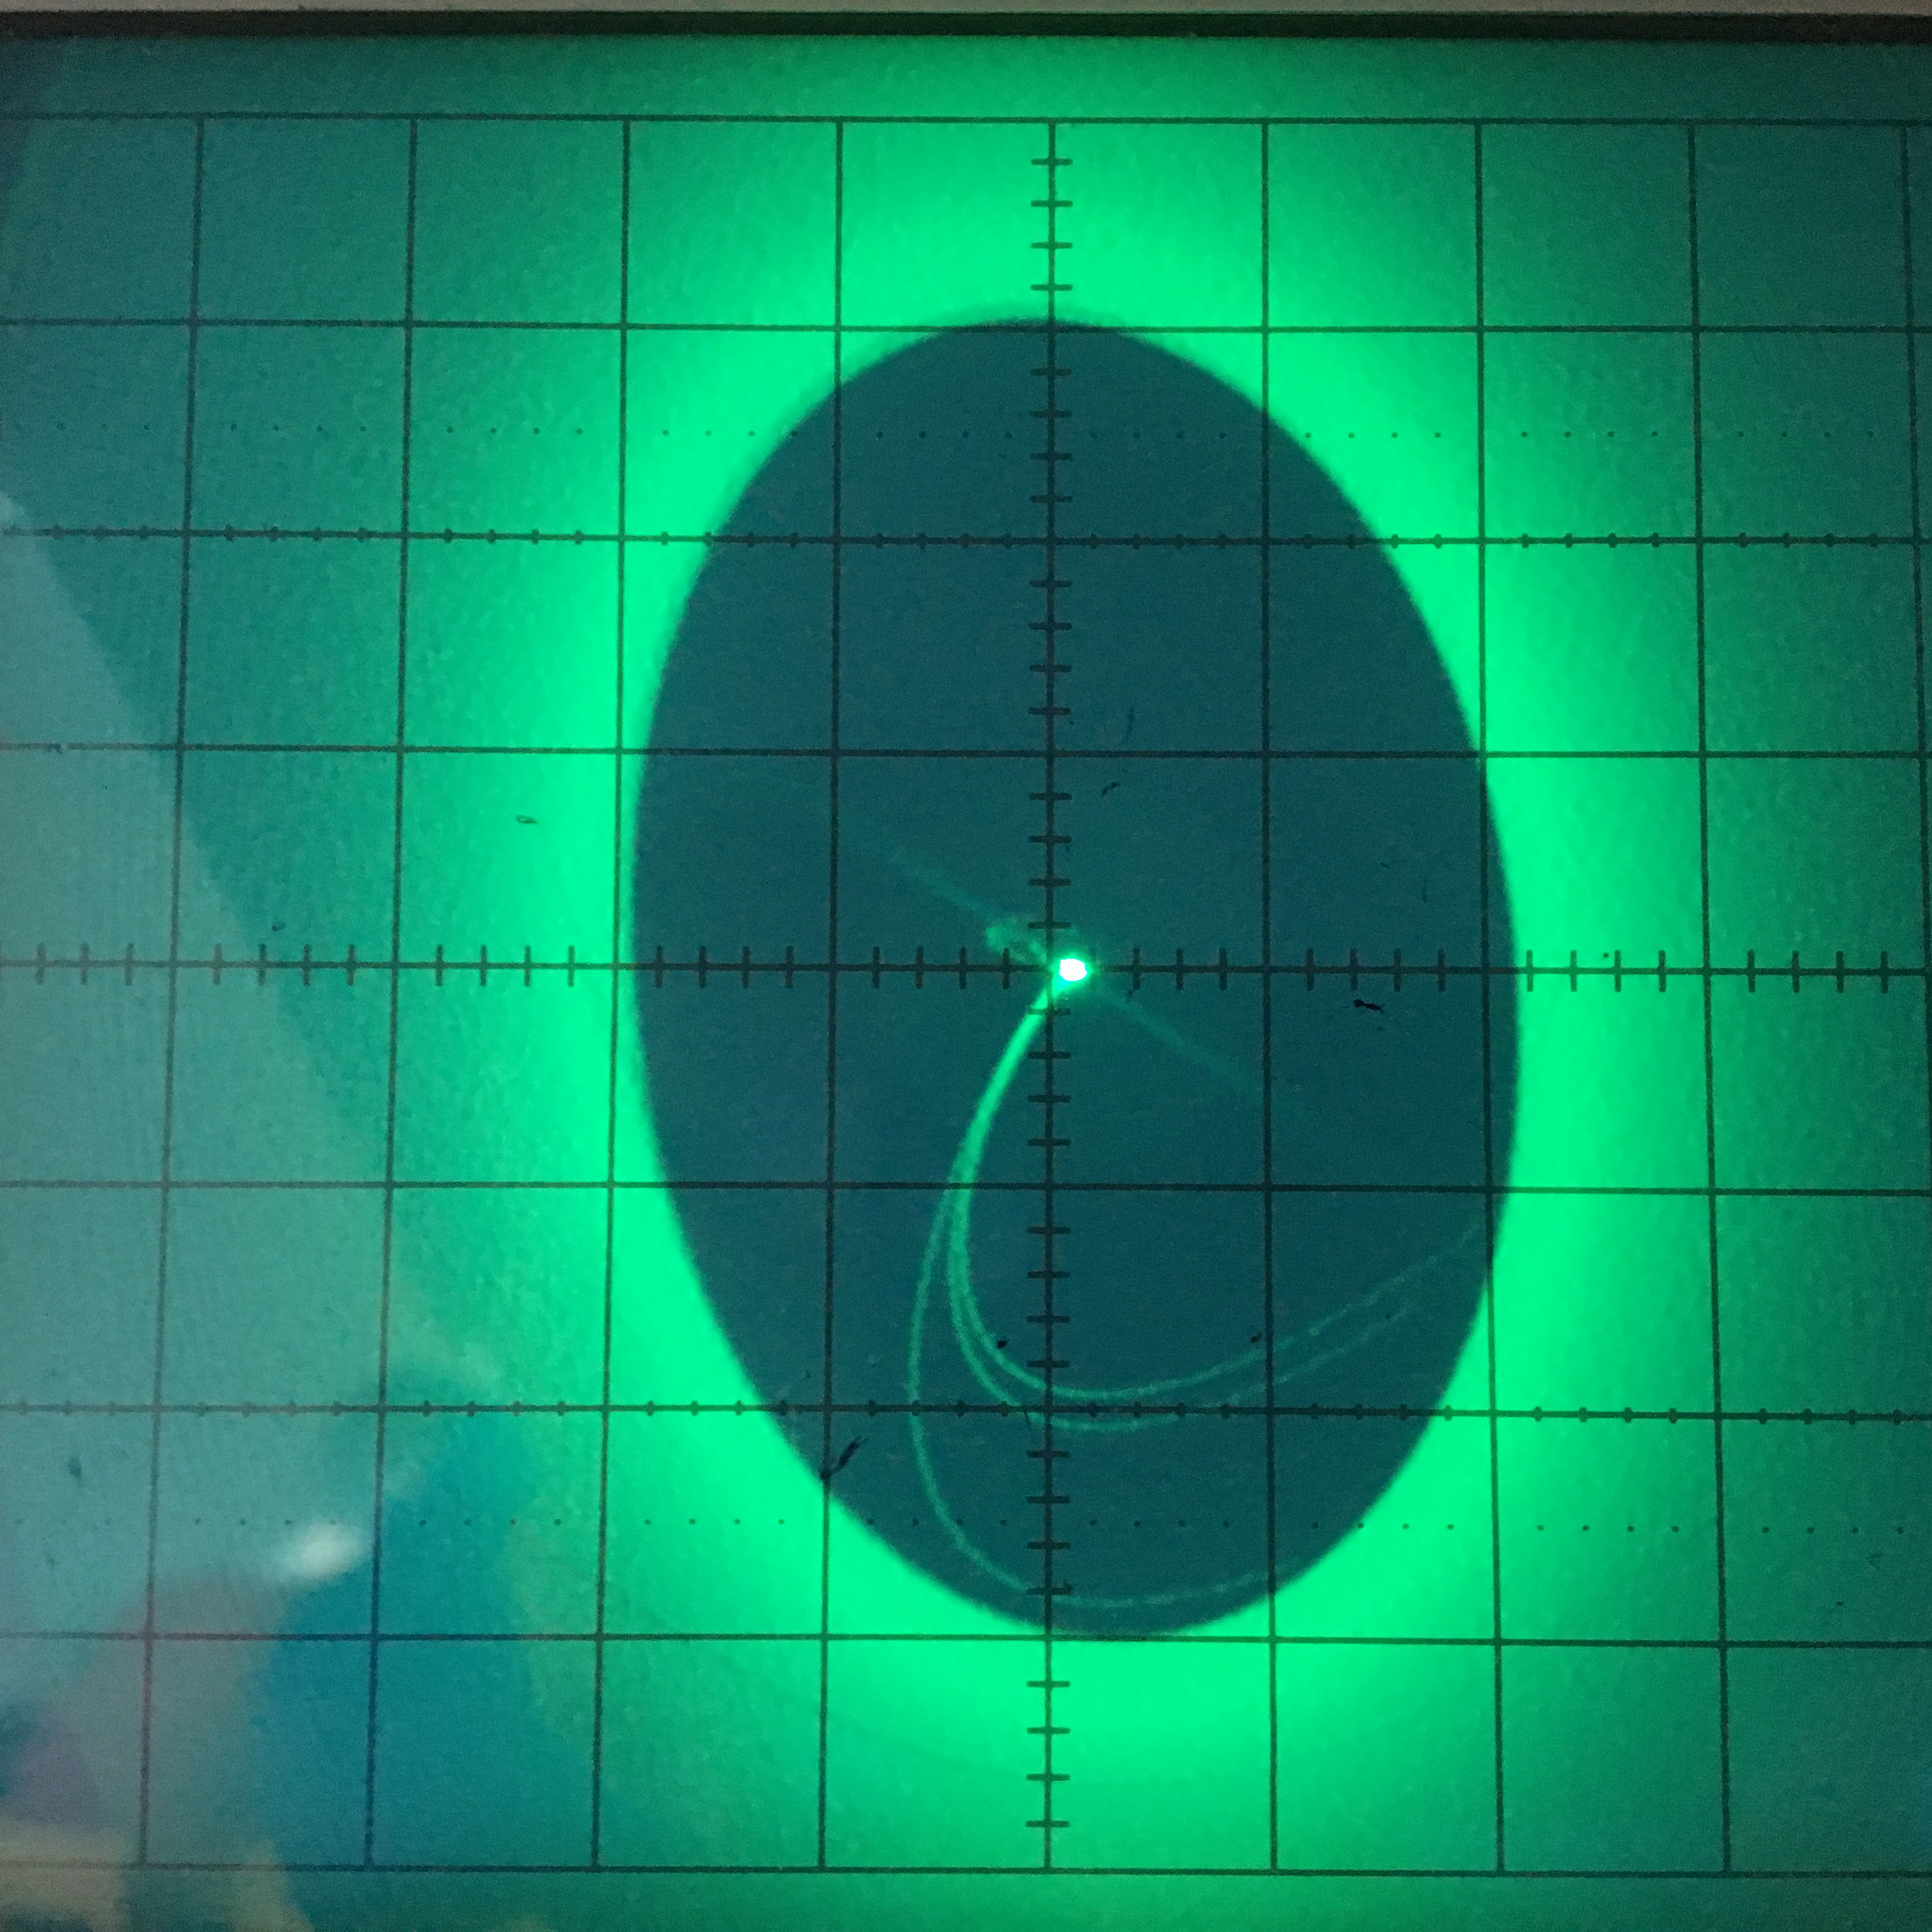
\includegraphics[width=\linewidth]{photo/task3b(midL).jpg}
	\end{minipage}
	\caption{Фазовые траектории при $M'<M<M''$}
	\label{fig14}
\end{figure}
\begin{figure}[h!]
	\centering
	\begin{minipage}{0.32\linewidth}
	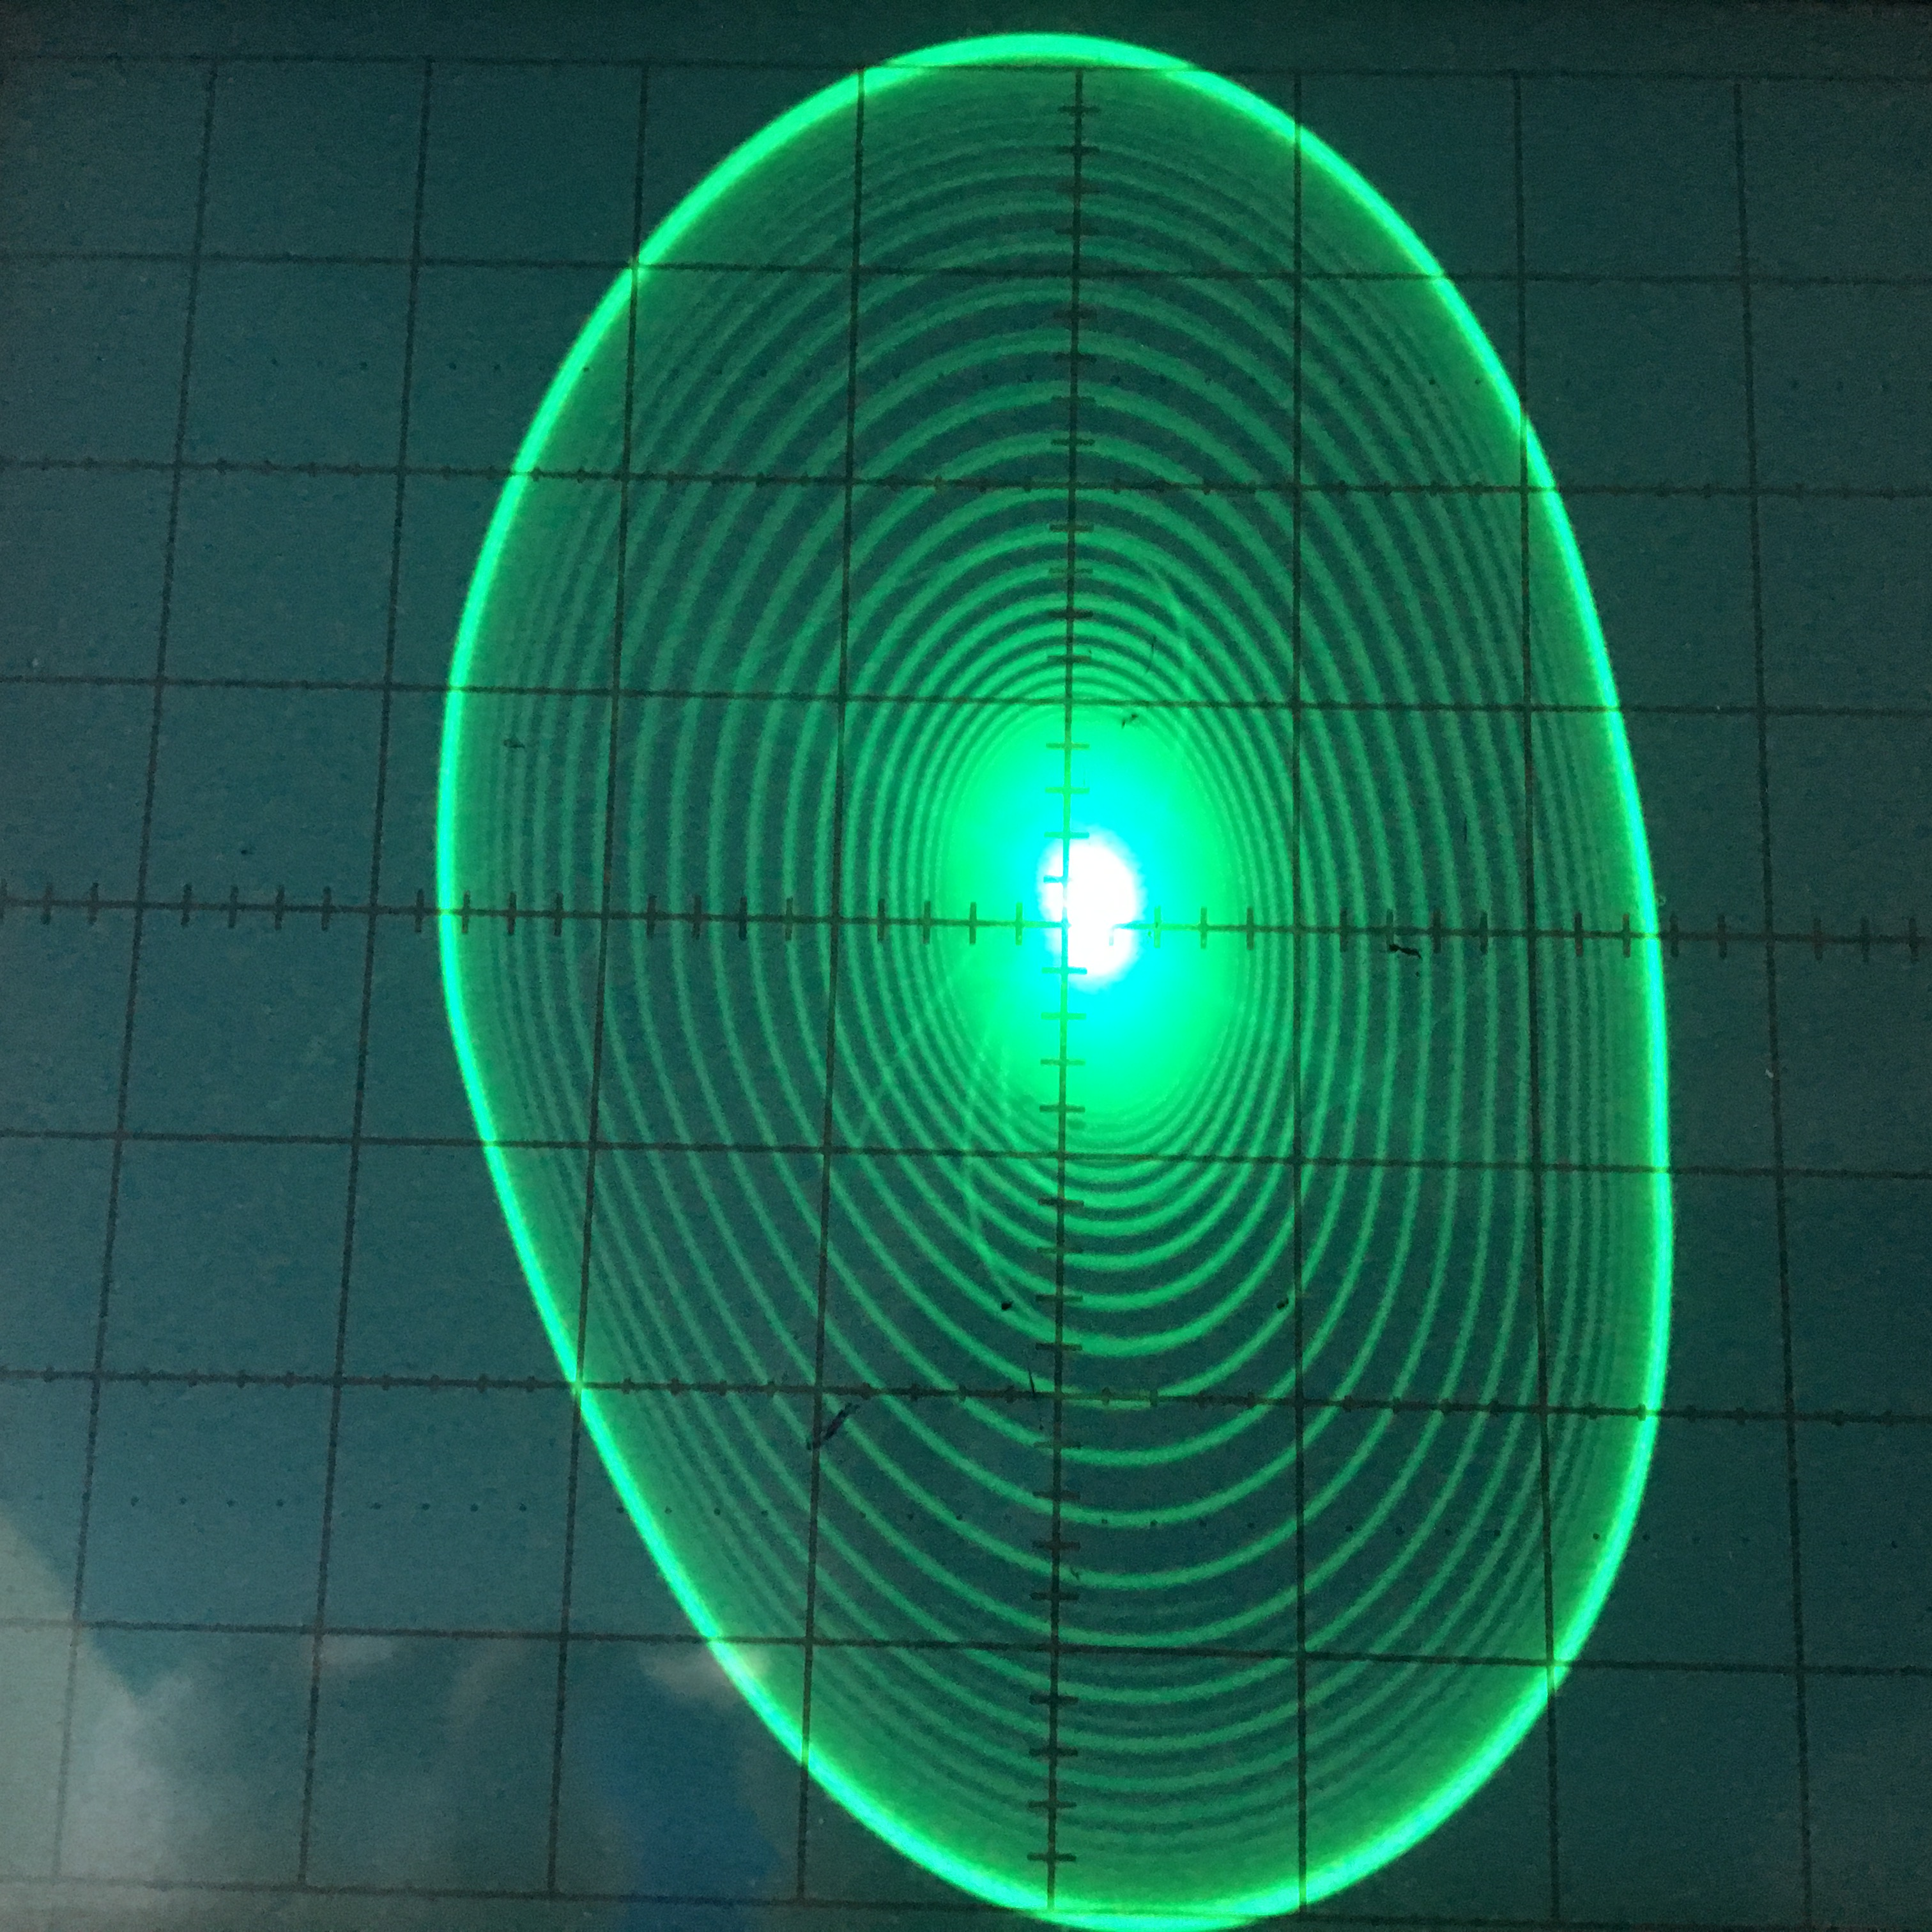
\includegraphics[width=\linewidth]{photo/task3b(rightm).jpg}
	\end{minipage}
	\begin{minipage}{0.32\linewidth}
	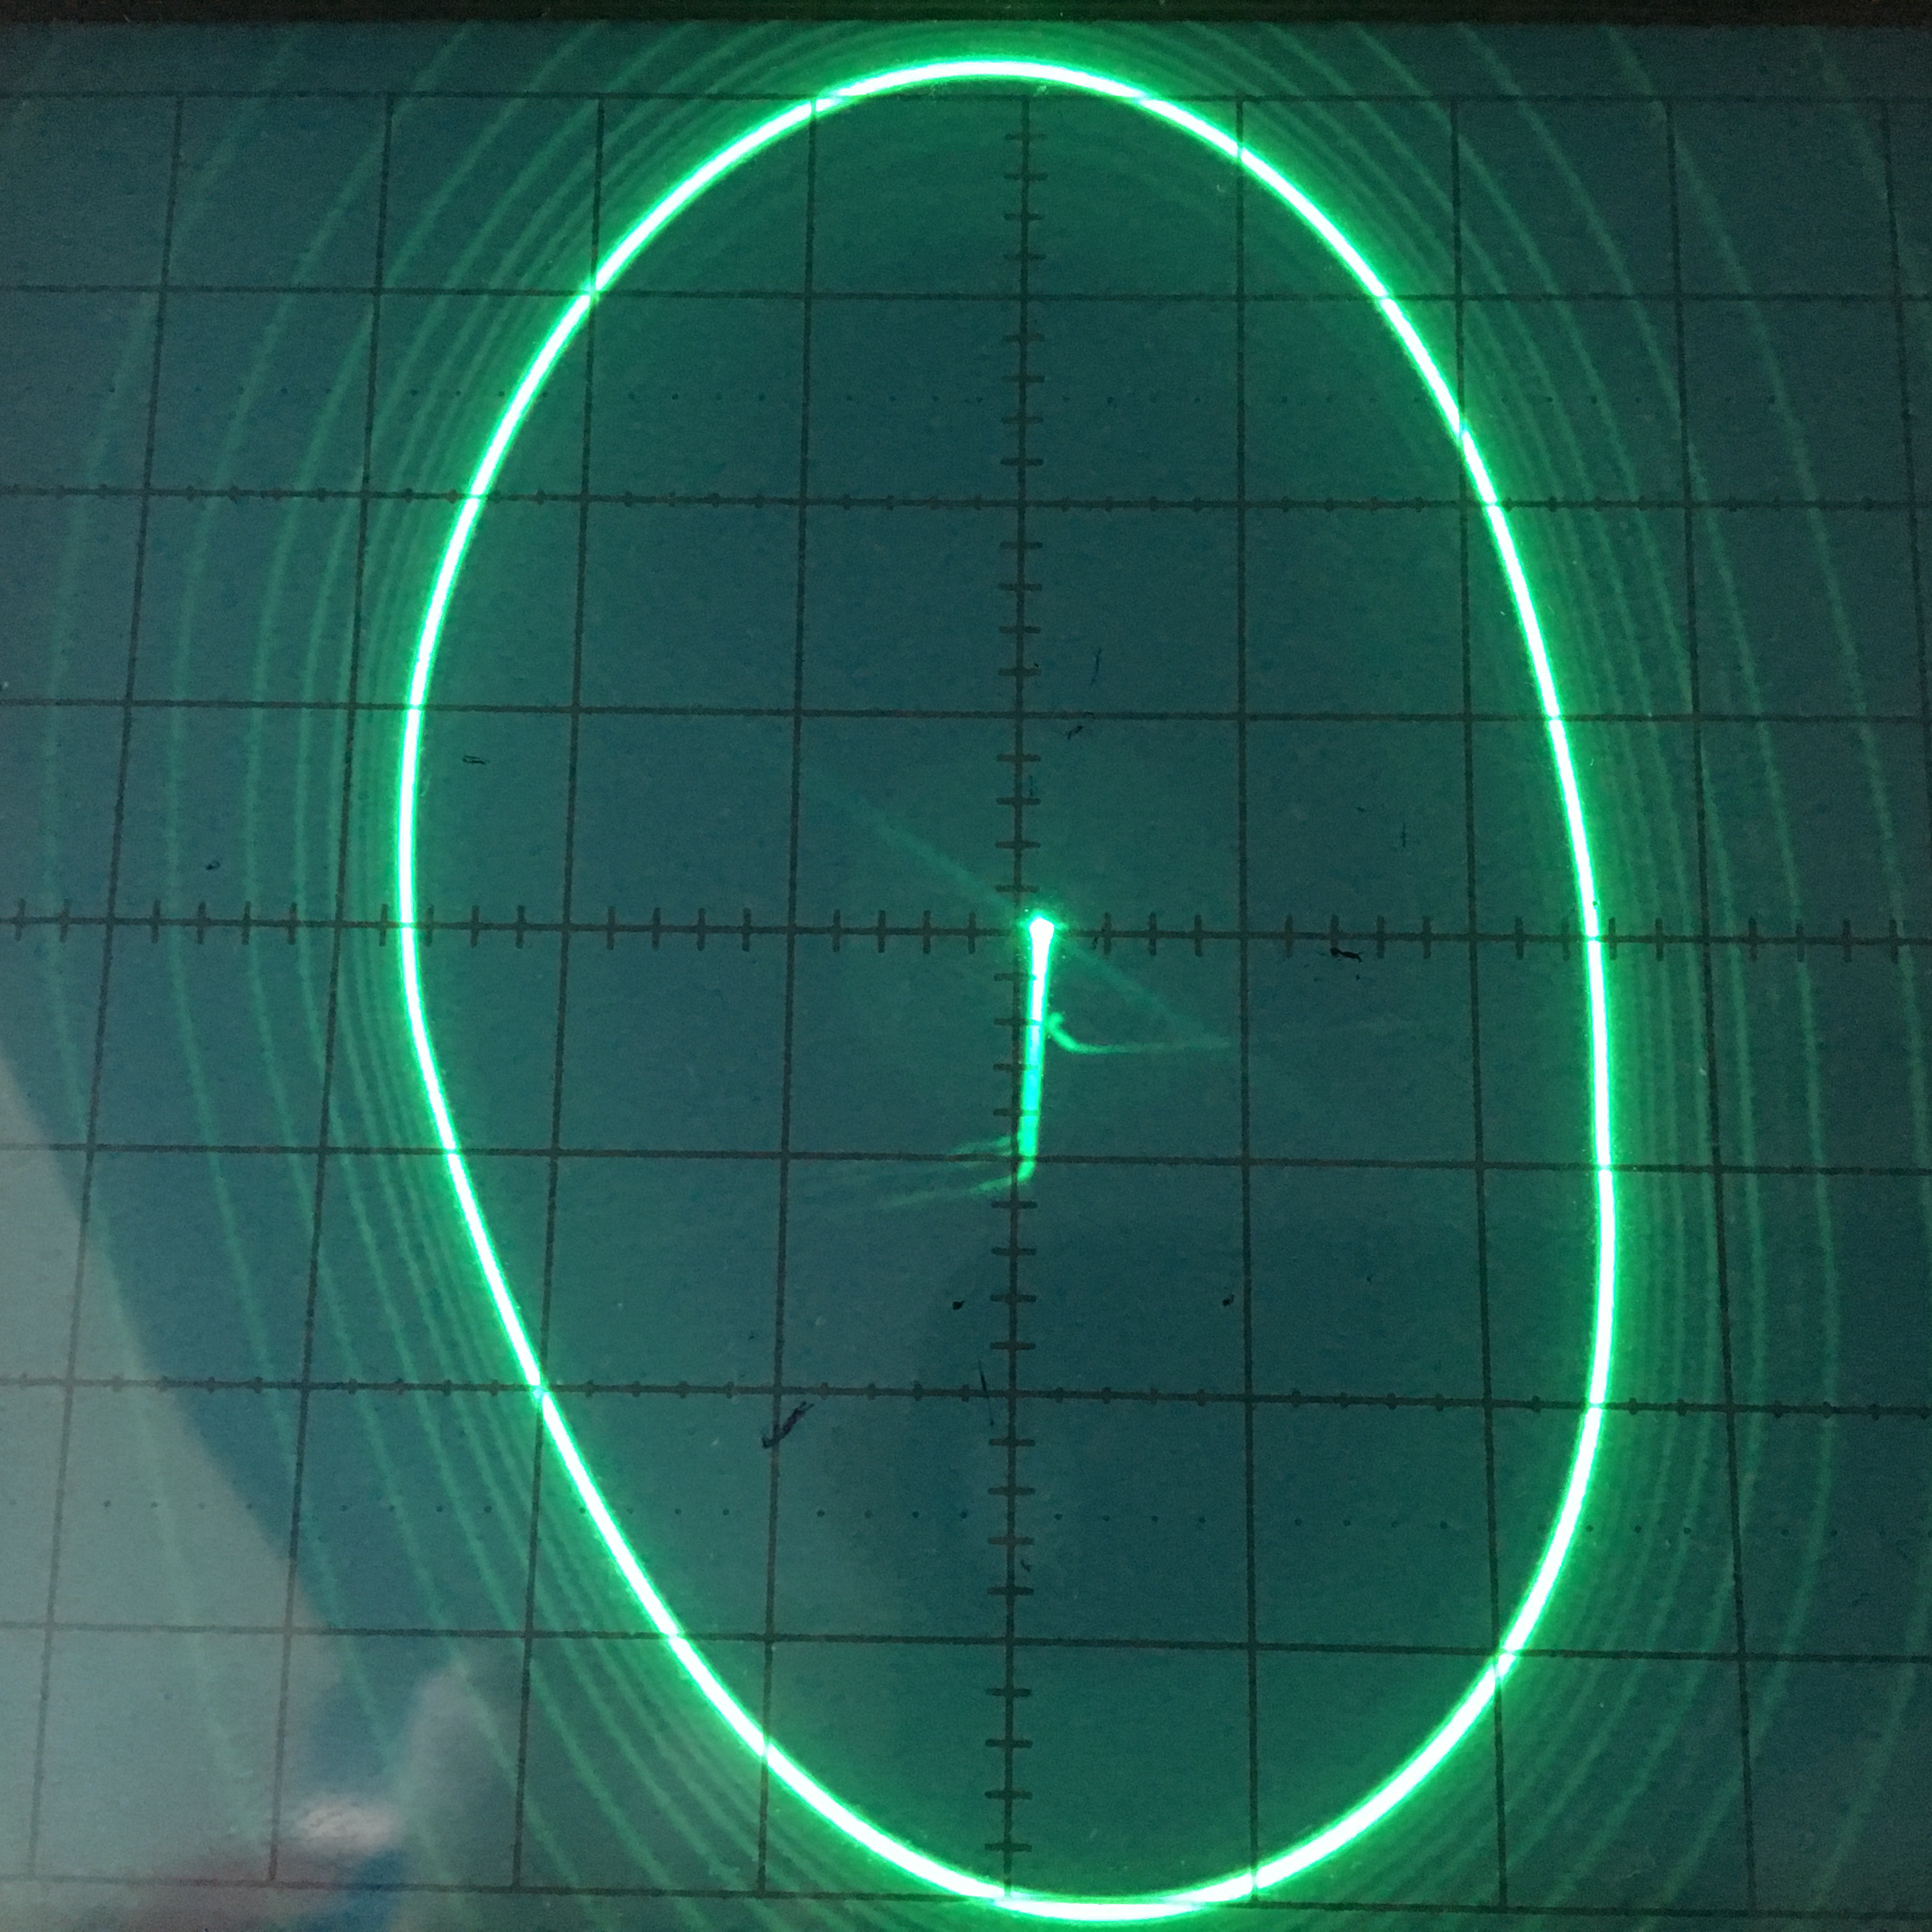
\includegraphics[width=\linewidth]{photo/task3b(rightL).jpg}
	\end{minipage}
	\begin{minipage}{0.32\linewidth}
	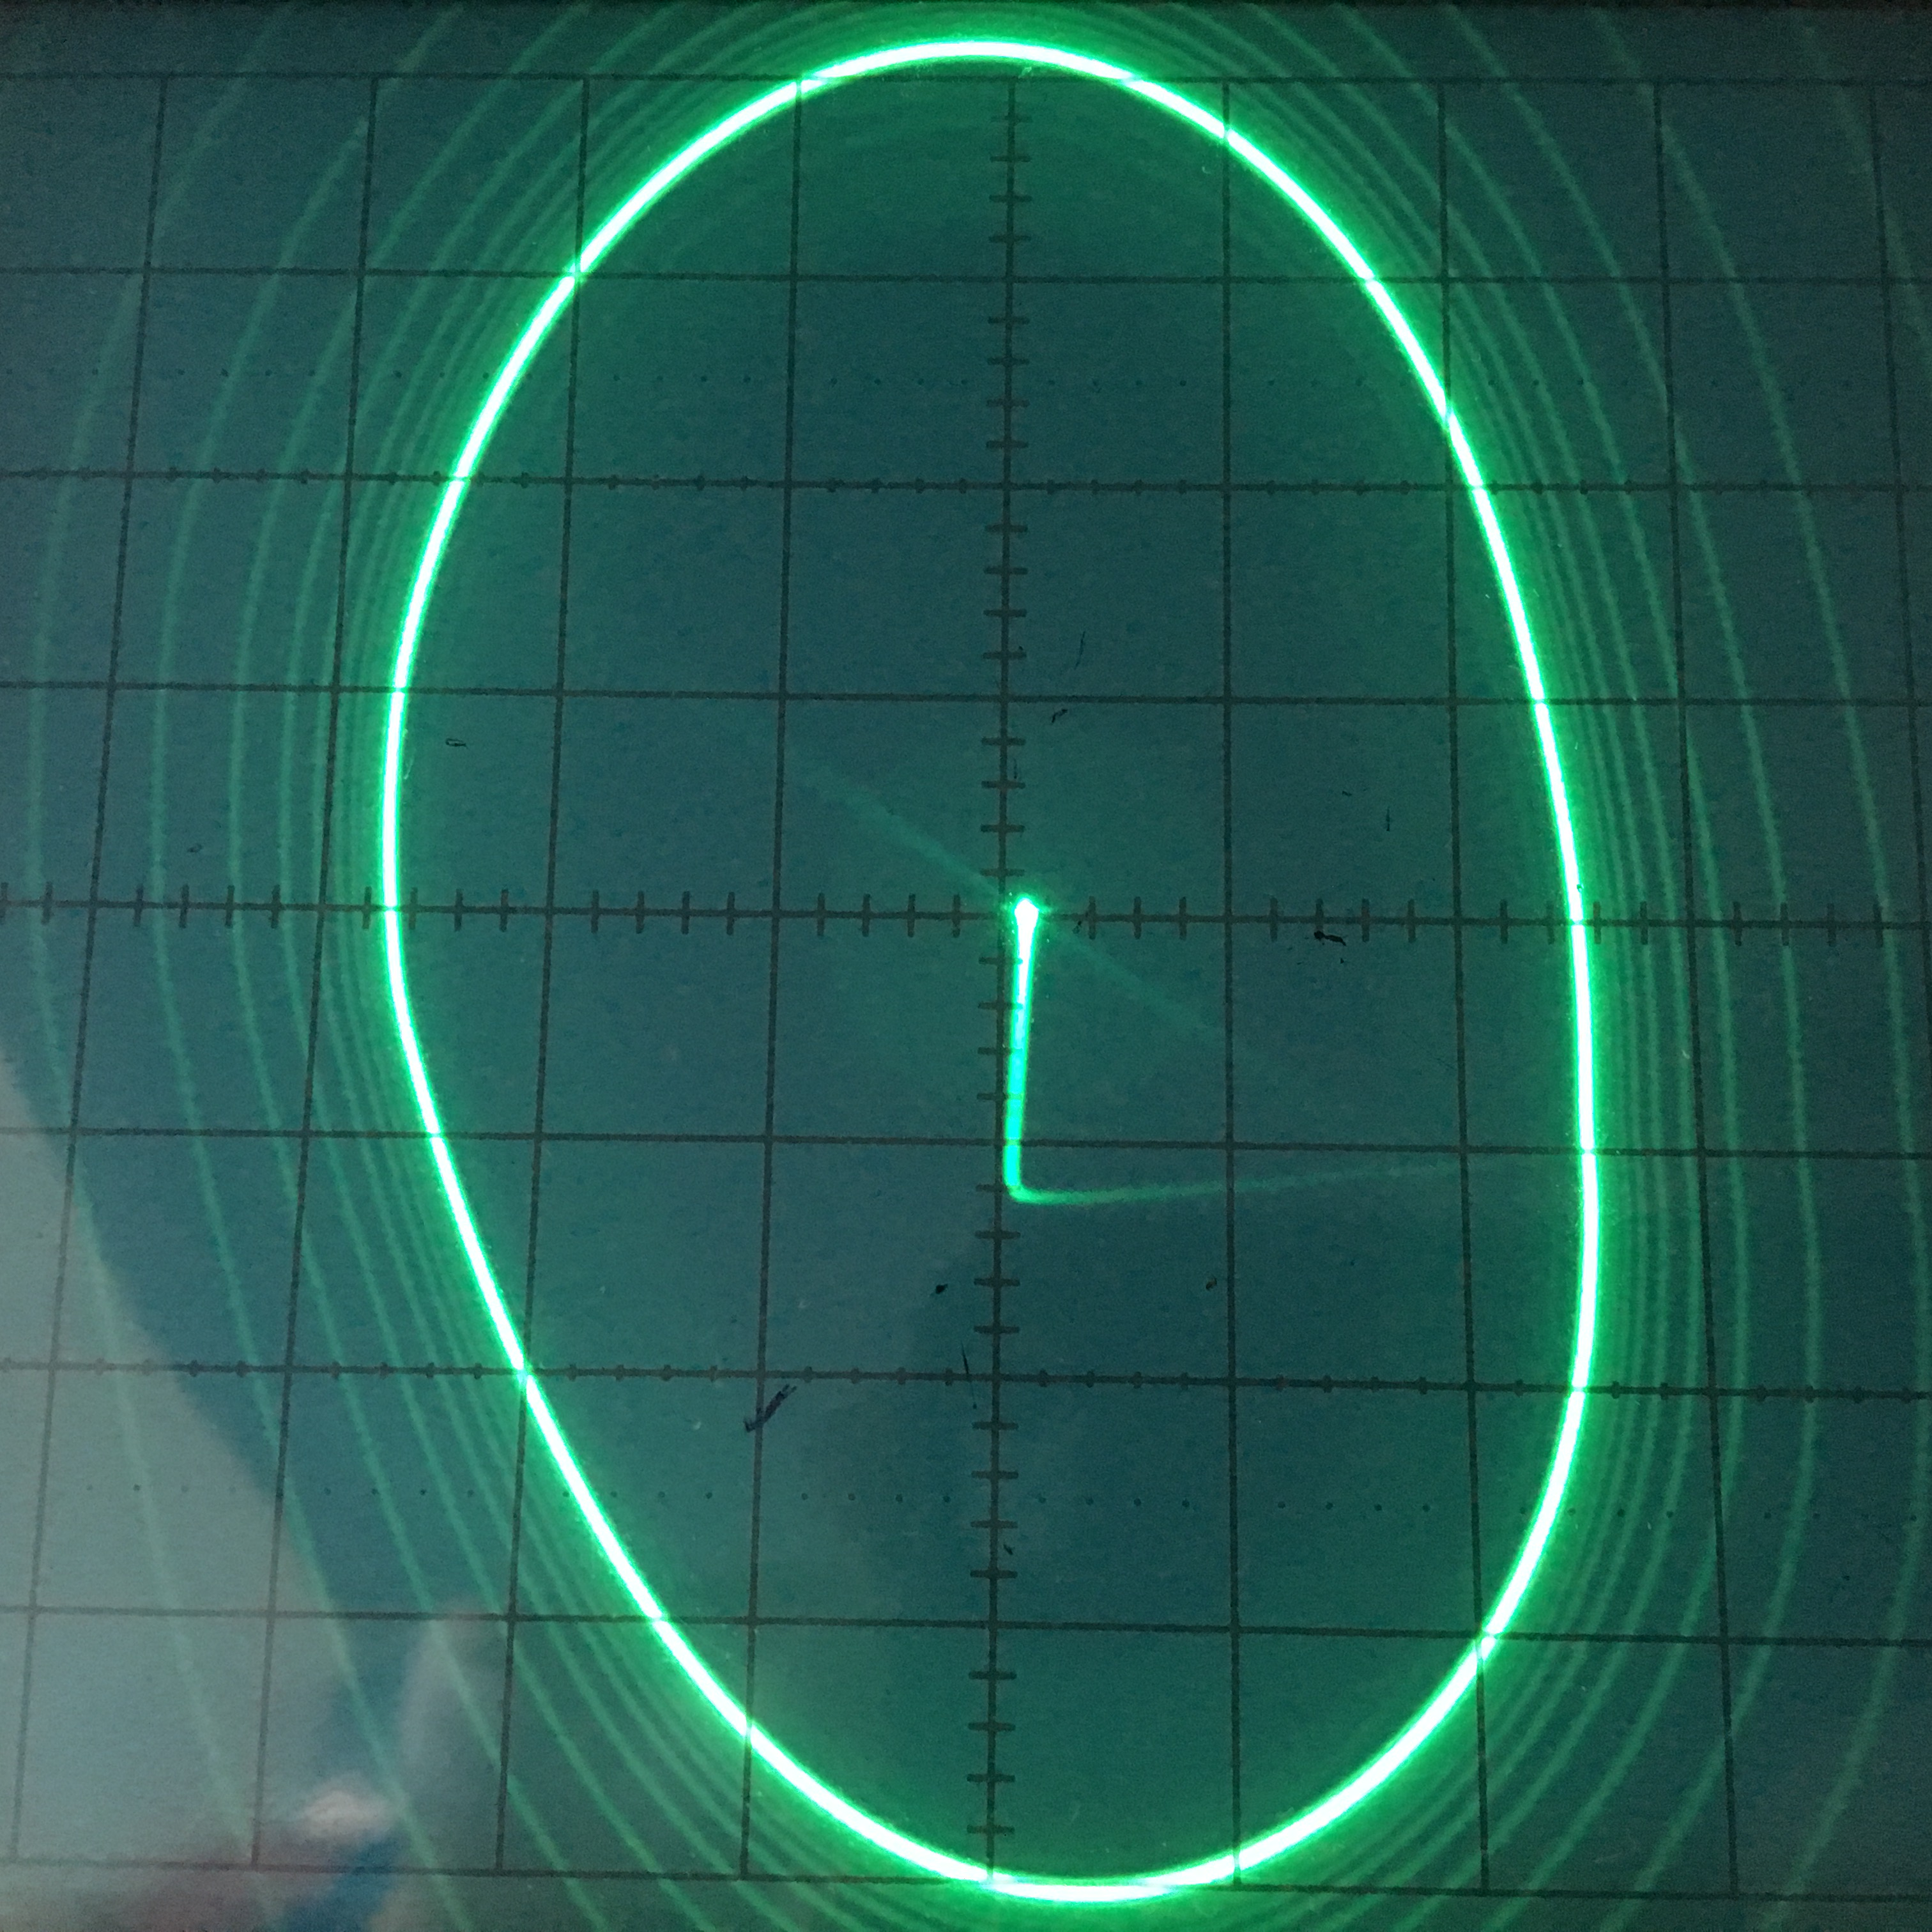
\includegraphics[width=\linewidth]{photo/task3b(rightL2).jpg}
	\end{minipage}
	\caption{Фазовые траектории при $M>M''$}
	\label{fig15}
\end{figure}
Зарисовали фазовые траектории при различных начальных условиях для трех различных значений $М$.
% \afterpage{\clearpage}
\subsection{Вывод}
Изучили различные режимы возбуждения лампового генератора и установили зависимость амплитуды автоколебаний от параметров системы. Построили бифрукационные диаграммы для различных режимов генератора, которые качественно согласуются с теорией, а также рассмотрели фазовые портреты для различных состояний равновесия.
\end{document}

